
\documentclass[10pt]{article} % For LaTeX2e
% \usepackage{tmlr}
% If accepted, instead use the following line for the camera-ready submission:
%\usepackage[accepted]{tmlr}
% To de-anonymize and remove mentions to TMLR (for example for posting to preprint servers), instead use the following:
\usepackage[preprint]{tmlr}

% Optional math commands from https://github.com/goodfeli/dlbook_notation.
%%%%% NEW MATH DEFINITIONS %%%%%

\usepackage{amsmath,amsfonts,bm}

% Mark sections of captions for referring to divisions of figures
\newcommand{\figleft}{{\em (Left)}}
\newcommand{\figcenter}{{\em (Center)}}
\newcommand{\figright}{{\em (Right)}}
\newcommand{\figtop}{{\em (Top)}}
\newcommand{\figbottom}{{\em (Bottom)}}
\newcommand{\captiona}{{\em (a)}}
\newcommand{\captionb}{{\em (b)}}
\newcommand{\captionc}{{\em (c)}}
\newcommand{\captiond}{{\em (d)}}

% Highlight a newly defined term
\newcommand{\newterm}[1]{{\bf #1}}


% Figure reference, lower-case.
\def\figref#1{figure~\ref{#1}}
% Figure reference, capital. For start of sentence
\def\Figref#1{Figure~\ref{#1}}
\def\twofigref#1#2{figures \ref{#1} and \ref{#2}}
\def\quadfigref#1#2#3#4{figures \ref{#1}, \ref{#2}, \ref{#3} and \ref{#4}}
% Section reference, lower-case.
\def\secref#1{section~\ref{#1}}
% Section reference, capital.
\def\Secref#1{Section~\ref{#1}}
% Reference to two sections.
\def\twosecrefs#1#2{sections \ref{#1} and \ref{#2}}
% Reference to three sections.
\def\secrefs#1#2#3{sections \ref{#1}, \ref{#2} and \ref{#3}}
% Reference to an equation, lower-case.
\def\eqref#1{equation~\ref{#1}}
% Reference to an equation, upper case
\def\Eqref#1{Equation~\ref{#1}}
% A raw reference to an equation---avoid using if possible
\def\plaineqref#1{\ref{#1}}
% Reference to a chapter, lower-case.
\def\chapref#1{chapter~\ref{#1}}
% Reference to an equation, upper case.
\def\Chapref#1{Chapter~\ref{#1}}
% Reference to a range of chapters
\def\rangechapref#1#2{chapters\ref{#1}--\ref{#2}}
% Reference to an algorithm, lower-case.
\def\algref#1{algorithm~\ref{#1}}
% Reference to an algorithm, upper case.
\def\Algref#1{Algorithm~\ref{#1}}
\def\twoalgref#1#2{algorithms \ref{#1} and \ref{#2}}
\def\Twoalgref#1#2{Algorithms \ref{#1} and \ref{#2}}
% Reference to a part, lower case
\def\partref#1{part~\ref{#1}}
% Reference to a part, upper case
\def\Partref#1{Part~\ref{#1}}
\def\twopartref#1#2{parts \ref{#1} and \ref{#2}}

\def\ceil#1{\lceil #1 \rceil}
\def\floor#1{\lfloor #1 \rfloor}
\def\1{\bm{1}}
\newcommand{\train}{\mathcal{D}}
\newcommand{\valid}{\mathcal{D_{\mathrm{valid}}}}
\newcommand{\test}{\mathcal{D_{\mathrm{test}}}}

\def\eps{{\epsilon}}


% Random variables
\def\reta{{\textnormal{$\eta$}}}
\def\ra{{\textnormal{a}}}
\def\rb{{\textnormal{b}}}
\def\rc{{\textnormal{c}}}
\def\rd{{\textnormal{d}}}
\def\re{{\textnormal{e}}}
\def\rf{{\textnormal{f}}}
\def\rg{{\textnormal{g}}}
\def\rh{{\textnormal{h}}}
\def\ri{{\textnormal{i}}}
\def\rj{{\textnormal{j}}}
\def\rk{{\textnormal{k}}}
\def\rl{{\textnormal{l}}}
% rm is already a command, just don't name any random variables m
\def\rn{{\textnormal{n}}}
\def\ro{{\textnormal{o}}}
\def\rp{{\textnormal{p}}}
\def\rq{{\textnormal{q}}}
\def\rr{{\textnormal{r}}}
\def\rs{{\textnormal{s}}}
\def\rt{{\textnormal{t}}}
\def\ru{{\textnormal{u}}}
\def\rv{{\textnormal{v}}}
\def\rw{{\textnormal{w}}}
\def\rx{{\textnormal{x}}}
\def\ry{{\textnormal{y}}}
\def\rz{{\textnormal{z}}}

% Random vectors
\def\rvepsilon{{\mathbf{\epsilon}}}
\def\rvtheta{{\mathbf{\theta}}}
\def\rva{{\mathbf{a}}}
\def\rvb{{\mathbf{b}}}
\def\rvc{{\mathbf{c}}}
\def\rvd{{\mathbf{d}}}
\def\rve{{\mathbf{e}}}
\def\rvf{{\mathbf{f}}}
\def\rvg{{\mathbf{g}}}
\def\rvh{{\mathbf{h}}}
\def\rvu{{\mathbf{i}}}
\def\rvj{{\mathbf{j}}}
\def\rvk{{\mathbf{k}}}
\def\rvl{{\mathbf{l}}}
\def\rvm{{\mathbf{m}}}
\def\rvn{{\mathbf{n}}}
\def\rvo{{\mathbf{o}}}
\def\rvp{{\mathbf{p}}}
\def\rvq{{\mathbf{q}}}
\def\rvr{{\mathbf{r}}}
\def\rvs{{\mathbf{s}}}
\def\rvt{{\mathbf{t}}}
\def\rvu{{\mathbf{u}}}
\def\rvv{{\mathbf{v}}}
\def\rvw{{\mathbf{w}}}
\def\rvx{{\mathbf{x}}}
\def\rvy{{\mathbf{y}}}
\def\rvz{{\mathbf{z}}}

% Elements of random vectors
\def\erva{{\textnormal{a}}}
\def\ervb{{\textnormal{b}}}
\def\ervc{{\textnormal{c}}}
\def\ervd{{\textnormal{d}}}
\def\erve{{\textnormal{e}}}
\def\ervf{{\textnormal{f}}}
\def\ervg{{\textnormal{g}}}
\def\ervh{{\textnormal{h}}}
\def\ervi{{\textnormal{i}}}
\def\ervj{{\textnormal{j}}}
\def\ervk{{\textnormal{k}}}
\def\ervl{{\textnormal{l}}}
\def\ervm{{\textnormal{m}}}
\def\ervn{{\textnormal{n}}}
\def\ervo{{\textnormal{o}}}
\def\ervp{{\textnormal{p}}}
\def\ervq{{\textnormal{q}}}
\def\ervr{{\textnormal{r}}}
\def\ervs{{\textnormal{s}}}
\def\ervt{{\textnormal{t}}}
\def\ervu{{\textnormal{u}}}
\def\ervv{{\textnormal{v}}}
\def\ervw{{\textnormal{w}}}
\def\ervx{{\textnormal{x}}}
\def\ervy{{\textnormal{y}}}
\def\ervz{{\textnormal{z}}}

% Random matrices
\def\rmA{{\mathbf{A}}}
\def\rmB{{\mathbf{B}}}
\def\rmC{{\mathbf{C}}}
\def\rmD{{\mathbf{D}}}
\def\rmE{{\mathbf{E}}}
\def\rmF{{\mathbf{F}}}
\def\rmG{{\mathbf{G}}}
\def\rmH{{\mathbf{H}}}
\def\rmI{{\mathbf{I}}}
\def\rmJ{{\mathbf{J}}}
\def\rmK{{\mathbf{K}}}
\def\rmL{{\mathbf{L}}}
\def\rmM{{\mathbf{M}}}
\def\rmN{{\mathbf{N}}}
\def\rmO{{\mathbf{O}}}
\def\rmP{{\mathbf{P}}}
\def\rmQ{{\mathbf{Q}}}
\def\rmR{{\mathbf{R}}}
\def\rmS{{\mathbf{S}}}
\def\rmT{{\mathbf{T}}}
\def\rmU{{\mathbf{U}}}
\def\rmV{{\mathbf{V}}}
\def\rmW{{\mathbf{W}}}
\def\rmX{{\mathbf{X}}}
\def\rmY{{\mathbf{Y}}}
\def\rmZ{{\mathbf{Z}}}

% Elements of random matrices
\def\ermA{{\textnormal{A}}}
\def\ermB{{\textnormal{B}}}
\def\ermC{{\textnormal{C}}}
\def\ermD{{\textnormal{D}}}
\def\ermE{{\textnormal{E}}}
\def\ermF{{\textnormal{F}}}
\def\ermG{{\textnormal{G}}}
\def\ermH{{\textnormal{H}}}
\def\ermI{{\textnormal{I}}}
\def\ermJ{{\textnormal{J}}}
\def\ermK{{\textnormal{K}}}
\def\ermL{{\textnormal{L}}}
\def\ermM{{\textnormal{M}}}
\def\ermN{{\textnormal{N}}}
\def\ermO{{\textnormal{O}}}
\def\ermP{{\textnormal{P}}}
\def\ermQ{{\textnormal{Q}}}
\def\ermR{{\textnormal{R}}}
\def\ermS{{\textnormal{S}}}
\def\ermT{{\textnormal{T}}}
\def\ermU{{\textnormal{U}}}
\def\ermV{{\textnormal{V}}}
\def\ermW{{\textnormal{W}}}
\def\ermX{{\textnormal{X}}}
\def\ermY{{\textnormal{Y}}}
\def\ermZ{{\textnormal{Z}}}

% Vectors
\def\vzero{{\bm{0}}}
\def\vone{{\bm{1}}}
\def\vmu{{\bm{\mu}}}
\def\vtheta{{\bm{\theta}}}
\def\vpsi{{\bm{\psi}}}
\def\vsigma{{\bm{\sigma}}}
\def\vlambda{{\bm{\lambda}}}
\def\vgamma{{\bm{\gamma}}}
\def\vomega{{\bm{\omega}}}
\def\va{{\bm{a}}}
\def\vb{{\bm{b}}}
\def\vc{{\bm{c}}}
\def\vd{{\bm{d}}}
\def\ve{{\bm{e}}}
\def\vf{{\bm{f}}}
\def\vg{{\bm{g}}}
\def\vh{{\bm{h}}}
\def\vi{{\bm{i}}}
\def\vj{{\bm{j}}}
\def\vk{{\bm{k}}}
\def\vl{{\bm{l}}}
\def\vm{{\bm{m}}}
\def\vn{{\bm{n}}}
\def\vo{{\bm{o}}}
\def\vp{{\bm{p}}}
\def\vq{{\bm{q}}}
\def\vr{{\bm{r}}}
\def\vs{{\bm{s}}}
\def\vt{{\bm{t}}}
\def\vu{{\bm{u}}}
\def\vv{{\bm{v}}}
\def\vw{{\bm{w}}}
\def\vx{{\bm{x}}}
\def\vy{{\bm{y}}}
\def\vz{{\bm{z}}}

% Elements of vectors
\def\evalpha{{\alpha}}
\def\evbeta{{\beta}}
\def\evepsilon{{\epsilon}}
\def\evlambda{{\lambda}}
\def\evomega{{\omega}}
\def\evmu{{\mu}}
\def\evpsi{{\psi}}
\def\evsigma{{\sigma}}
\def\evtheta{{\theta}}
\def\evgamma{{\gamma}}
\def\eva{{a}}
\def\evb{{b}}
\def\evc{{c}}
\def\evd{{d}}
\def\eve{{e}}
\def\evf{{f}}
\def\evg{{g}}
\def\evh{{h}}
\def\evi{{i}}
\def\evj{{j}}
\def\evk{{k}}
\def\evl{{l}}
\def\evm{{m}}
\def\evn{{n}}
\def\evo{{o}}
\def\evp{{p}}
\def\evq{{q}}
\def\evr{{r}}
\def\evs{{s}}
\def\evt{{t}}
\def\evu{{u}}
\def\evv{{v}}
\def\evw{{w}}
\def\evx{{x}}
\def\evy{{y}}
\def\evz{{z}}

% Matrix
\def\mA{{\bm{A}}}
\def\mB{{\bm{B}}}
\def\mC{{\bm{C}}}
\def\mD{{\bm{D}}}
\def\mE{{\bm{E}}}
\def\mF{{\bm{F}}}
\def\mG{{\bm{G}}}
\def\mH{{\bm{H}}}
\def\mI{{\bm{I}}}
\def\mJ{{\bm{J}}}
\def\mK{{\bm{K}}}
\def\mL{{\bm{L}}}
\def\mM{{\bm{M}}}
\def\mN{{\bm{N}}}
\def\mO{{\bm{O}}}
\def\mP{{\bm{P}}}
\def\mQ{{\bm{Q}}}
\def\mR{{\bm{R}}}
\def\mS{{\bm{S}}}
\def\mT{{\bm{T}}}
\def\mU{{\bm{U}}}
\def\mV{{\bm{V}}}
\def\mW{{\bm{W}}}
\def\mX{{\bm{X}}}
\def\mY{{\bm{Y}}}
\def\mZ{{\bm{Z}}}
\def\mBeta{{\bm{\beta}}}
\def\mPhi{{\bm{\Phi}}}
\def\mPsi{{\bm{\Psi}}}
\def\mTheta{{\bm{\Theta}}}
\def\mLambda{{\bm{\Lambda}}}
\def\mSigma{{\bm{\Sigma}}}

% Tensor
\DeclareMathAlphabet{\mathsfit}{\encodingdefault}{\sfdefault}{m}{sl}
\SetMathAlphabet{\mathsfit}{bold}{\encodingdefault}{\sfdefault}{bx}{n}
\newcommand{\tens}[1]{\bm{\mathsfit{#1}}}
\def\tA{{\tens{A}}}
\def\tB{{\tens{B}}}
\def\tC{{\tens{C}}}
\def\tD{{\tens{D}}}
\def\tE{{\tens{E}}}
\def\tF{{\tens{F}}}
\def\tG{{\tens{G}}}
\def\tH{{\tens{H}}}
\def\tI{{\tens{I}}}
\def\tJ{{\tens{J}}}
\def\tK{{\tens{K}}}
\def\tL{{\tens{L}}}
\def\tM{{\tens{M}}}
\def\tN{{\tens{N}}}
\def\tO{{\tens{O}}}
\def\tP{{\tens{P}}}
\def\tQ{{\tens{Q}}}
\def\tR{{\tens{R}}}
\def\tS{{\tens{S}}}
\def\tT{{\tens{T}}}
\def\tU{{\tens{U}}}
\def\tV{{\tens{V}}}
\def\tW{{\tens{W}}}
\def\tX{{\tens{X}}}
\def\tY{{\tens{Y}}}
\def\tZ{{\tens{Z}}}


% Graph
\def\gA{{\mathcal{A}}}
\def\gB{{\mathcal{B}}}
\def\gC{{\mathcal{C}}}
\def\gD{{\mathcal{D}}}
\def\gE{{\mathcal{E}}}
\def\gF{{\mathcal{F}}}
\def\gG{{\mathcal{G}}}
\def\gH{{\mathcal{H}}}
\def\gI{{\mathcal{I}}}
\def\gJ{{\mathcal{J}}}
\def\gK{{\mathcal{K}}}
\def\gL{{\mathcal{L}}}
\def\gM{{\mathcal{M}}}
\def\gN{{\mathcal{N}}}
\def\gO{{\mathcal{O}}}
\def\gP{{\mathcal{P}}}
\def\gQ{{\mathcal{Q}}}
\def\gR{{\mathcal{R}}}
\def\gS{{\mathcal{S}}}
\def\gT{{\mathcal{T}}}
\def\gU{{\mathcal{U}}}
\def\gV{{\mathcal{V}}}
\def\gW{{\mathcal{W}}}
\def\gX{{\mathcal{X}}}
\def\gY{{\mathcal{Y}}}
\def\gZ{{\mathcal{Z}}}

% Sets
\def\sA{{\mathbb{A}}}
\def\sB{{\mathbb{B}}}
\def\sC{{\mathbb{C}}}
\def\sD{{\mathbb{D}}}
% Don't use a set called E, because this would be the same as our symbol
% for expectation.
\def\sF{{\mathbb{F}}}
\def\sG{{\mathbb{G}}}
\def\sH{{\mathbb{H}}}
\def\sI{{\mathbb{I}}}
\def\sJ{{\mathbb{J}}}
\def\sK{{\mathbb{K}}}
\def\sL{{\mathbb{L}}}
\def\sM{{\mathbb{M}}}
\def\sN{{\mathbb{N}}}
\def\sO{{\mathbb{O}}}
\def\sP{{\mathbb{P}}}
\def\sQ{{\mathbb{Q}}}
\def\sR{{\mathbb{R}}}
\def\sS{{\mathbb{S}}}
\def\sT{{\mathbb{T}}}
\def\sU{{\mathbb{U}}}
\def\sV{{\mathbb{V}}}
\def\sW{{\mathbb{W}}}
\def\sX{{\mathbb{X}}}
\def\sY{{\mathbb{Y}}}
\def\sZ{{\mathbb{Z}}}

% Entries of a matrix
\def\emLambda{{\Lambda}}
\def\emA{{A}}
\def\emB{{B}}
\def\emC{{C}}
\def\emD{{D}}
\def\emE{{E}}
\def\emF{{F}}
\def\emG{{G}}
\def\emH{{H}}
\def\emI{{I}}
\def\emJ{{J}}
\def\emK{{K}}
\def\emL{{L}}
\def\emM{{M}}
\def\emN{{N}}
\def\emO{{O}}
\def\emP{{P}}
\def\emQ{{Q}}
\def\emR{{R}}
\def\emS{{S}}
\def\emT{{T}}
\def\emU{{U}}
\def\emV{{V}}
\def\emW{{W}}
\def\emX{{X}}
\def\emY{{Y}}
\def\emZ{{Z}}
\def\emSigma{{\Sigma}}
\def\emPhi{{\Phi}}
\def\emPsi{{\Psi}}
\def\emTheta{{\Theta}}




% entries of a tensor
% Same font as tensor, without \bm wrapper
\newcommand{\etens}[1]{\mathsfit{#1}}
\def\etLambda{{\etens{\Lambda}}}
\def\etA{{\etens{A}}}
\def\etB{{\etens{B}}}
\def\etC{{\etens{C}}}
\def\etD{{\etens{D}}}
\def\etE{{\etens{E}}}
\def\etF{{\etens{F}}}
\def\etG{{\etens{G}}}
\def\etH{{\etens{H}}}
\def\etI{{\etens{I}}}
\def\etJ{{\etens{J}}}
\def\etK{{\etens{K}}}
\def\etL{{\etens{L}}}
\def\etM{{\etens{M}}}
\def\etN{{\etens{N}}}
\def\etO{{\etens{O}}}
\def\etP{{\etens{P}}}
\def\etQ{{\etens{Q}}}
\def\etR{{\etens{R}}}
\def\etS{{\etens{S}}}
\def\etT{{\etens{T}}}
\def\etU{{\etens{U}}}
\def\etV{{\etens{V}}}
\def\etW{{\etens{W}}}
\def\etX{{\etens{X}}}
\def\etY{{\etens{Y}}}
\def\etZ{{\etens{Z}}}

% The true underlying data generating distribution
\newcommand{\pdata}{p_{\rm{data}}}
% The empirical distribution defined by the training set
\newcommand{\ptrain}{\hat{p}_{\rm{data}}}
\newcommand{\Ptrain}{\hat{P}_{\rm{data}}}
% The model distribution
\newcommand{\pmodel}{p_{\rm{model}}}
\newcommand{\Pmodel}{P_{\rm{model}}}
\newcommand{\ptildemodel}{\tilde{p}_{\rm{model}}}
% Stochastic autoencoder distributions
\newcommand{\pencode}{p_{\rm{encoder}}}
\newcommand{\pdecode}{p_{\rm{decoder}}}
\newcommand{\precons}{p_{\rm{reconstruct}}}

\newcommand{\laplace}{\mathrm{Laplace}} % Laplace distribution

\newcommand{\E}{\mathbb{E}}
\newcommand{\Ls}{\mathcal{L}}
\newcommand{\R}{\mathbb{R}}
\newcommand{\emp}{\tilde{p}}
\newcommand{\lr}{\alpha}
\newcommand{\reg}{\lambda}
\newcommand{\rect}{\mathrm{rectifier}}
\newcommand{\softmax}{\mathrm{softmax}}
\newcommand{\sigmoid}{\sigma}
\newcommand{\softplus}{\zeta}
\newcommand{\KL}{D_{\mathrm{KL}}}
\newcommand{\Var}{\mathrm{Var}}
\newcommand{\standarderror}{\mathrm{SE}}
\newcommand{\Cov}{\mathrm{Cov}}
% Wolfram Mathworld says $L^2$ is for function spaces and $\ell^2$ is for vectors
% But then they seem to use $L^2$ for vectors throughout the site, and so does
% wikipedia.
\newcommand{\normlzero}{L^0}
\newcommand{\normlone}{L^1}
\newcommand{\normltwo}{L^2}
\newcommand{\normlp}{L^p}
\newcommand{\normmax}{L^\infty}

\newcommand{\parents}{Pa} % See usage in notation.tex. Chosen to match Daphne's book.

\DeclareMathOperator*{\argmax}{arg\,max}
\DeclareMathOperator*{\argmin}{arg\,min}

\DeclareMathOperator{\sign}{sign}
\DeclareMathOperator{\Tr}{Tr}
\let\ab\allowbreak


\usepackage{hyperref}
\usepackage{url}

\usepackage{dsfont}
\usepackage{amssymb}
\usepackage{amsthm}
\usepackage{algpseudocode}
\usepackage{algorithm,multicol}
\usepackage{makecell}
\usepackage{multirow}
\usepackage{subfigure}
\usepackage{graphicx} 
\newtheorem{theorem}{Theorem}[section]
\newtheorem{corollary}{Corollary}[theorem]
\newtheorem{lemma}[theorem]{Lemma}

\algnewcommand{\IfThen}[2]{
  \State \algorithmicif\ #1\ \algorithmicthen\ #2}

\title{Bayes Adaptive Monte Carlo Tree Search for Offline Model-based Reinforcement Learning}

% Authors must not appear in the submitted version. They should be hidden
% as long as the tmlr package is used without the [accepted] or [preprint] options.
% Non-anonymous submissions will be rejected without review.

\author{\name Jiayu Chen \email jiayuc2@andrew.cmu.edu \\
      \addr School of Computer Science\\
      Carnegie Mellon University
      \AND
      \name Wentse Chen \email wentsec@andrew.cmu.edu \\
      \addr School of Computer Science\\
      Carnegie Mellon University
      \AND
      \name Jeff Schneider \email Jeff.Schneider@cs.cmu.edu \\
      \addr School of Computer Science\\
      Carnegie Mellon University}

% The \author macro works with any number of authors. Use \AND 
% to separate the names and addresses of multiple authors.

\newcommand{\fix}{\marginpar{FIX}}
\newcommand{\new}{\marginpar{NEW}}

\def\month{MM}  % Insert correct month for camera-ready version
\def\year{YYYY} % Insert correct year for camera-ready version
\def\openreview{\url{https://openreview.net/forum?id=XXXX}} % Insert correct link to OpenReview for camera-ready version


\begin{document}


\maketitle

\begin{abstract}
As a popular paradigm for juggling data privacy and collaborative training, federated learning~(FL) is flourishing to distributively process the large scale of heterogeneous datasets on edged clients. Due to bandwidth limitations and security considerations, it ingeniously splits the original problem into multiple subproblems to be solved in parallel, which empowers \textit{primal dual} solutions to great application values in FL. In this paper, we review the recent development of classical \textit{federated primal dual} methods and point out a serious common defect of such methods in non-convex scenarios, which we say is a ``dual drift'' caused by dual hysteresis of those longstanding inactive clients under partial participation training. To further address this problem, we propose a novel \textit{\textbf{A}ligned \textbf{Fed}erated \textbf{P}rimal \textbf{D}ual}~(\textit{\textbf{A-FedPD}}) method, which constructs virtual dual updates to align global consensus and local dual variables for those protracted unparticipated local clients. Meanwhile, we provide a comprehensive analysis of the optimization and generalization efficiency for the \textit{A-FedPD} method on smooth non-convex objectives, which confirms its high efficiency and practicality. Extensive experiments are conducted on several classical FL setups to validate the effectiveness of our proposed method. 
\end{abstract}

%%%%%%%%%%%%%%%%%%%%%%%%%%%%%%%%%%%%%%%%%%%%%%%%%%
\section{Introduction}
\label{main:sec:introduction}
%%%%%%%%%%%%%%%%%%%%%%%%%%%%%%%%%%%%%%%%%%%%%%%%%%

\glsresetall

% \ljh{Just a draft. need polishing and proofreading}
A \gls{np}~\citep{garnelo2018conditional,garnelo2018neural} meta-learns a stochastic process describing the relationship between inputs and outputs in a given data stream, where each task in the data stream consists of a meta-training set of input-output pairs and also a meta-validation set. The \gls{np} then defines an implicit stochastic process whose functional form is determined by a neural network taking the meta-training set as an input, and the parameters of the neural network are optimized to maximize the predictive likelihood for the meta-validation set. This approach is philosophically different from the traditional learning pipeline where one would first elicit a stochastic process from the known class of models (e.g., \glspl{gp}) and hope that it describes the data well. An ideal \gls{np} would assume minimal inductive biases and learn as much as possible from the data. In this regard, \glspl{np} can be framed as a ``data-driven'' way of choosing proper stochastic processes.

 An important design choice for a \gls{np} model is how to capture the uncertainty in the random functions drawn from stochastic processes. When mapping the meta-training set into a function, one might employ a deterministic mapping as in \citet{garnelo2018conditional}. However, it is more natural to assume that there may be multiple plausible functions that might have generated the given data, and thus encode the functional (epistemic) uncertainty as a part of the \gls{np} model. \citet{garnelo2018neural} later proposed to map the meta-training set into a fixed dimensional \emph{global latent variable} with a Gaussian posterior approximation. While this improves upon the vanilla model without such a latent variable~\citep{le2018empirical}, expressing the functional uncertainty only through the Gaussian approximated latent variable has been reported to be a bottleneck~\citep{louizos2019functional}. To this end, \citet{lee2020bootstrapping} and \citet{lee2022neural} propose to apply bootstrap to the meta-training set to use the uncertainty arising from the population distribution as a source for the functional uncertainty.

In this paper, we take a rather different approach to define the functional uncertainty for \glspl{np}. Specifically, we utilize the martingale posterior distribution~\citep{fong2021martingale}, a recently developed alternative to conventional Bayesian inference. In the martingale posterior, instead of eliciting a likelihood-prior pair and inferring the Bayesian posterior, we elicit a joint predictive distribution on future data given observed data. Under suitable conditions on such a predictive distribution, it can be shown that the uncertainty due to the generated future data indeed corresponds to the uncertainty of the Bayesian posterior. Following this, we endow a \gls{np} with a joint predictive distribution defined through neural networks and derive the functional uncertainty as the uncertainty arising when mapping the randomly generated future data to the functions. Compared to the previous approaches of either explicitly positing a finite-dimensional variable encoding the functional uncertainty or deriving it from a population distribution, our method makes minimal assumptions about the predictive distribution and gives more freedom to the model to choose the proper form of uncertainty solely from the data. Due to the theory of martingale posteriors, our model guarantees the existence of the martingale posterior corresponding to the valid Bayesian posterior of an implicitly defined parameter. 
% \ed{Does the following make sense: }
Furthermore, working in the space of future observations allows us to incorporate the latent functional uncertainty path with deterministic path in a more natural manner.
% \ljh{It would be good to have more concrete motivation to prefer the martingale posteriors over conventional Bayesian inference; what would be an advantage of doing that, aside from the fact that we don't need to choose likelihood and prior?} \ed{I'll have a think about this, and will also do some proofreading. Because of the time difference and my job hours, timing might be a bit tricky tomorrow. When would be the best time for me to proofread?}

We name our extension of \glspl{np} with the joint predictive generative models as the \gls{mpnp}. Throughout the paper, we propose an efficient neural network architecture for the generative model that is easy to implement, flexible, and yet guarantees the existence of the martingale posterior. We also propose a training scheme to stably learn the parameters of \glspl{mpnp}. Using various synthetic and real-world regression tasks, we demonstrate that \gls{mpnp} significantly outperforms the previous \gls{np} variants in terms of predictive performance.





% \gls{npf}~\citep{garnelo2018conditional, garnelo2018neural} is a class of parametric models which defines stochastic processes over given data using neural networks.
% Unlike classical stochastic processes (e.g. \glspl{gp}), \gls{npf} learns to fit a proper stochastic processes from data under meta-learning framework.
% The deterministic version of \gls{npf}, \glspl{cnp}~\citep{garnelo2018conditional} deterministically map each dataset to a certain stochastic process which does not consider functional uncertainty.
% In order to compensate for this problem, \glspl{np}~\citep{garnelo2018neural} introduce a global latent variable which captures functional uncertainty.
% \citet{le2018empirical} empirically shows that considering functional uncertainty in \glspl{np} improves the diversity in function realizations and the predictive performance for data.

% Although \glspl{np} tries to capture functional uncertainty, there is some limitations for \glspl{np} to well capture uncertainty with a Gaussian latent variable.
% To overcome this problem, there are some prior works which applying advanced functional uncertainty modeling strategies~\citep{lee2020bootstrapping}\citep{lee2022neural} instead of a global latent variable.
% \gls{bnp}~\citep{lee2020bootstrapping} employs the residual bootstrapping strategy to make more robust uncertainty estimation even for the data-model mismatch situation. 
% However, \gls{bnp} requires a high computational cost compared to \gls{np} due to it's residual bootstrapping strategy.
% \gls{neubnp}~\citep{lee2022neural} employs the recent computationally efficient bootstrapping of the neural network called Neural Bootstrapper~\citep{shin2021neural}.
% However, \gls{neubnp} multiplies Dirichlet distributed random bootstrap weights to features of context dataset which disturbs model to well recovers the given dataset.

% This paper presents a novel extension of \gls{npf} which introduces functional uncertainty by changing posterior uncertainty on function parameters as predictive uncertainty on the unseen data conditional on the observed data...


%%%%%%%%%%%%%%%%%%%%%%%%%%%%%%%%%%%%%%%%%%%%%%%%%%
\section{Background}
\label{main:sec:background}
%%%%%%%%%%%%%%%%%%%%%%%%%%%%%%%%%%%%%%%%%%%%%%%%%%
\subsection{Settings and notations}

Let $\calX = \bbR^{\din}$ be an input space and $\calY = \bbR^\dout$ be an output space. 
We are given a set of \emph{tasks} drawn from an (unknown) task distribution, $\tau_1, \tau_2, \dots \iidsim p_\text{task}(\tau)$. 
A task $\tau$ consists of a dataset $Z$ and an index set $c$, where $Z = \{z_i\}_{i=1}^n$ with each $z_i = (x_i, y_i) \in \calX \times \calY$ is a pair of an input and an output. We assume $Z$ are i.i.d. conditioned on some function $f$. The index set $c \subsetneq [n]$ where $[n] := \{1,\dots, n\}$ defines the \emph{context set} $Z_c = \{z_i\}_{i\in c}$. The \emph{target set} $Z_t$ is defined similarly with the index $t := [n]\setminus c$.

% Let $\calX = \bbR^{\din}$ be an input space and $\calY = \bbR^\dout$ be an output space. 
% We are given a set of \emph{tasks} drawn from an (unknown) task distribution, $\tau_1, \tau_2, \dots \iidsim p_\text{task}(\tau)$. 
% Each task $\tau$ consists of a tuple $\calD = (X, Y)$ and an index set $c \subsetneq [n]$ where $[n] := \{1,\dots, n\}$. Here, $X = \{x_i\}_{i=1}^n$ is an input set with $x_i \in \calX$ and $Y = \{y_i\}_{i=1}^n$ is an output set with $y_i \in \calY$. The \emph{context set} indexed by $c$ is then defined as $\calD_c = (X_c, Y_c)$ with $X_c = \{x_i\}_{i\in c}$ and $Y_c = \{y_i\}_{i\in c}$. The \emph{target} index set $t$ is defined as $t := [n] \setminus c$, and the corresponding target set $\calD_t$ is defined similarly.

%%%%%%%%%%%%%%%%%%%%%%%%%%%%%%%%%%%%%%%%%%%%%%%%%%
\subsection{Neural process families}

Our goal is to train a class of random functions $f: \calX \to \calY$ that can effectively describe the relationship between inputs and outputs included in a set of tasks. Viewing this as a meta-learning problem, for each task $\tau$, we can treat the context $Z_c$ as a meta-train set and target $Z_t$ as a meta-validation set. We wish to meta-learn a mapping from the context $Z_c$ to a random function $f$ that recovers the given context $Z_c$ (minimizing meta-training error) and predicts $Z_t$ well (minimizing meta-validation error). Instead of directly estimating the infinite-dimensional $f$, we learn a mapping from $Z_c$ to a predictive distribution for finite-dimensional observations,
\[
p(Y | X, Z_c) = \int \bigg[\prod_{i\in c} p(y_i | f, x_i) \prod_{i\in t} p(y_i | f, x_i)\bigg] p(f|Z_c) \dee f,
\]
where we are assuming the outputs $Y$ are independent given $f$ and $X$. We further restrict ourselves to simple heteroscedastic Gaussian measurement noises,
\[
p(y|f, x) = \calN(y | \mu_\theta(x), \sigma^2_\theta(x)I_{\dout}),
\]
where $\mu_\theta: \calX \to \calY$ and $\sigma_\theta^2: \calX \to \bbR_+$ map an input to a mean function value and corresponding variance, respectively. $\theta \in \bbR^{h}$ is a parameter indexing the function $f$, and thus the above predictive distribution can be written as
\[
p(Y | X, Z_c) = \int 
\bigg[\prod_{i\in [n]} \calN(y_i|\mu_\theta(x_i), \sigma_\theta^2(x_i) I_\dout)\bigg] p(\theta|Z_c) \dee \theta.
\]
A \gls{np} is a parametric model which constructs a mapping from $Z_c$ to $\theta$ as a neural network. The simplest version, \gls{cnp}~\citep{garnelo2018conditional}, assumes a deterministic mapping from $Z_c$ to $\theta$ as
\[
p(\theta|Z_c) = \delta_{r_c}(\theta), \quad r_c = f_\text{enc}(Z_c ; \phi_\text{enc}),
\]
where $\delta_{a}(x)$ is the Dirac delta function (which gives zero if $x\neq a$ and $\int\delta_a(x) \dee x=1$) and $f_\text{enc}$ is a \emph{permutation-invariant} neural network taking sets as inputs~\citep{zaheer2017deep}, parameterized by $\phi_\text{enc}$. Given a summary $\theta= r_c$ of a context $Z_c$, the \gls{cnp} models the mean and variance functions $(\mu, \sigma^2)$ as
\[
(\mu_\theta(x), \log \sigma_\theta(x)) = f_\text{dec}(x, r_c ; \phi_\text{dec}),
\]
where $f_\text{dec}$ is a feed-forward neural network parameterized by $\phi_\text{dec}$. Here the parameters $(\phi_\text{enc}, \phi_\text{dec})$ are optimized to maximize the expected predictive likelihood over tasks, $\bbE_{\tau}[\log p(Y|X, Z_c)]$.

Note that in the \gls{cnp}, the mapping from $Z_c$ to $\theta$ is deterministic, so it does not consider \emph{functional uncertainty} or epistemic (model) uncertainty. To resolve this, \citet{garnelo2018neural} proposed \gls{np} which learns a mapping from an arbitrary subset $Z' \subseteq Z$ to a variational posterior $q(\theta|Z')$ approximating $p(\theta|Z')$ under an implicitly defined prior $p(\theta)$: 
\[
(m_{Z'}, \log s_{Z'}) = f_\text{enc}(Z'; \phi_\text{enc}), \quad p(\theta|Z') \approx q(\theta|Z') := \calN(\theta | m_{Z'}, s^2_{Z'}I_h).
\]
With $f_\text{enc}$, the \gls{elbo} for the predictive likelihood is written as
\[
\log p(Y|X,Z_c) &\geq \sum_{i\in[n]} \bbE_{q(\theta|Z)}[\log \calN(y_i|\mu_\theta(x_i), \sigma_\theta^2(x_i)I_\dout)] - \KL[q(\theta|Z)\Vert p(\theta|Z_c)] \nonumber\\
&\approx
\sum_{i\in[n]} \bbE_{q(\theta|Z)}[\log \calN(y_i|\mu_\theta(x_i), \sigma_\theta^2(x_i)I_\dout)] - \KL[q(\theta|Z)\Vert q(\theta|Z_c)].
\]
An apparent limitation of the \gls{np} is that it assumes a uni-modal Gaussian distribution as an approximate posterior for $q(\theta|Z_c)$. Aside from the limited flexibility, it does not fit the motivation of \glspl{np} trying to learn as much as possible in a data-driven manner, as pre-specified parametric families are used.  

There have been several improvements over the vanilla \glspl{cnp} and \glspl{np}, either by introducing attention mechanism~\citep{vaswani2017attention} for $f_\text{enc}$ and $f_\text{dec}$~\citep{kim2018attentive}, or using advanced functional uncertainty modeling~(\citealp{lee2020bootstrapping}; \citealp{lee2022neural}). We provide a detailed review of the architectures for such variants in \cref{app:sec:architectures}. Throughout the paper, we will refer to this class of models as \gls{npf}.

% \subsection{Neural Process Family}
% Consider a target dataset $\calD=(X,Y)$ where $X=\{x_i\}_{i=1}^n$ is an input set and $Y=\{y_i\}_{i=1}^n$ is an output set. 
% Here we define subset $\calD_C=(X_C,Y_C)=\{(x_i,y_i)\}_{i\in C}$ as our context dataset where $C\subsetneq [n]$ denotes an index set.
% With these $\calD$ and $\calD_C$, \gls{npf}\citep{garnelo2018conditional, garnelo2018neural} learns to make a stochastic process which maps $x\in X$ to some conditional distribution $p(y|x,X_C,Y_C)$ by maximizing
% \begin{align}
%     \log p(Y|X,\calD_C) = \sum_{i=1}^n \log p(y_i|x_i, \calD_C)=\sum_{i=1}^n \log p(y_i|x_i,X_C,Y_C).
% \end{align}
% The deterministic \gls{npf} called \glspl{cnp}~\citep{garnelo2018conditional, gordon2020convolutional} predicts $p(y_i|x_i, X_C,Y_C)$ only with deterministic path which is made up with an \textit{permutation invariant}~\citep{zaheer2017deep} encoder neural network $f_{\enc}$ and a decoder neural network $f_{\dec}$.
% Here an encoder neural network $f_{\enc}$ compresses $(X_C,Y_C)$ into a feature $r_C$.
% A decoder neural network $f_{\dec}$ takes $r_C$ and $x_i$ as inputs and outputs the parameters of the distribution $p(y_i|x_i,X_C,Y_C)$.
% The conditional distribution $p(y_i|x_i,X_C,Y_C)$ is usually modelled as a Gaussian distribution.
% We can simplify these procedures as:
% \begin{align}
%     r_C = f_\enc(X_C,Y_C), \quad (\mu_i, \log\sigma_i)=f_\dec(x_i,r_C),\quad  p(y_i|x_i,X_C,Y_C)=\calN(y_i|\mu_i,\sigma_i^2).
% \end{align}

% The stochastic \gls{npf} called \glspl{np}~\citep{garnelo2018neural,foong2020meta} contains a latent path in addition to deterministic path to predict $p(y_i|x_i, X_C,Y_C)$.
% This latent path has an own permutation invariant latent encoder neural network $f_{\lat}$ and shares a decoder neural network $f_{\dec}$.
% $f_\lat$ takes $(X_C,Y_C)$ as an input and outputs the parameters of Gaussian distribution $p(z|X_C,Y_C)$ where $z$ is a global latent variable of \gls{np}.
% Global latent variable $z$ models a \textit{functional uncertainty} of \gls{np} which means that it helps \gls{np} to make the diverse conditional distribution $p(y_i|x_i,X_C,Y_C)$. With this latent path, the procedure of \glspl{np} can be summarized as:
% \begin{align}
%     &r_C = f_\enc(X_C,Y_C), \quad (\mu_z,\log\sigma_z)=f_\lat(X_C,Y_C),\quad z|\calD_C\sim\calN(\mu_z, \sigma_z^2)\\
%     &(\mu_i, \log\sigma_i)=f_\dec(x_i,r_C,z),\quad  p(y_i|x_i,X_C,Y_C)=\calN(y_i|\mu_i,\sigma_i^2).
% \end{align}
% In order to train \gls{np}, we can use ELBO of the conditional probability which is 
% \begin{align}
%     \log p(Y|X,\calD_C) \geq \sum_{i=1}^n \bbE_{q(z|\calD)}\left[\log p(y_i|x_i,z,r_C)\right]-\text{KL}(q(z|\calD)||p(z|\calD_C)).
% \end{align}
% If we approximate $p(z|\calD_C)$ by $q(z|\calD_C)$, this ELBO changes into our train loss function
% \begin{align}
%     \sum_{i=1}^n \bbE_{q(z|\calD)}\left[\log p(y_i|x_i,z,r_C)\right]-\text{KL}(q(z|\calD)||p(z|\calD_C)).
% \end{align}

%%%%%%%%%%%%%%%%%%%%%%%%%%%%%%%%%%%%%%%%%%%%%%%%%%
\subsection{Martingale Posterior Distributions}

The martingale posterior distribution \citep{fong2021martingale} is a recent generalization of Bayesian inference which reframes posterior uncertainty on parameters as {predictive} uncertainty on the unseen population conditional on the observed data. Given observed samples $Z = \{z_i\}_{i=1}^n$  i.i.d. from the sampling density $p_0$, one can define the parameter of interest as a functional of $p_0$, that is
$$
\theta_0 = \theta(p_0) =  \argmin_\theta\int \ell(z,\theta)\, p_0(dz), 
$$
where $\ell$ is a loss function. For example, $\ell(z,\theta) =  (z-\theta)^2$ would return $\theta_0$ as the mean, and $\ell(z,\theta)= - \log p(z \mid \theta)$ would return the KL minimizing parameter between $p(\cdot \mid \theta)$ and $p_0$.

The next step of the martingale posterior is to construct a \emph{joint} predictive density on $Z' = \{z_i\}_{i=n+1}^N$ for some large $N$, which we write as $p(Z' \mid Z)$. In a similar fashion to a bootstrap, one can imagine drawing $Z' \sim p(Z' \mid Z)$, then computing $\theta(g_N)$ where $g_N(z) = \frac{1}{N} \sum_{i=1}^N \delta_{z_i} (z)$. %\ljh{Define $\theta(g_N)$ somewhere?} 
The predictive uncertainty in $Z'$ induces uncertainty in $\theta(g_N)$ conditional on $Z$. The key connection is that  if $p(Z' \mid Z)$ is the Bayesian joint  posterior predictive density, and $\ell = - \log p(z \mid \theta)$, then $\theta(g_N)$ is distributed according to the Bayesian posterior $\pi(\theta \mid Z)$ as $N \to \infty$, under weak conditions. In other words, posterior uncertainty in $\theta$ is equivalent to predictive uncertainty in $\{z_i\}_{i=n+1}^\infty$. 

\cite{fong2021martingale} specify more general  $p(Z' \mid Z)$ directly beyond the Bayesian posterior predictive, and define the (finite) martingale posterior 
as 
$\pi_N(\theta \in A \mid Z) = \int \mathbbm{1}(\theta(g_N) \in A) \, p(dZ' \mid Z)$. In particular, the joint predictive density can be factorized into a sequence of 1-step-ahead predictives, 
$
p(Z' \mid Z) = \prod_{i=n+1}^N p(z_i \mid z_{1:i-1}),
$
and the sequence $\{p(z_i \mid z_{1:i-1})\}_{n+1}^N$ is elicited directly, removing the need for the likelihood and prior. Hyperparameters for the sequence of predictive distributions can be fitted in a data-driven way by maximizing 
$$\log p(Z) = \sum_{i=1}^n \log p(z_i \mid z_{1:i-1}),$$ 
which is analogous to the log marginal likelihood.  \cite{fong2021martingale} requires the sequence of predictives to be \gls{cid}, which is a martingale condition on the sequence of predictives that ensures $g_N$ exists almost surely. The Bayesian posterior predictive density is a special case, as exchangeability of $p(Z' \mid Z)$ implies the sequence of predictives is \gls{cid} In fact, De Finetti's theorem \citep{de1937prevision} guarantees that any exchangeable joint density implies an underlying likelihood-prior form, but specifying the predictive density directly can be advantageous. It allows for  easier computation, as we no longer require posterior approximations, and it also widens the class of available nonparametric predictives which we will see shortly.  

% \ljh{Will you describe what a ``martingale posterior'' actually is here? (Definition 1 in \citet{fong2021martingale})}.

% \ed{Just brainstorming some ideas below}

%  In the meta-learning context, for each $\tau_j \sim p(\tau)$, we are interested in  obtaining predictives $p_\phi( \mathcal{D}_c' \mid \mathcal{D}_c)$, where $\mathcal{D}_c' = \{z_i\}_{i = n+1:N}$ and $\mathcal{D}_c \mid \tau_j$ consists of i.i.d. samples. The log marginal likelihood for each task is $\log p(\mathcal{D}_c)$, so a valid training objective could be $E_\tau[\log p(\mathcal{D}_c)]$. However, as we specify $p(\mathcal{D}_c' \mid \mathcal{D}_c)$ directly, it is not obvious how to compute $\log p(\mathcal{D}_c)$. Instead, we could estimate this with  cross-validation, that is $p(\mathcal{D}_c^{\text{test}}\mid \mathcal{D}_c^{\text{train}})$, where $\mathcal{D}_c = \mathcal{D}_c^{\text{test}}\cup \mathcal{D}_c^{\text{train}}$. Or is there anything stopping us from using $p(\mathcal{D}_t \mid \mathcal{D}_c)$?
%  \ed{I was thinking $p(\calD_t|\calD_c)$ where $p$ is the generative model (not decoder), but I think this is very similar to $p(\mathcal{D}_c^{\text{test}}\mid \mathcal{D}_c^{\text{train}})$.}
%  \lhg{Ah... I see... Actually, I think we can't measure $p(\calD_t|\calD_c)$ without decoder. I also tried $p(\calD_c^{\text{test}}|\calD_c^{train})$ with decoder. }
%  \ed{Ah I see, because we only have a generative model right? That's a great motivator for the third term in (14) then. }
%  \lhg{yes. That's right:)}
%  {\textcolor{red}{Hyungi: I think we can try $p(\mathcal{D}_c^{\text{test}}\mid \mathcal{D}_c^{\text{train}})$ as our training objective and a minor curious point is "Is this training objective helps our generator to make some reasonable pseudo context data?". I think we have to check this with experiment. By the way $p(D_C''|D_C \cup (D_C'\textbackslash D_C''))$ loss did not work for directly generating pseudo context data framework.} }
 
%  \ed{{Maybe it makes sense that the old objective doesn't work too well, since $\mathcal{D}_C' $ is simulated from $p(\mathcal{D}_C' \mid \mathcal{D}_C)$, so it will always have high likelihood. Whereas checking the model on the actual observed $\mathcal{D}_c$ will force it to fit well?}}
 
%  \ed{Thanks for the update! By our feature model, do you mean the current objective in equation (14) performs the best? If so, maybe we should just stick to that then. We can also argue that it is somewhat difficult to estimate the density values $p(\mathcal{D}_C' \mid \mathcal{D}_C)$ as the predictive is generative, and the third term is kind of a proxy for this `marginal likelihood'. }
 
%  \lhg{Yeah, equation (14) performs the best. We are now doing some last trials on directly sampling version. As you said, I think we should stick to equation (14) and feature generating model.}
%  \ed{Nice, I think it's clear now and yes I agree :) I'll perhaps add a sentence after (14) to describe the lack of a tractable marginal likelihood density. Will comment out the above after.}
%  \lhg{That will be great for us. Thank you}
 
%  {\color{red} Edwin: Expand to meta-learning framework, may need discussion of amortization? Or leave in Section 3.1? }
%  {\color{red} Juho: I will discuss the amortization part in section 3.1.}

%%%%%%%%%%%%%%%%%%%%%%%%%%%%%%%%%%%%%%%%%%%%%%%%%%
\subsection{Exchangeable Generative Models}\label{main:subsec:exchangeable}

To construct a martingale posterior, we can either specify a sequence of one-step predictive distributions or the joint predictive density distribution directly, as long as the \gls{cid} condition is satisfied.  Here, we opt to specify an exchangeable $p(Z' \mid Z)$ directly, which then implies the required \gls{cid} predictives. We now briefly review exchangeable generative models which can be used to specify the exchangeable joint predictive.  For a set of random variables $Z = \{z_i\}_{i=1}^n$ with each $z_i\in \calZ = \bbR^{d}$, we say the joint distribution $p(Z)$ is \emph{exchangeable} if it is invariant to the arbitrary permutation of the indices, that is, $p(Z) = p(\pi\cdot Z)$ for any permutation $\pi$ of $[n]$. A simple way to construct such exchangeable random variables is to use a \emph{permutation-equivariant mapping}. A mapping $\bof: \calZ^n\to\calZ^n$ is permutation equivariant if $\bof(\pi\cdot Z) = \pi\cdot\bof(Z)$ for any $\pi$. Given $\bof$, we can first generate i.i.d. random variables and apply $\bof$ to construct a potentially correlated but exchangeable set of random variables $Z$ as follows:
\[
\calE := \{\varepsilon_i\}_{i=1}^n \iidsim p_0, \quad Z = \bof(\calE).
\]
For $\bof$, we employ the modules introduced in \citet{lee2019set}. Specifically, we use a permutation equivariant module called  \gls{isab}. An \gls{isab} mixes input sets through a learnable set of parameters called \emph{inducing points} via \glspl{mab}~\citep{vaswani2017attention,lee2019set}. 
\[
\textsc{isab}(\calE) = \textsc{mab}(\calE, H) \in \bbR^{n\times d}\text{ where } H = \textsc{mab}(I, \calE)\in \bbR^{m\times d}.
\]
Here, $I \in \bbR^{m\times d}$ is a set of $m$ inducing points and $\textsc{mab}(\cdot,\cdot)$ computes attention between two sets.
The time-complexity of an \gls{isab} is $O(nm)$, scales linear with input set sizes.

% \paragraph{Exchangeability}


% In order to generate a set structured data, model should satisfy a condition called \textit{exchangeability}~\citep{kim2021setvae}. Exchangeability condition means that the probability of generated set data does not depend on its ordering. To achieve exchangeability, a joint distribution of the generated set data should satisfy permutation invariance. In other words, for a set of random variables $\bX=\{X_i\}_{i=1}^n$ and for any permutation $\pi$, joint probability $p$ should satisfy:
% \begin{align}
%     p(\bX) = p(\pi(\bX)).
% \end{align}
% A nice and easy way to make a permutation invariant joint distribution is using a permutation equivariant function $f_{\text{per}}$ and \textit{i.i.d.} random variable set $\bX'=\{X_i'\}_{i=1}^n$ which is called \textit{permutation-equivariant generative framework}~\citep{kim2021setvae}.
% In this framework, if we let $\bX = f_{\text{per}}(\bX')$ then the joint distribution of $\bX$ satisfies permutation invariant.
% \paragraph{Set Transformer} Set Transformer~\citep{lee2019set} is an attention-based neural network model which satisfies permutation invariant property for input dataset. It contains permutation equivariant module called ISAB. ISAB transforms the input dataset $\bx\in\bbR^{n\times d}$ by a smaller set $I\in\bbR^{m\times d}$ called inducing points:
% \begin{align}
%     \text{ISAB}(\bx) &= \text{MAB}(\bx, \bH)\in\bbR^{n\times d},\\
%     \text{where } \bH &=\text{MAB}(I,\bx)\in\bbR^{m\times d}
% \end{align}
% where MAB is a Multihead Attention Block which is a part of the Transformer~\citep{vaswani2017attention} encoder block except dropout and positional encoding.


\section{Related Works} \label{rel_works}

Offline RL (\cite{DBLP:journals/corr/abs-2005-01643, DBLP:journals/corr/abs-2402-13777}) enables an agent to learn control policies from datasets of environment transitions pre-collected by a behavior policy $\mu$, i.e., $\mathcal{D}_\mu = \{[(s_t^i, a_t^i, r_t^i)_{t=1}^T]_{i=1}^N\}$, circumventing the need for potentially expensive or unsafe online interactions. Model-free offline RL methods directly learn value/policy functions from \(\mathcal{D}_\mu\) but restrict the policy to remain close to \(\mu\) or to behave within the support of \(\mathcal{D}_\mu\). Offline Model-based RL (MBRL) methods, on the other hand, explicitly learn world models $\mathcal{M}_\theta$ from $\mathcal{D}_\mu$ (through supervised learning) and adopt $\mathcal{M}_\theta$ as a surrogate simulator, enabling the learned policy to possibly generalize to states beyond $\mathcal{D}_\mu$. Specifically, both planning methods (\cite{DBLP:conf/iclr/ArgensonD21, DBLP:conf/ijcai/ZhanZX22, DBLP:journals/ral/DiehlSKHB23}), such as MPC (\cite{garcia1989model}), and RL methods (\cite{DBLP:conf/nips/YuTYEZLFM20, DBLP:conf/nips/KidambiRNJ20, DBLP:conf/iclr/LuBPOR22, DBLP:conf/nips/YuKRRLF21, DBLP:conf/nips/GuoSG22}) can be applied on top of the learned $\mathcal{M}_\theta$. However, since $\mathcal{D}_\mu$ may not span the entire state-action space, $\mathcal{M}_\theta$ is unlikely to be globally accurate. Learning/Planning without any safeguards against such model inaccuracy can yield poor results. In this case, the authors of (\cite{DBLP:conf/nips/YuTYEZLFM20, DBLP:conf/nips/KidambiRNJ20, DBLP:conf/iclr/LuBPOR22}) propose learning an ensemble of world models, using ensemble-based uncertainty estimations to construct a pessimistic MDP (P-MDP), and learning a near-optimal policy atop it. Ideally, for any policy, the performance in the real environment is lower-bounded by the performance in the corresponding P-MDP (with high probability), thus avoiding being overly optimistic about an inaccurate model. For practical implementation of the P-MDP, \cite{DBLP:conf/iclr/LuBPOR22} conduct a thorough empirical study to compare a series of heuristics. However, none of these offline MBRL methods have modeled the problem as a BAMDP, even though Bayesian RL/planning provides a principled framework for handling model uncertainty. Additionally, with the learned model \(\mathcal{M}_\theta\), deep and broad search in the policy learning process is possible, but the offline RL methods introduced above have not attempted such search-based policy improvement.

Monte-Carlo Tree Search (MCTS, \cite{browne2012survey}) has been successfully integrated with RL, as exemplified by AlphaZero (\cite{DBLP:journals/corr/abs-1712-01815}) and MuZero (\cite{DBLP:journals/nature/SchrittwieserAH20}). These methods have achieved superhuman performance in domains requiring highly precise and sophisticated decision-making processes. 
AlphaZero relies on given world models, whereas MuZero learns the world model and policy simultaneously by interacting with the environment. Although there have been various extensions of MuZero (\cite{DBLP:conf/icml/HubertSABSS21, DBLP:conf/nips/SchrittwieserHM21, DBLP:conf/nips/YeLKAG21, DBLP:conf/iclr/DanihelkaGSS22, DBLP:conf/iclr/AntonoglouSOHS22, oren2022mcts, DBLP:journals/corr/abs-2305-17327, zhao2024a}), most algorithms are designed for online MBRL. According to \cite{DBLP:conf/nips/NiuPYLZRHLL23}, the applications of MuZero in offline learning, especially for continuous control in highly stochastic environments, which is our focus, still require significant improvement. Although search-based, MuZero learns a dynamics model and a reward model in a latent state space rather than the real state space, does not apply uncertainty estimation of the learned models as in usual offline MBRL methods, and does not adopt the Bayesian RL framework, making it fundamentally different from our algorithm design.

As mentioned in Section \ref{back}, Bayes-optimal planning is typically intractable. Approximate methods, such as (\cite{DBLP:conf/uai/AsmuthLLNW09, DBLP:conf/uai/SorgSL10, DBLP:conf/pkdd/CastroP10, asmuth2011approaching, DBLP:conf/icml/WangWHL12, DBLP:conf/adprl/FonteneauBM13, DBLP:journals/jair/GuezSD13, DBLP:journals/iet-cps/SladeSK20}) have been developed. As a representative work, BAMCP (\cite{DBLP:journals/jair/GuezSD13}) adopts MCTS for Bayes Adaptive planning and is shown to converge in probability to a near Bayes-optimal policy at the root node of the search tree. However, all these methods cannot be directly applied to large-scale MDPs with continuous state and action spaces. \cite{DBLP:conf/nips/GuezHSD14} and \cite{DBLP:journals/corr/abs-2010-15948} attempt to extend the use of BAMCP to scenarios with continuous states and actions using value/policy function approximations, but they replace MCTS with simple Monte Carlo rollouts (\cite{DBLP:journals/heuristics/BertsekasC99}) and do not utilize UCT (\cite{DBLP:conf/ecml/KocsisS06}). Tree search makes branches at each node in the tree, providing a more thorough look-ahead search than simple rollouts, and UCT, as an efficient exploration algorithm, is the basis for the convergence guarantee of BAMCP. Moreover, these planning algorithms are not designed for offline MBRL. How to incorporate search-based planning in the policy improvement stage of RL and how to handle the uncertainty of the learned world model require further exploration, which are shown in the following section.


\section{Methodology}
\label{methodology}

\begin{wraptable}[10]{r}{0.6\linewidth}
\centering
\vspace{-0.85cm}
%\small
%\renewcommand{\arraystretch}{1}
\caption{Notations adopted in this paper.}
\label{tb:notations}
%\begin{sc}
\begin{tabular}{cc}
\toprule
 Symbol & Notations \\ 
\midrule
 $\mathcal{C}$\ /\ $C$ & client set\ /\ size of client set \\
 $\mathcal{P}$\ /\ $P$ & active client set\ /\ size of active client set \\
 $\mathcal{S}_i$\ /\ $S$ & local dataset\ /\ size of local dataset \\
 $\theta$\ /\ $\theta_i$ & global parameters\ /\ local parameters \\
 $\lambda$\ /\ $\lambda_i$ & global dual parameters\ /\ local dual parameters \\
 $T$\ /\ $t$ & training round\ /\ index of training round\\
 $K$\ /\ $k$ & local interval\ /\ index of local interval\\
 $\rho$ & proxy coefficient \\
\bottomrule
\end{tabular}
\end{wraptable}

We first review the \textit{primal dual} methods in FL and demonstrate the ``\textit{dual drift}'' issue. Then, we demonstrate the \textit{A-FedPD} approach to eliminate the ``\textit{dual drift}'' challenge.
Notations are stated in Table~\ref{tb:notations}. Other symbols are defined when they are first introduced. 
%We denote $(\cdot)_{i}^t$ as the corresponding variable $(\cdot)$ at round $t$ on the client $i$. 
We denote $\mathbb{R}$ as the real set and $\mathbb{E}$ as the expectation in the corresponding probability space. Other notations are defined as first stated.


\subsection{Preliminaries}
\textbf{Setups.} In the general and classical federated frameworks, we usually consider the general objective as a finite-sum minimization problem $F(\theta): \mathbb{R}^d\rightarrow \mathbb{R}$,
\begin{equation}
    \small
    \min_\theta F(\theta) = \frac{1}{C}\sum_{i\in\mathcal{C}}F_i(\theta), \quad F_i(\theta)\triangleq \mathbb{E}_{\xi\sim\mathcal{D}_i}f_i(\theta,\xi).
\end{equation}
In each client, there exists a local private data set $\mathcal{S}_i$ which is considered a uniform sampling set of the distribution $\mathcal{D}_i$. In FL setups, $\mathcal{D}_i$ is unknown to others for the privacy protection mechanism. Therefore, we usually consider the local \textit{Empirical Risk Minimization~(ERM)} as:
\begin{equation}
\label{global_objective}
    \small
    \min_\theta f(\theta) = \frac{1}{C}\sum_{i\in\mathcal{C}}f_i(\theta), \quad f_i(\theta)\triangleq \frac{1}{S}\sum_{\xi\in\mathcal{S}_i}f_i(\theta,\xi).
\end{equation}
Our desired optimal solution is $\theta^\star=\arg\min F(\theta)$. However, we can only approximate it on the limited dataset as $\theta_{\mathcal{S}}^\star=\arg\min f(\theta)$, which spontaneously introduces the unavoidable biases on its generalization performance. This is one of the main concerns in the field of the current machine learning community. Motivated by this imminent challenge, we conduct a comprehensive study on the performance of \textit{primal dual}-based algorithms in FL and further propose an improvement to enhance its generalization efficiency and stability performance.

\subsection{\textit{Primal Dual}-family in FL}
\textit{Primal Dual} methods optimize the global objective by decomposing it into several subproblems and iteratively updating local variables incorporated by Lagrangian multipliers~\citep{boyd2011distributed}, which gives it a unique position in solving FL problems. Due to local data privacy, we have to split the global task into several local tasks for optimization on their private dataset. This similarity also provides an adequate foundation for their applications in the FL community. A lot of studies extend it to the general FL framework and achieve considerable success. 

We follow studies~\citep{zhang2021fedpd,durmus2021federated,wang2022fedadmm,gong2022fedadmm,sun2023fedspeed,zhou2023federated,sun2023dynamic,fan2023federated,zhang2024domain} to summarize the original objective Eq.(\ref{global_objective}) as the global consensus reformulation:
\begin{equation}
\label{consensus_objective}
\small
    \min_{\theta,\theta_i} \frac{1}{C}\sum_{i\in\mathcal{C}}f_i(\theta_i), \quad \text{s.t.} \quad \theta_i=\theta, \quad \forall i\in\mathcal{C}.
\end{equation}
By relaxing equality constraints $\theta_i=\theta$, Eq.(\ref{consensus_objective}) is separable across different local clients. \citet{wang2022fedadmm} demonstrate the difference between the solution on the primal problem and dual problem in detail and confirm the equivalence of these two cases in FL. By penalizing the constraint on the local objective $f_i$, we can define the augmented Lagrangian function associated with Eq.(\ref{consensus_objective}) as:
\begin{equation}
\label{lagrangian}
\small
    \mathcal{L} (\theta_i,\theta,\lambda_i) = \frac{1}{C}\sum_{i\in\mathcal{C}}\left[f_i(\theta_i)\!+\!\langle\lambda_i, \theta_i\!-\!\theta\rangle \!+\! \frac{\rho}{2}\Vert\theta_i\!-\!\theta\Vert^2\right],
\end{equation}
where $\rho$ denotes the penalty coefficient. To train the global model, each local client should first minimize the local augmented Lagrangian function and solve for local parameters. Based on updated local parameters, we then update the dual variable to align the Lagrangian function with the consensus constraints. Finally, we minimize the augmented Lagrangian function and solve for the consensus. Objective Eq.(\ref{consensus_objective}) could be solved after multiple alternating updates as:
\begin{eqnarray}
\label{FedPD}
\small
\begin{cases}
\ \theta_i^{t+1} & = \quad \arg\min_{\theta_i} \ \mathcal{L} (\theta_i^t,\theta^t,\lambda_i^t) \quad i\in\mathcal{C}, \\
\ \lambda_i^{t+1} & =\quad \lambda_i^{t} + \rho(\theta_i^{t+1} - \theta^{t}), \\
\ \theta^{t+1} & =\quad \frac{1}{C}\sum_{i\in\mathcal{C}}(\theta_i^{t+1} + \frac{1}{\rho}\lambda_i^{t+1}).\\
\end{cases}
\end{eqnarray}
We then review the classical \textit{federated primal dual} methods.

\textbf{\textit{FedPD}}. \citet{zhang2021fedpd} propose a general federated framework from the primal-dual optimization perspective which can be directly summarized as Eq.(\ref{FedPD}). As an underlying method in the federated \textit{primal dual}-family, it requires all local clients to participate in the training per round, which also significantly reduces communication efficiency.

\textbf{\textit{FedADMM}}. \citet{wang2022fedadmm} extend the theory of the primal-dual optimization in FL and prove the equivalence between \textit{FedDR}~\citep{tran2021feddr} and \textit{FedADMM}. Furthermore, it considers the complete format of composite objective $f(\theta_i) + g(\theta)$. To optimize the composite objective, after the iterations of Eq.(\ref{FedPD}), it additionally solves the proximal step on the function $g(\theta)$:
\begin{eqnarray}
\label{FedADMM}
\small
\begin{cases}
\ \theta_i^{t+1} & = \quad \arg\min_{\theta_i} \ \mathcal{L} (\theta_i^t,\theta^t,\lambda_i^t) + g(\theta^t) \quad i\in\mathcal{P}^t, \\
\ \lambda_i^{t+1} & =\quad \lambda_i^{t} + \rho(\theta_i^{t+1} - \theta^t), \\
\ \overline{\theta}^{t+1} & =\quad \frac{1}{P}\sum_{i\in\mathcal{P}^t}(\theta_i^{t+1} + \frac{1}{\rho}\lambda_i^{t+1}), \\
\ \theta^{t+1} &=\quad \arg\min g(\theta^t) + \frac{1}{2\rho}\Vert \theta^t -\overline{\theta}^{t+1} \Vert^2.\\
\end{cases}
\end{eqnarray}
\textit{FedADMM} introduces a more general update with the regularization term $g(\theta)$ and supports the partial participation training mechanism, which also brings a great application value of primal-dual methods to the FL community. When $g(\cdot)\equiv 0$, it degrades to the partial \textit{FedPD} by $\theta^{t+1} = \overline{\theta}^{t+1}$. When $\mathcal{P}^t\neq\mathcal{C}$, ``\textit{dual drift}'' brings great distress for training.

\textbf{\textit{FedDyn}}. \citet{durmus2021federated} utilize the insight of primal-dual optimization to introduce a dynamic regularization term to solve the local augmented Lagrangian function, which is actually the dual variable in \textit{FedADMM}. Differently, they propose a global dual variable $\lambda^t$ to update global parameters $\theta^t$ instead of only active local dual variables $\lambda_i^t$~($i\in\mathcal{P}^t$):
\begin{eqnarray}
\label{FedDyn}
\small
\begin{cases}
\ \theta_i^{t+1} & = \quad \arg\min_{\theta_i} \ \mathcal{L} (\theta_i^t,\theta^t,\lambda_i^t) \quad i\in\mathcal{P}^t, \\
\ \lambda_i^{t+1} & =\quad \lambda_i^{t} + \rho(\theta_i^{t+1} - \theta^t), \\
\ \lambda^{t+1} &=\quad \lambda^{t} + \rho\frac{1}{C}\sum_{i\in\mathcal{P}^t}(\theta_i^{t+1} - \theta^t), \\
\ \theta^{t+1} &=\quad \frac{1}{P}\sum_{i\in\mathcal{P}^t}\theta_i^{t+1} + \frac{1}{\rho}\lambda^t.\\
\end{cases}
\end{eqnarray}
Compared with \textit{FedADMM}, although the global dual variable further corrects the primal parameters, it still hinders the training efficiency, which must rely on the anachronistic historical directions of the local dual variables. Moreover, the global dual variable always updates slowly, which results in consensus constraints that are more difficult to satisfy when solving local subproblems.

\textbf{\textit{Dual drift}}. \citet{kang2024fedand} have indicated that the update mismatch between primal and dual variables leads to a ''drift''. Here, we provide a detailed analysis of the key differences caused by this mismatch. When adopting partial participation, each client is activated at a very low probability, especially on a large scale of edged devices, which widely leads to very high hysteresis between global parameters $\theta$ and local dual variable $\lambda_i$. For instance, at round $t$, we select a subset $\mathcal{P}^t$ to participate in current training and then update the global parameters by $\theta^{t+1} = \arg\min_{\theta} \ \mathcal{L} (\theta_i^{t+1},\theta^t,\lambda_i^t)$ for $i\in\mathcal{P}^t$. Then at round $t+1$, when a client $i\notin \{\mathcal{P}^\tau\}_{\tau=t_0+1}^{t}$~$(t_0\ll t)$ that has not been involved in training for a long time is activated, its local dual variable $\lambda_i^{t_0}$ may severely mismatch the current global parameters $\theta^t$. This triggers that the local subproblem $\mathcal{L} (\theta_i^{t+1},\theta^{t+1},\lambda_i^{t_0})$ fail to be optimized properly and even become completely distorted in extreme scenarios, yielding a ``\textit{dual drift}'' issue. 

\subsection{A-FedPD Method}

As introduced in the last part, ``\textit{dual drift}'' problem usually results in the unstable optimization of each local subproblem under partial participation.
To further mitigate the negative effects of \textit{dual drift} problems and improve the training efficiency, we propose a novel \textit{A-FedPD} method (see Algorithm \ref{algorithm:dual_update}), which aligns the virtual dual variables of unparticipated clients via global average models.

Specifically, we solve dual variables for unified management and distribution. At round $t$, we select an active client set $\mathcal{P}^t$ and send the corresponding variables to each active client. Then local client solves the subproblem with $K$ stochastic gradient descent steps and sends the last state $\theta_{i,K}^t$ back to the global server. On the global server, it first aggregates the updated parameters as $\overline{\theta}^{t+1}$. Then it performs the updates of the dual variables. For each active client $i\in\mathcal{P}^t$, it equally updates the local dual variable as vanilla \textit{FedPD}. For the unparticipated clients $i\notin \mathcal{P}^t$, they update the virtual dual variable with the aggregated parameters $\overline{\theta}^{t+1}$. Finally, we can update the global model with the aggregated parameters and averaged dual variables. Since each client virtually updates, we can directly use the global average as the output. Repeat this training process for a total of $T$ communication rounds to output the final global average model. 

\begin{algorithm}[t]
\small
	\renewcommand{\algorithmicrequire}{\textbf{Input:}}
	\renewcommand{\algorithmicensure}{\textbf{Output:}}
	\caption{A-FedPD Algorithm}
    \begin{multicols}{2}
	\begin{algorithmic}[1]
		\REQUIRE $\theta^0$, $\theta_i^0$, $T$, $K$, $\lambda_i^0$, $\rho$
		\ENSURE global average model\\
            \STATE \textbf{Initialization} : $\theta_i^0=\theta^0$, $\lambda_i^0=0$.
            \FOR{$t = 0, 1, 2, \cdots, T-1$}
            \STATE randomly select active clients set $\mathcal{P}^t$ from $\mathcal{C}$
            \FOR{client $i \in \mathcal{P}^t$ \textbf{in parallel}}
            \STATE receive $\lambda_i^t, \theta^t$ from the global server
            %\STATE (A2) {\color{red}{$\lambda_i^{t+1} = \lambda_i^t + \rho(w_i^{t+1} - w^t)$}}
            \STATE $\theta_i^{t+1} = \textit{LocalTrain}(\lambda_i^t, \theta^t, \eta^t, K)$
            %\STATE $\lambda_i^{t+1} = \lambda_i^t + \rho(w_i^{t+1} - w^t)$
            \STATE send $\theta_i^{t+1}$ to the global server 
            \ENDFOR
            %\STATE $\lambda^{t+1} = \lambda^t + \frac{1}{C}\sum_{i\in \mathcal{N}^t}\rho(w_{i}^{t+1}-w^t)$
            \STATE $\overline{\theta}^{t+1} = \frac{1}{P}\sum_{i\in\mathcal{P}^t}\theta_i^{t+1}$
            \STATE $\lambda_i^{t+1}=\textit{D-Update}(\lambda_i^t, \theta^t, \theta_i^{t+1}, \overline{\theta}^{t+1}, \mathcal{P}^t)$
            \STATE $\overline{\lambda}^{t+1} = \frac{1}{C}\sum_{i\in\mathcal{C}}\lambda_i^{t+1}$
            \STATE $\theta^{t+1} = \overline{\theta}^{t+1} + \frac{1}{\rho} \overline{\lambda}^{t+1}$
            \ENDFOR
            \STATE return global average model
	\end{algorithmic}
    \label{algorithm}
    \textit{$\diamondsuit$ LocalTrain}: (Optimize Eq.(\ref{lagrangian}))
    \begin{algorithmic}[1]
	\REQUIRE $\lambda_i^t$, $\theta^t$, $\eta^t$, $K$
	\ENSURE $\theta_{i,K}^t$
        \FOR{$k = 0, 1, 2, \cdots, K-1$}
        \STATE calculate the stochastic gradient $g_{i,k}^t$
        \STATE $\theta_{i,k+1}^t = \theta_{i,k}^t - \eta^t(g_{i,k}^t + \lambda_i^t + \rho(\theta_{i,k}^t - \theta^t))$
        \ENDFOR
	\end{algorithmic}
	\label{algorithm:local_update}

    \vspace{0.4cm}
    \textit{$\diamondsuit$ D-Update}:~(update dual variables)
    \begin{algorithmic}[1]
    \REQUIRE $\lambda_i^t, \theta^t, \theta_i^{t+1}, \overline{\theta}^{t+1}, \mathcal{P}^t$
	\ENSURE $\lambda_i^{t+1}$
    \IF{$i\in\mathcal{P}^t$}
    \STATE $\lambda_i^{t+1} = \lambda_i^{t} + \rho_t(\theta_i^{t+1} - \theta^t)$
    \ELSE 
    \STATE $\lambda_i^{t+1} = \lambda_i^{t} + \rho_t(\overline{\theta}^{t+1} - \theta^t)$
    \ENDIF
    \end{algorithmic}
\label{algorithm:dual_update}
\end{multicols}
\vspace{-0.3cm}
\end{algorithm}  

Because of the central storage and management of the dual variables on the global server, it significantly reduces storage requirements for lightweight-edged devices, i.e., mobile phones. For the unparticipated clients, we use their unbiased estimations $\mathbb{E}\left[w_i^{t+1}\vert \ w^{t}\right]=\mathbb{E}_{\mathcal{P}^t}\left[\frac{1}{P}\sum_{i\in\mathcal{P}^t}w_i^{t+1}\vert \ w^{t}\right]$ to construct the virtual dual update, which maintains a continuous update of local dual variables. For the global averaged dual variable $\overline{\lambda}$, we can reformulate its update as $\overline{\lambda}^{t+1}=\overline{\lambda}^t + \rho(\overline{\theta}^{t+1} - \theta^t)$ which also could be approximated as a virtual all participation case. This efficiently alleviates the \textit{dual drift} between $\theta^t$ and $\lambda_i^t$ and also ensures fast iteration of the global dual variable in the training, which constitutes an efficient federated framework. 

% \textbf{\textit{Diminished biases.}} The true dual update of each local client is $\lambda_i^{t+1} = \lambda_i^t + \rho(\theta_i^{t+1} - \theta^t)$. The gap between the true update and our virtual update is $\rho(\theta_i^{t+1} - \overline{\theta}^{t+1})$. When the local subproblem is well solved under $t\rightarrow\infty$, as analyzed by \citet{durmus2021federated}, the local objective aligns with the global one, which implies $\sum_i\nabla f_i(\theta_i^\infty)\rightarrow\sum_i\nabla f_i(\theta^\infty)=0$. Then $\theta_i^\infty\rightarrow\theta^\infty\rightarrow\overline{\theta}^{\infty}$ as local dual variables are also well solved to zero. Final estimation bias decreases as optimization goes and diminishes to a very low value, which aligns with the global consensus.




\section{Evaluation} \label{eval}

% To evaluate the effectiveness of each component in our algorithm design, we introduce three variants of our algorithm: BA-MBRL, BA-MCTS, and BA-MCTS-SL. (1) Existing offline MBRL methods leverage learned world models as surrogate simulators, applying reward penalties to collected transitions and employing standard online RL algorithms (e.g., SAC (\cite{DBLP:conf/icml/HaarnojaZAL18})) to learn a policy. BA-MBRL follows this approach but models the problem as a BAMDP, with environment transitions defined by Equations (\ref{bamdp-mdp}) and (\ref{b'}) and the reward penalty given by Equation (\ref{p-rwd}). BA-MBRL is designed to evaluate the effectiveness of Bayesian RL. (2) Building on BA-MBRL, BA-MCTS introduces Continuous BAMCP (Algorithm \ref{alg:2}) to plan at decision points, rather than inferring directly from the policy, to generate trajectories for downstream SAC. BA-MCTS demonstrates the impact of deep search on policy learning. (3) BA-MCTS-SL, described in Algorithm \ref{alg:3}, replaces the policy learning algorithm in BA-MCTS from policy gradient methods (as in SAC) with supervised learning (SL). By comparing these two approaches, we aim to determine which method offers a more efficient policy update mechanism, particularly for continuous control tasks.

To evaluate the effectiveness of each component in our algorithm design, we introduce three variants: (1) \textbf{BA-MBRL} leverages learned world models as surrogate simulators, applying reward penalties to collected transitions and using standard online RL algorithms (e.g., SAC (\cite{DBLP:conf/icml/HaarnojaZAL18})) to learn a policy. While following existing offline MBRL methods, it models the problem as a BAMDP (rather than an MDP), with environment transitions defined by Equations (\ref{bamdp-mdp}) and (\ref{b'}) and the reward penalty by Equation (\ref{p-rwd}), and is designed to evaluate the effectiveness of Bayesian RL. (2) \textbf{BA-MCTS} builds on BA-MBRL by introducing Continuous BAMCP (Algorithm \ref{alg:2}) to plan at decision points, rather than inferring directly from the policy, to generate trajectories for downstream SAC, demonstrating the impact of deep search on policy learning. (3) \textbf{BA-MCTS-SL}, described in Algorithm \ref{alg:3}, replaces the policy learning algorithm in BA-MCTS from policy gradient methods (as in SAC) with supervised learning (SL), allowing us to compare which approach offers a more efficient policy update mechanism, particularly for continuous control tasks.
 
\begin{table}[t]
\scriptsize
\centering
\begin{tabular}{c|c|c|c|c|c|c|c|c}
\hline
{\makecell{Data Type}} & {Environment} & {\makecell{BA-MCTS \\ -SL (ours)}} & {\makecell{BA-MCTS \\ (ours)}} & {\makecell{BA-MBRL \\ (ours)}} & {Optimized} & {COMBO} & {MOReL} & {MOPO}\\
\hline 
\hline
{random} & {HalfCheetah} & {29.20 $\pm$ 2.00} & {36.23 $\pm$ 1.04} & {32.76 $\pm$ 1.16} & {31.7} & {\textbf{38.8}} & {25.6} & {35.4} \\
{random} & {Hopper} & {33.83 $\pm$ 0.10} & {31.56 $\pm$ 0.12} & {31.47 $\pm$ 0.03} & {12.1} & {17.9} & {\textbf{53.6}} & {11.7} \\
{random} & {Walker2d} & {21.89 $\pm$ 0.07} & {21.59 $\pm$ 0.32} & {21.45 $\pm$ 0.53} & {21.7} & {7.0} & {\textbf{37.3}} & {13.6} \\
\hline
{medium} & {HalfCheetah} & {70.47 $\pm$ 3.52} & {\textbf{75.84} $\pm$ 3.81} & {56.54 $\pm$ 5.20} & {45.7} & {54.2} & {42.1} & {42.3} \\
{medium} & {Hopper} & {97.75 $\pm$ 7.09} & {96.70 $\pm$ 14.0} & {\textbf{98.25} $\pm$ 3.42} & {69.3} & {97.2} & {95.4} & {28.0} \\
{medium} & {Walker2d} & {\textbf{82.24} $\pm$ 1.85} & {74.73 $\pm$ 3.25} & {75.41 $\pm$ 4.17} & {79.7} & {81.9} & {77.8} & {17.8} \\
\hline 
{med-replay} & {HalfCheetah} & {61.16 $\pm$ 1.60} & {\textbf{65.45} $\pm$ 0.81} & {62.50 $\pm$ 0.18} & {58.0} & {55.1} & {40.2} & {53.1} \\
{med-replay} & {Hopper} & {\textbf{106.3} $\pm$ 0.13} & {101.8 $\pm$ 3.46} & {93.91 $\pm$ 4.25} & {90.8} & {89.5} & {93.6} & {67.5} \\
{med-replay} & {Walker2d} & {92.13 $\pm$ 5.13} & {95.06 $\pm$ 2.11} & {\textbf{97.54}$\pm$ 1.93} & {65.8} & {56.0} & {49.8} & {39.0} \\
\hline 
{med-expert} & {HalfCheetah} & {80.53 $\pm$ 6.63} & {76.16 $\pm$ 10.3} & {90.52 $\pm$ 4.13} & {\textbf{104.2}} & {90.0} & {53.3} & {63.3} \\
{med-expert} & {Hopper} & {\textbf{112.2} $\pm$ 0.29} & {108.3 $\pm$ 0.22} & {107.8 $\pm$ 0.37} & {105.8} & {111.1} & {108.7} & {23.7} \\
{med-expert} & {Walker2d} & {107.7 $\pm$ 0.82} & {\textbf{110.0} $\pm$ 1.74} & {84.71 $\pm$ 0.87} & {97.1} & {103.3} & {95.6} & {44.6} \\
\hline
\hline
\multicolumn{2}{c|}{Average Score} & {\textbf{74.62}} & {74.45} & {71.06} & {65.16} & {66.83} & {64.42} & {36.67} \\
\hline 
\end{tabular}
\caption{Comparisons between the proposed algorithms and SOTA offline model-based RL methods on the D4RL benchmark suite. Each value represents the normalized score, as proposed in (\cite{DBLP:journals/corr/abs-2004-07219}), of the policy trained by the corresponding algorithm. These scores are undiscounted returns normalized to approximately range between 0 and 100, where a score of 0 corresponds to a random policy and a score of 100 corresponds to an expert-level policy. For our algorithms, we report the average score of the final ten policy learning epochs and its standard deviation across three random seeds. Results in the last four columns are taken from the original papers (\cite{DBLP:conf/iclr/LuBPOR22, DBLP:conf/nips/YuKRRLF21, DBLP:conf/nips/KidambiRNJ20, DBLP:conf/nips/YuTYEZLFM20}), respectively.} 
\label{table:1}
\end{table}

We first evaluate our algorithms on a widely-used continuous control benchmark for offline RL methods -- D4RL MuJoCo (\cite{DBLP:journals/corr/abs-2004-07219}). The evaluation results for three types of robotic agents, each with offline datasets of four different qualities, are presented in Table \ref{table:1}. (1) Compared to SOTA offline MBRL methods, our algorithms achieve superior performance on nine out of twelve tasks. In terms of average performance, BA-MBRL significantly outperforms the baselines, demonstrating the effectiveness of using BAMDPs to handle model uncertainties in offline MBRL. (2) Both BA-MCTS and BA-MCTS-SL further improve upon BA-MBRL, highlighting the enhancement brought by deep search in policy learning. Notably, we apply Continuous BAMCP to only 10\% of states when collecting training trajectories, while for the remaining states, we sample actions directly from the policy, i.e., $a \sim \pi(\cdot|s)$. Increasing the search ratio could further enhance policy performance at the cost of increased computation. (3) BA-MCTS-SL performs similarly to BA-MCTS, validating the effectiveness of both policy update mechanisms. However, BA-MCTS-SL struggles on Walker2d, where a warm-up training phase (using BA-MBRL) is required to establish a better initial policy. On the other hand, the advantage of the SL-based policy update is evident in the training plots of our algorithms in Figure \ref{fig:3}, where BA-MCTS-SL exhibits much smoother learning curves compared to the other two algorithms, indicating greater robustness in model selection. (4) We further compare our algorithms with model-free offline policy learning methods, as shown in Appendix \ref{ComMF}. The performance improvement is even greater than that over model-based methods, highlighting the necessity of model-based learning. Particularly, when data quality is low, merely mimicking or staying close to the behavior policy would result in an underperforming policy. (5) We provide an ablation study in Appendix \ref{ASRP} to demonstrate the necessity of incorporating the reward penalty in offline MBRL to prevent the overexploitation of inaccurate world models. Additionally, we find that the SL-based policy update is less sensitive to model inaccuracies.

\begin{figure*}[t]
\centering
\subfigure[hc-med-expert]{
\label{fig:1(a)} 
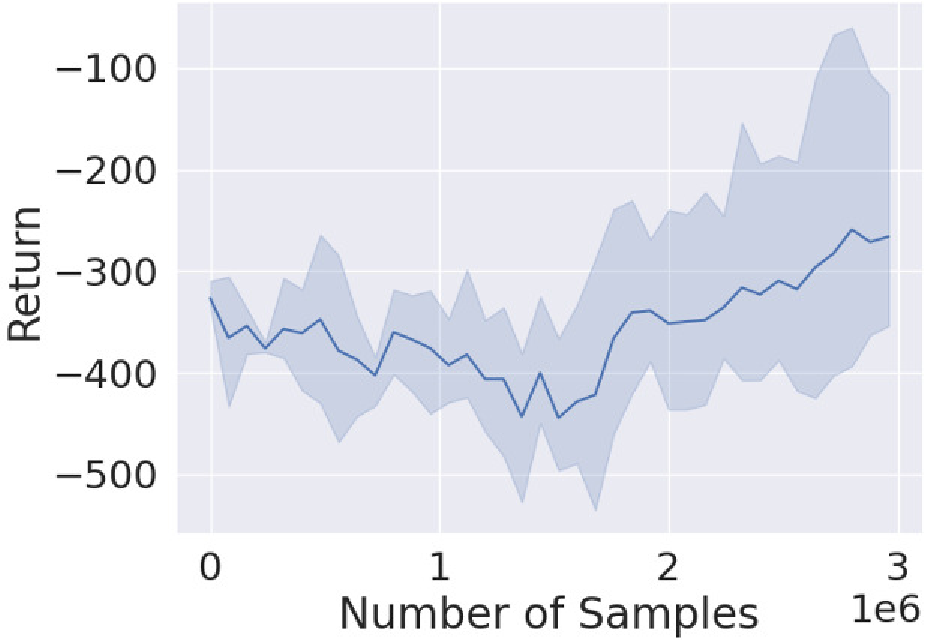
\includegraphics[width=1.5in, height=0.8in]{hc-m-exp-mz.pdf}}
\subfigure[hc-med-replay]{
\label{fig:1(b)} 
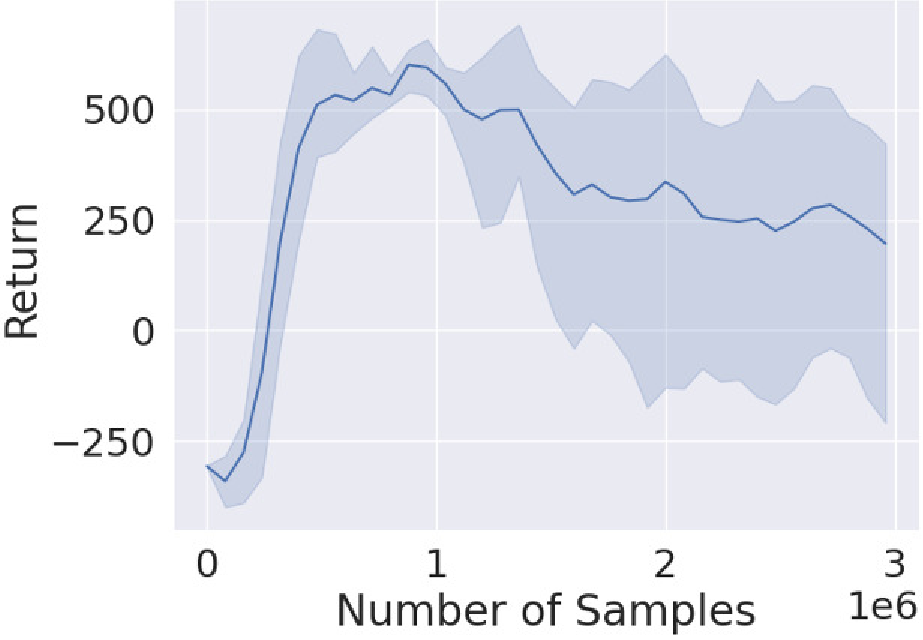
\includegraphics[width=1.5in, height=0.8in]{hc-m-rep-mz.pdf}}
\subfigure[hc-medium]{
\label{fig:1(c)} 
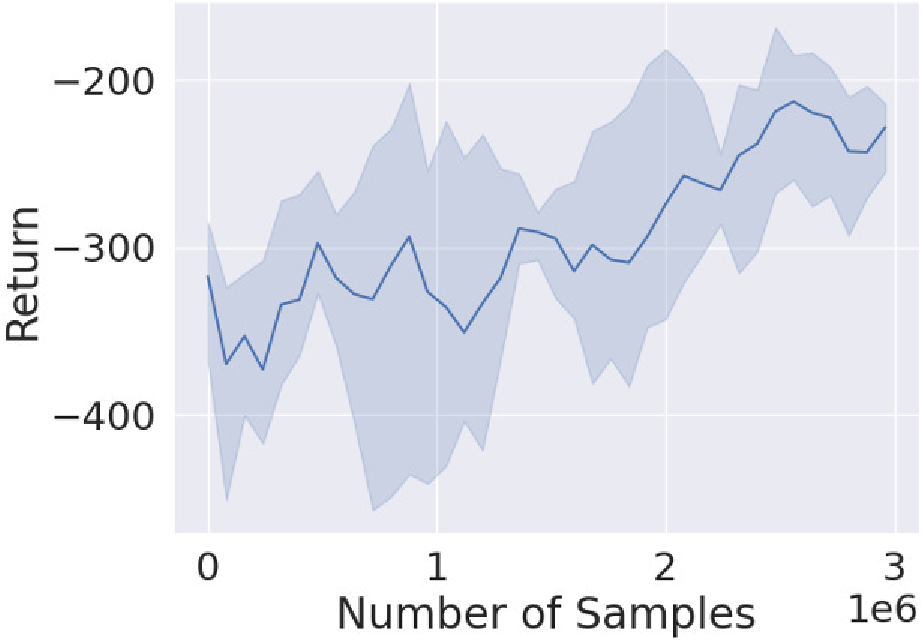
\includegraphics[width=1.5in, height=0.8in]{hc-med-mz.pdf}}
\subfigure[hc-random]{
\label{fig:1(d)} 
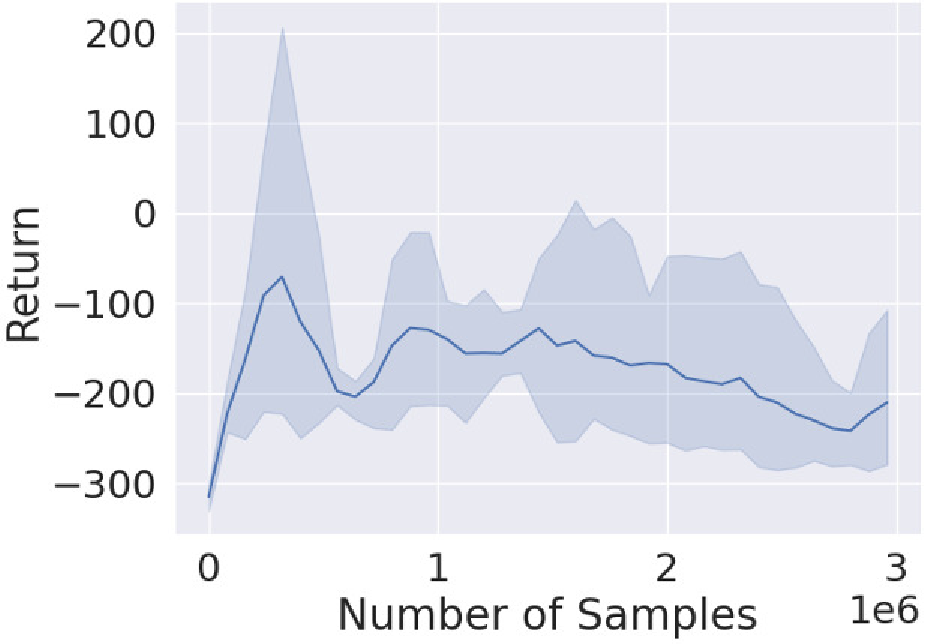
\includegraphics[width=1.5in, height=0.8in]{hc-rnd-mz.pdf}}
\subfigure[hp-med-expert]{
\label{fig:1(e)} 
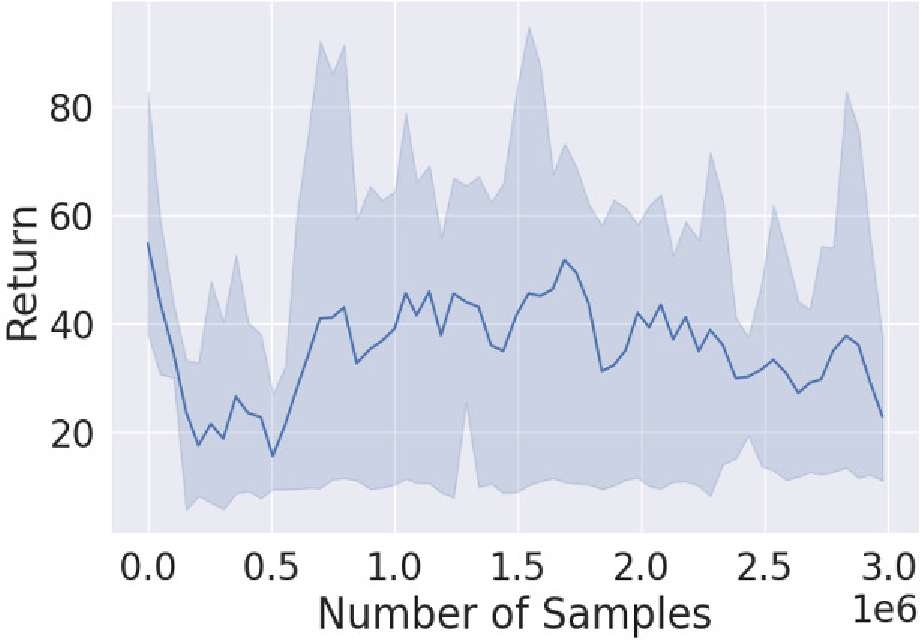
\includegraphics[width=1.5in, height=0.8in]{hp-m-exp-mz.pdf}}
\subfigure[hp-med-replay]{
\label{fig:1(f)} 
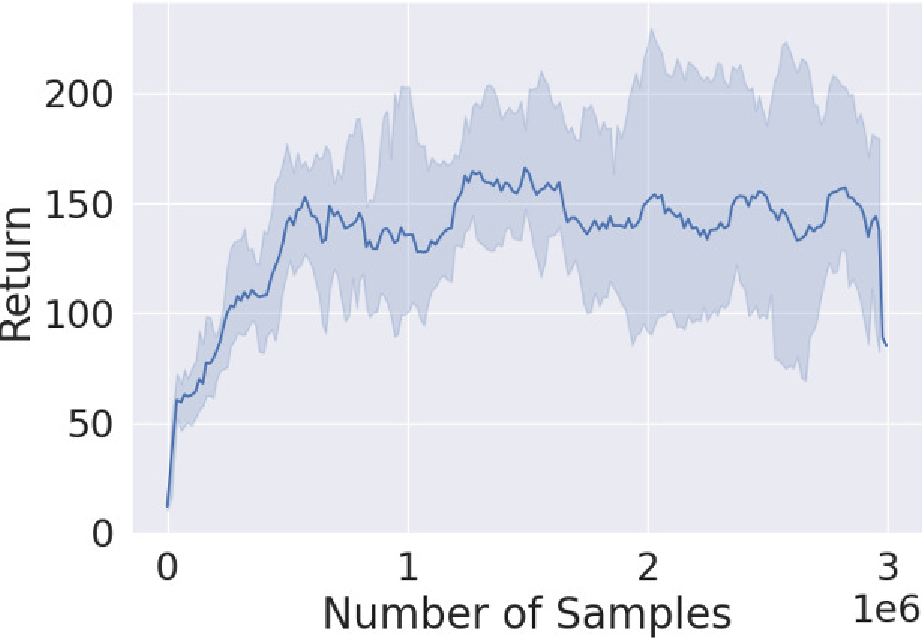
\includegraphics[width=1.5in, height=0.8in]{hp-m-rep-mz.pdf}}
\subfigure[hp-medium]{
\label{fig:1(g)} 
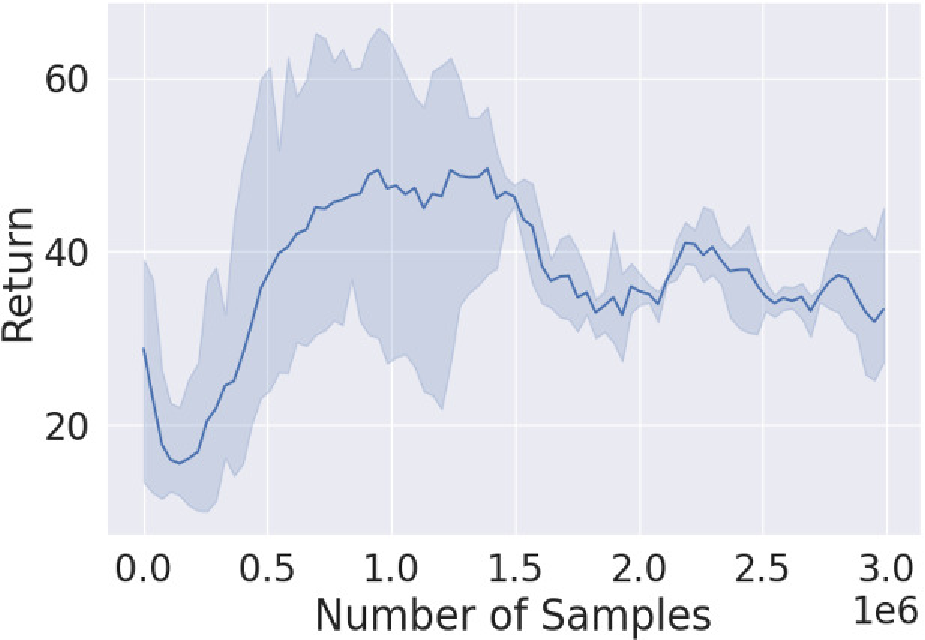
\includegraphics[width=1.5in, height=0.8in]{hp-med-mz.pdf}}
\subfigure[hp-random]{
\label{fig:1(h)} 
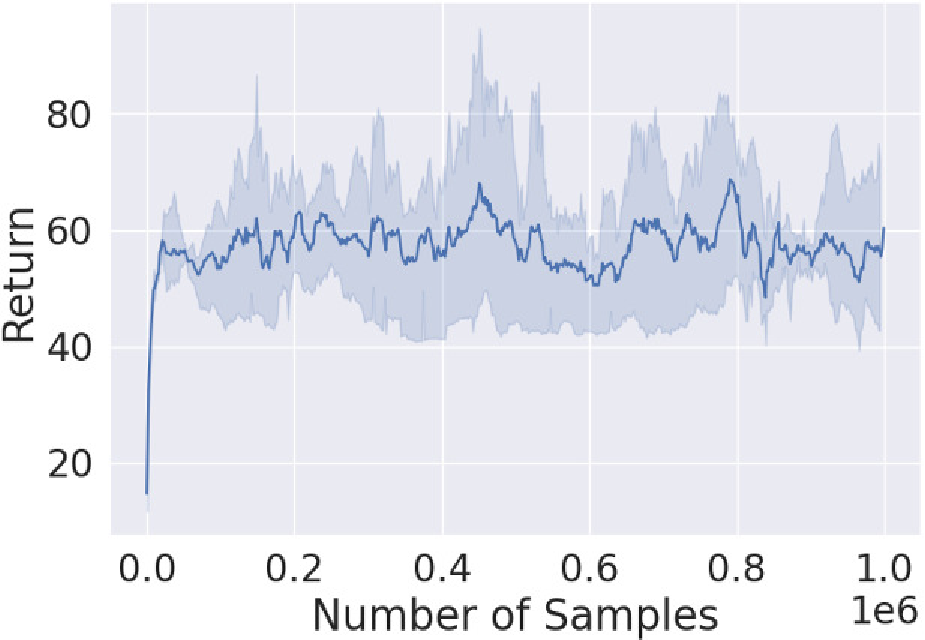
\includegraphics[width=1.5in, height=0.8in]{hp-rnd-mz.pdf}}
\subfigure[wk-med-expert]{
\label{fig:1(i)} 
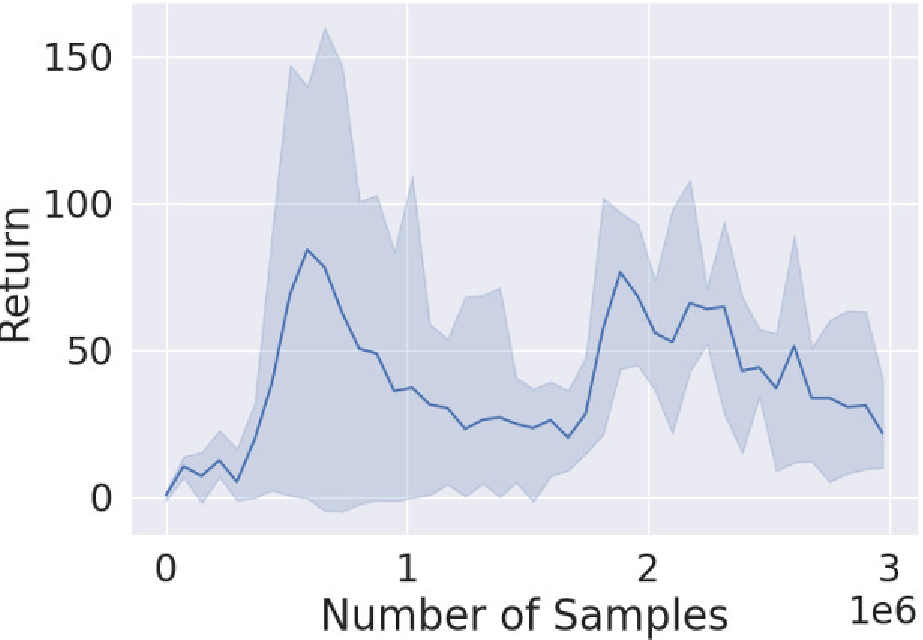
\includegraphics[width=1.5in, height=0.8in]{wk-m-exp-mz.pdf}}
\subfigure[wk-med-replay]{
\label{fig:1(j)} 
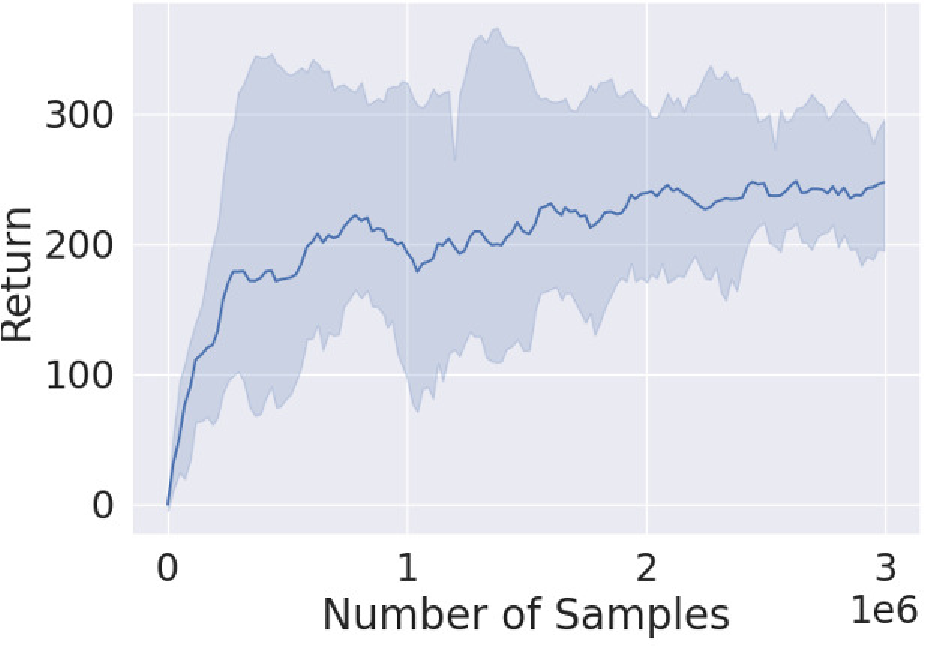
\includegraphics[width=1.5in, height=0.8in]{wk-m-rep-mz.pdf}}
\subfigure[wk-medium]{
\label{fig:1(k)} 
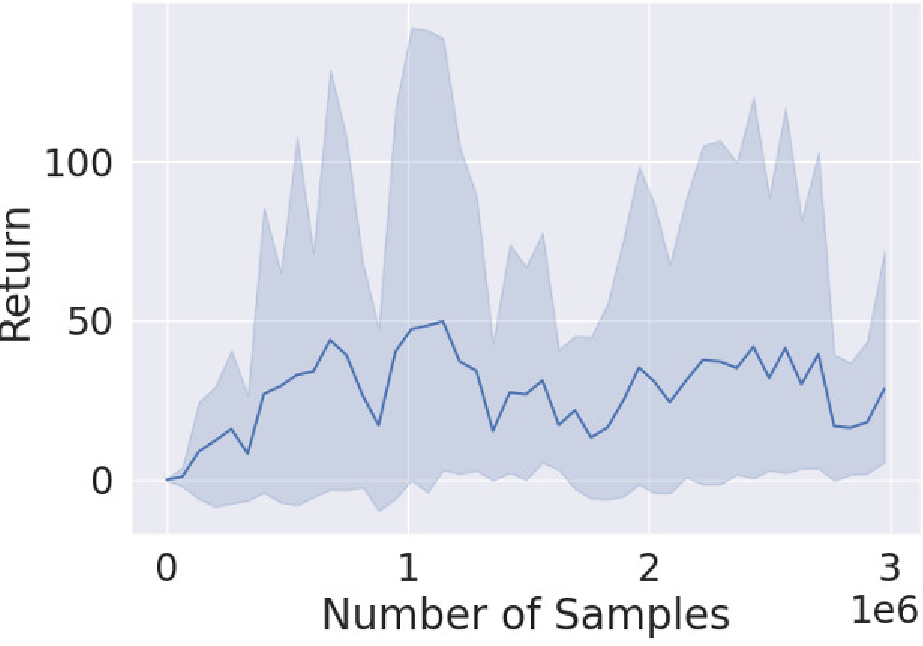
\includegraphics[width=1.5in, height=0.8in]{wk-med-mz.pdf}}
\subfigure[wk-random]{
\label{fig:1(l)} 
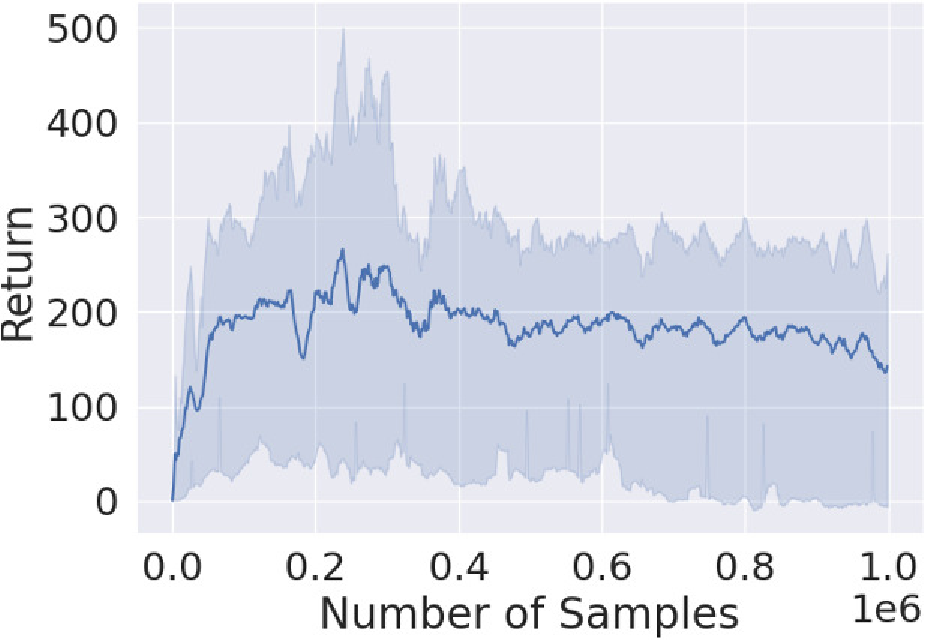
\includegraphics[width=1.5in, height=0.8in]{wk-rnd-mz.pdf}}
\caption{Performance of Sampled EfficientZero on D4RL MuJoCo tasks. The results for HalfCheetah, Hopper, and Walker2d are presented in the three rows, respectively. Each subfigure depicts the change in undiscounted episodic return as a function of the number of training samples. Experiments are repeated three times with different random seeds, with the solid line representing the mean and the shaded area indicating the 95\% confidence interval. For reference, the expert-level episodic returns for HalfCheetah, Hopper, and Walker2d are 12135, 3234.3, and 4592.3, respectively.}
\label{fig:1} 
\end{figure*}


\begin{figure}[t]
    \centering
    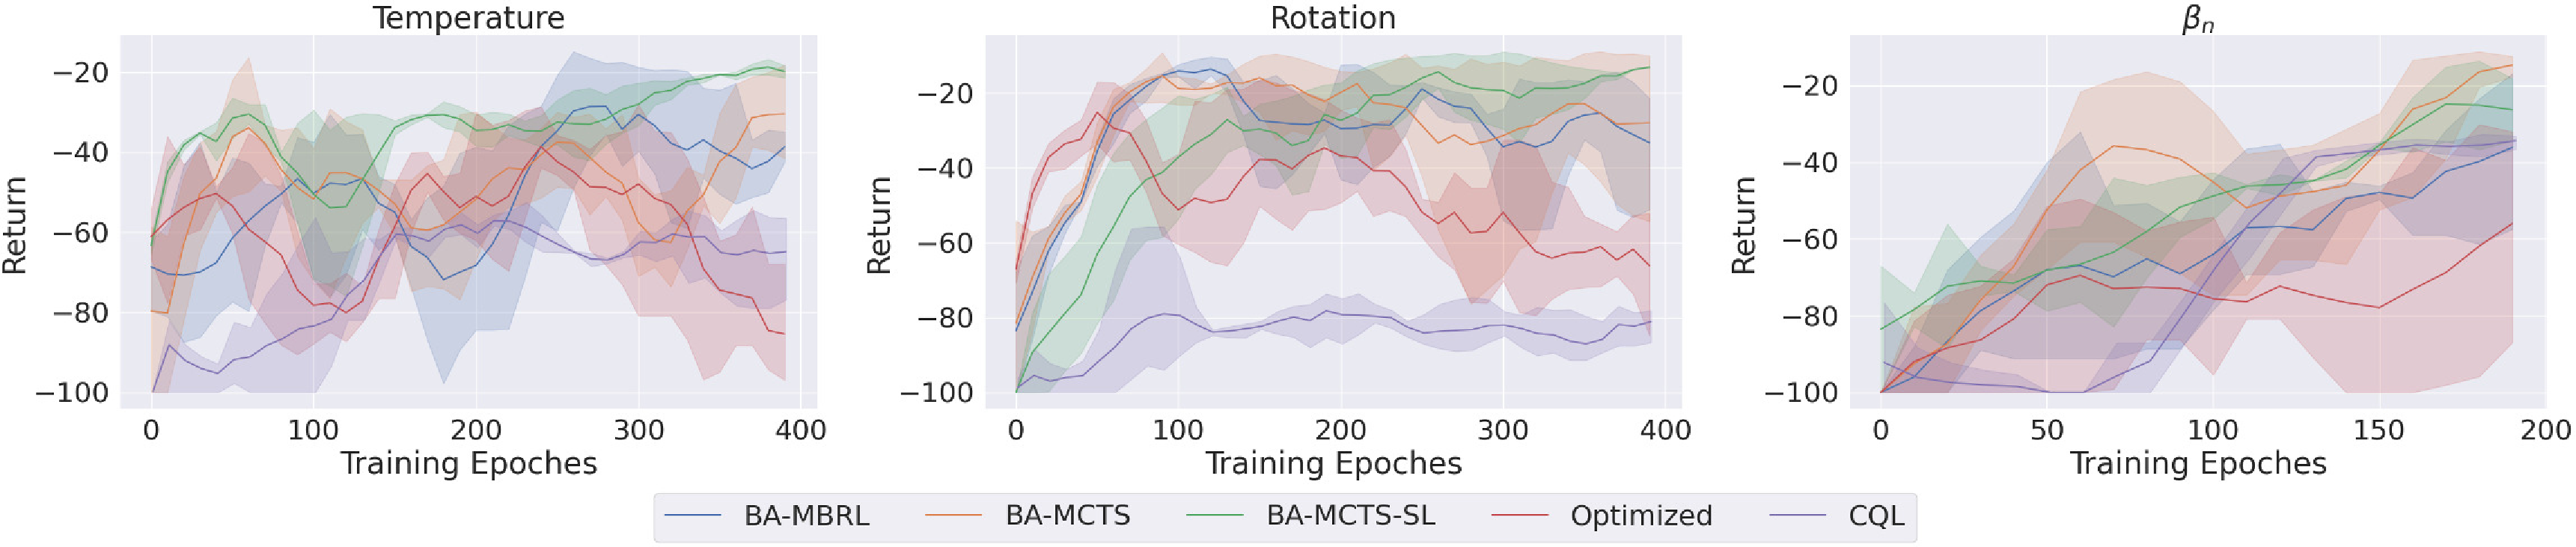
\includegraphics[width=\linewidth, height=1.5in]{nf_return-eps-converted-to.pdf} % or use height
    \caption{Evaluation results for the tokamak control tasks. The figure shows the change in episodic returns over training epochs for the proposed algorithms and baselines across three target tracking tasks in the nuclear fusion scenario. Solid lines represent the average performance, while shaded areas indicate the 95\% confidence intervals.}
    \label{fig:2}
\end{figure}

For fair comparisons and real-time execution, we do not perform test-time search and adopt the same policy architecture as the baselines, i.e., a feedforward neural network, rather than an RNN that incorporates transition history as input. These alternative designs have the potential to further improve our algorithms. For implementation, we build on the codebase of Optimized (\cite{DBLP:conf/iclr/LuBPOR22}), which thoroughly explores design choices in offline MBRL, making minimal changes to the code and hyperparameter settings\footnote{The detailed hyperparameter setups of our algorithms are provided in Appendix \ref{KeyPara}.}. Therefore, we believe the performance improvements stem from the Bayesian RL framework and deep search component. Further, both components can be seamlessly integrated with other advancements in offline MBRL, such as more accurate world model learning and improved uncertainty quantification for constructing pessimistic MDPs. 

MuZero also applies deep search to MBRL. To evaluate its performance on D4RL MuJoCo tasks, we use the open-source implementation and hyperparameter configurations of Sampled EfficientZero (\cite{DBLP:conf/nips/YeLKAG21}) provided by LightZero (\cite{DBLP:conf/nips/NiuPYLZRHLL23}). Benchmarking results from LightZero indicate that Sampled EfficientZero, equipped with a Gaussian policy, achieves the best performance on (online) MuJoCo locomotion tasks compared to other MuZero variants. To adapt Sampled EfficientZero for offline learning, we employ the reanalyse technique proposed by (\cite{DBLP:conf/nips/SchrittwieserHM21}). The evaluation results are presented in Figure \ref{fig:1}. For reference, the expert-level episodic returns (corresponding to scores of 100) for HalfCheetah, Hopper, and Walker2d are 12135, 3234.3, and 4592.3, respectively. As shown, the results are significantly worse compared to the performance of offline RL methods listed in Table \ref{table:1}, despite Sampled EfficientZero's higher computational cost (detailed in Appendix \ref{CompCost}). Notably, both Sampled EfficientZero and BA-MCTS-SL rely on supervised learning for policy improvement. However, for continuous control tasks, the agent can only sample a finite number of actions at a decision point, and the search result (e.g., $\pi_{\text{ret}}$ in Algorithm \ref{alg:2}) is a distribution over this finite set, which could be a poor approximation of the optimal action distribution. Thus, purely mimicking the search result may be less sample-efficient than policy gradient methods, as it fails to account for the continuous nature of the action space. Furthermore, world model learning is the foundation of MBRL and can be particularly challenging in \textbf{continuous control and offline learning settings}, where the state-action space is vast but training data is limited. Sampled EfficientZero integrates model learning and policy training into a single stage, which significantly increases the learning difficulty (compared to BA-MCTS-SL).

Finally, we evaluate our algorithms on three target tracking tasks in tokamak control. The tokamak is one of the most promising confinement devices for achieving controllable nuclear fusion, where the primary challenge lies in confining the plasma, i.e., an ionized gas of hydrogen isotopes, while heating it and increasing its pressure to initiate and sustain fusion reactions (\cite{1512794}). Tokamak control involves applying a series of direct actuators (e.g., neutral beam, ECH power, magnetic field) and indirect actuators (e.g., setting targets for the plasma shape and density) to confine the plasma to achieve a desired state or track a given target. This sophisticated physical process is an ideal test bed for our algorithms. Specifically, we use a well-trained data-driven dynamics model provided by \cite{DBLP:journals/corr/abs-2404-12416} as a ``ground truth" simulator for the nuclear fusion process during evaluation, and generate a dataset containing 725270 transitions using this model for offline RL. We select a reference shot (i.e., an episode of a fusion process) from DIII-D\footnote{DIII-D is a tokamak device located in San Diego, California, operated by General Atomics.}, and use its trajectories of Ion Rotation, Electron Temperature, and $\beta_n$ as targets for three tracking tasks. These are critical quantities in tokamak control, particularly $\beta_n$, which serves as an economic indicator of the efficiency of nuclear fusion. The tracking tasks have a 28-dimensional state space and a 14-dimensional action space, both continuous. Moreover, these tasks are \textbf{highly stochastic}, as the underlying dynamics model is a probabilistic neural network and each state transition is a sample from this model. For details on the simulator, and the design of the state/action spaces and reward functions, please refer to Appendix \ref{DetTCT}. We compare our algorithms with SOTA model-free and model-based offline RL methods, specifically CQL and Optimized. The learning performance on the three tracking tasks is shown in Figure \ref{fig:2}, where the x-axis and y-axis represent the training epochs and (negative) full-shot tracking errors, respectively. Our algorithms consistently outperform the baselines. Notably, the offline dataset does not include the reference shot or any similar, nearby shots. Therefore, restricting the policy to stay close to the behavior policy, as done in model-free methods, can be problematic. Also, learning dynamics models for MBRL is quite challenging in this nuclear fusion scenario. Our algorithms share the same ensemble of dynamics models with ``Optimized" for policy learning, and the comparisons can demonstrate the superiority of Bayesian RL and deep search. Figure \ref{fig:2} has been smoothed for visualization\footnote{The episodic return is plotted every 10 training epochs, with the y-axis representing the average value of a sliding window of length 5.}. We further report the average return over the final 10 training epochs in Table \ref{table:6}, and the conclusions align with those from the D4RL MuJoCo tasks, showing the robustness of our proposed algorithms.

\begin{table}[t]
\small
\centering
\begin{tabular}{c|c|c|c|c|c}
\hline
{Task} & {\makecell{BA-MCTS \\ -SL (ours)}} & {\makecell{BA-MCTS \\ (ours)}} & {\makecell{BA-MBRL \\ (ours)}} & {CQL} & {Optimized}\\
\hline 
\hline
{Temperature} & {\textbf{-21.16} $\pm$ 5.00} & {-23.83 $\pm$ 9.66} & {-29.35 $\pm$ 4.72} & {-59.62 $\pm$ 1.57} & {-83.55 $\pm$ 10.56} \\
{Rotation} & {\textbf{-14.14} $\pm$ 1.88} & {-19.07 $\pm$ 5.85} & {-31.33 $\pm$ 11.54} & {-85.48 $\pm$ 2.72} & {-71.54 $\pm$ 9.88} \\
{$\beta_{n}$} & {-37.03 $\pm$ 17.98} & {\textbf{-18.93} $\pm$ 1.75} & {-23.4 $\pm$ 10.77} & {-36.37 $\pm$ 1.17} & {-57.84 $\pm$ 10.27} \\
\hline
\hline
{Average} & {-24.11} & {\textbf{-20.61}} & {-28.03} & {-60.49} & {-70.98} \\
\hline 
\end{tabular}
\caption{Comparisons between the proposed algorithms and offline RL baselines on the target tracking tasks. For each algorithm, we report the average return of the final ten policy learning epochs and its standard deviation across three different random seeds.}
\label{table:6}
\end{table}

 % get rid of implementation tricks, do minimal changes, see the improvement brought by the search component. 

 % muzero fails, learning dyn and policy at the same stage can be very challenging, especially for complex continuous control tasks

\section{Conclusion}
In this work, we advance the method of {machine unlearning} through a novel viewpoint: model sparsification, achieved by weight pruning. We show in both theory and practice that model sparsity plays a foundational and crucial role in closing the gap between exact unlearning and existing approximate unlearning methods. Inspired by that, we propose two new unlearning paradigms,  `prune first, then unlearn' and `sparsity-aware unlearn', which can significantly improve the efficacy of approximate unlearning. We demonstrate the effectiveness of our findings and proposals in extensive experiments across different unlearning setups. Our study also indicates the presence of \textit{model modularity} traits, such as weight sparsity, that could simplify the process of machine unlearning. This may open up exciting prospects for future research to investigate unlearning patterns within weight or architecture space.






\bibliography{main}
\bibliographystyle{tmlr}

\newpage


% \setcounter{lemma}{0}
%     \renewcommand{\thelemma}{\Alph{section}\arabic{lemma}}
    
\begin{comment}
\end{comment}

{\colorred 
\section{Compatible Value Function}
\label{app:comp_v}

The original policy gradient with compatible value function is stated as follow. 
\begin{theorem}
[\cite{sutton1999policy}]
Let $Q_w$ be a state-action function with parameter $w$ and $\pi_\theta$ be a policy function with parameter $\theta$. 
If $Q_w$ satisfies $\mathbb{E}_{\pi} [(Q^\pi - Q_w) \nabla_w Q_w] = 0$ and 
$\nabla_w Q_w = \nabla_\theta \log \pi_\theta,$
then $$\nabla_\theta \mathcal{J} = \mathbb{E}_\pi [Q_w \nabla_\theta \log \pi_\theta].$$
\label{thm:pg_fa}
\end{theorem}
If we let $w = \theta$ in Theorem \ref{thm:pg_fa}, where $Q_w$ and $\pi_\theta$ share parameters, we have the following theorem. 
\begin{theorem}
Let $Q_\theta$ be a state-action function with parameter $\theta$ and $\pi_\theta$ be a policy function with parameter $\theta$. 
If $Q_\theta$ satisfies $\mathbb{E}_{\pi} [(Q^\pi - Q_\theta) \nabla_\theta Q_\theta] = 0$ and 
$\nabla_\theta Q_\theta = \nabla_\theta \log \pi_\theta,$
then $$\nabla_\theta \mathcal{J} = \mathbb{E}_\pi [Q_\theta \nabla_\theta \log \pi_\theta].$$
\label{thm:pg_fa2}
\end{theorem}
Define 
$$\chi \overset{def}{=} \mathbb{E}_\pi [\cos <\nabla_\theta Q_\theta, \nabla_\theta \log \pi_\theta>].$$
We show that $\chi = 1$ is the necessary condition for the compatible condition $\nabla_\theta Q_\theta = \nabla_\theta \log \pi_\theta$. 
\begin{theorem}
i) If $\nabla_\theta Q_\theta \propto \nabla_\theta \log \pi_\theta$ for all states, then $\chi = 1$.

ii) If $\chi = 1$, then $\nabla_\theta Q_\theta \propto \nabla_\theta \log \pi_\theta$ for all states. 
\label{thm:connect_cond}
\end{theorem}
By Theorem \ref{thm:connect_cond}, $\chi = 1$ is equivalent to $\nabla_\theta Q_\theta \propto \nabla_\theta \log \pi_\theta$, and $\nabla_\theta Q_\theta \propto \nabla_\theta \log \pi_\theta$ is the necessary condition for $\nabla_\theta Q_\theta = \nabla_\theta \log \pi_\theta$, hence $\chi = 1$ is the necessary condition for $\nabla_\theta Q_\theta = \nabla_\theta \log \pi_\theta$.
\begin{proof}
i) Since $\nabla_\theta Q_\theta \propto \nabla_\theta \log \pi_\theta$, we have $<\nabla_\theta Q_\theta, \nabla_\theta \log \pi_\theta> = 0$. 
By definition of $\chi$, we have 
$$\chi = \mathbb{E}_\pi [\cos <\nabla_\theta Q_\theta, \nabla_\theta \log \pi_\theta>] = \mathbb{E}_\pi [1] = 1.$$

ii) Since $\chi \leq 1$ and $\cos(x)$ is monotonic decreasing as $x$ goes from $0$ to $\pi$, the equality $\chi = 1$ only holds when all states satisfy $\cos <\nabla_\theta Q_\theta, \nabla_\theta \log \pi_\theta> = 0$, which means $\nabla_\theta Q_\theta \propto \nabla_\theta \log \pi_\theta$. 
\end{proof}
}

% $$
% \begin{aligned}
%     logp &= variable((3, 3, 4)) \\
%     q &= variable((3, 3, 4)) \\
%     alpha &= 0.3 \\
%     \pi &= softmax(alpha * logp + (1.0 - alpha) * q) \\
% \end{aligned}
% $$
\clearpage

\section{Gradients Between Policy Improvement and Policy Evaluation}
\label{app:mtv}

\begin{table}[hb!]
    \centering
    \scalebox{0.90}{
    \begin{math}
        \begin{array}{c|c|c|c}
    \toprule
     & \text{Function Approximation} & \text{Train Gradients} & \text{Cosine of Interested Angles} \\
    \midrule
    
    \text{PPO} & (V, logit) = (V_\theta, logit_\theta) & 0.5 \nabla L_V + \nabla \mathcal{J} & %\cos<\nabla L_V, \nabla \mathcal{J}> 
    \\ 
    & \pi = \text{softmax}(logit) & & \\
    
    \midrule
    
    \text{PPO ver.1} & (Q, logit) = (Q_\theta, logit_\theta), & 0.5 \nabla L_V + \nabla \mathcal{J} & \cos<\nabla L_Q, \nabla \mathcal{J}>%\cos<\nabla L_V, \nabla \mathcal{J}> 
    \\
    & \pi = \text{softmax}(logit) & & \cos<\nabla Q, \nabla \log \pi> \\
    & V = sg(\pi)\cdot Q & & %\cos<\nabla L_V, \nabla L_Q> 
    \\
    % & & &  \\
    
    \midrule
    
    \text{PPO ver.2} & (Q, logit) = (Q_\theta, logit_\theta), & 0.5 \nabla L_V + \nabla L_Q + \nabla \mathcal{J} & \cos<\nabla L_Q, \nabla \mathcal{J}> %\cos<\nabla L_V, \nabla \mathcal{J}> 
    \\
    & pi = \text{softmax}(logit) & & \cos<\nabla Q, \nabla \log \pi> \\
    & V = sg(\pi)\cdot Q & & %\cos<\nabla L_V, \nabla L_Q> 
    \\
    % & & &  \\
    
    \midrule
    
    \text{PPO+CASA} & (V, A) = (V_\theta, A_\theta), & 0.5 \nabla L_V + \nabla L_Q + \nabla \mathcal{J} & \cos<\nabla L_Q, \nabla \mathcal{J}> %\cos<\nabla L_V, \nabla \mathcal{J}> 
    \\
    & \pi = \text{softmax}(A/\tau), & & \cos<\nabla Q, \nabla \log \pi> \\
    & \Bar{A} = A - sg(\pi) \cdot A & & %\cos<\nabla L_V, \nabla L_Q> 
    \\
    & Q = \Bar{A} + sg(V) & &  \\
    
    \bottomrule 
    \end{array}
    \end{math}
    }
    
    \caption{PPO is the original PPO. PPO ver.1 and PPO ver.2 are adapted versions to calculate $\nabla L_Q$. PPO+CASA is applying CASA on PPO, which is described in Sec. \ref{sec:on_ppo_and_r2d2}.}
    \label{tab:ppo_mtv}
\end{table}

\begin{table}[ht!]
    \centering
    \scalebox{0.90}{
    \begin{math}
        \begin{array}{c|c|c|c}
    \toprule
     & \text{Function Approximation} & \text{Train Gradients} & \text{Cosine of Interested Angles} \\
    \midrule
    
    \text{R2D2} & (V, A) = (V_\theta, A_\theta) & \nabla L_Q & \cos<\nabla L_Q, \nabla \mathcal{J}>  %\cos<\nabla L_V, \nabla \mathcal{J}> 
    \\
    & Q = A + V & & \\
    & \pi = \text{softmax}(A / \tau) & & %\cos<\nabla L_V, \nabla L_Q> 
    \\
    % & & &  \\ % <\nabla Q, \nabla \log \pi>

    \midrule
    
    \text{R2D2 ver.1} & (V, A) = (V_\theta, A_\theta) & 0.5 \nabla L_V + \nabla L_Q & \cos<\nabla L_Q, \nabla \mathcal{J}>  % \cos<\nabla L_V, \nabla \mathcal{J}> 
    \\
    & Q = A + V & & % \cos<\nabla L_Q, \nabla \mathcal{J}> 
    \\
    & \pi = \text{softmax}(A / \tau) & & % \cos<\nabla L_V, \nabla L_Q> 
    \\
    % & & &  \\ % \cos<\nabla Q, \nabla \log \pi>

    \midrule
    
    \text{R2D2+CASA} & (V, A) = (V_\theta, A_\theta), & 0.5 \nabla L_V + \nabla L_Q + \nabla \mathcal{J} & \cos<\nabla L_Q, \nabla \mathcal{J}>  % \cos<\nabla L_V, \nabla \mathcal{J}> 
    \\
    & \pi = \text{softmax}(A/\tau),  & & %\cos<\nabla L_Q, \nabla \mathcal{J}> 
    \\
    & \Bar{A} = A - sg(\pi) \cdot A & & % \cos<\nabla L_V, \nabla L_Q> 
    \\
    & Q = \Bar{A} + sg(V) & &  \\ %\cos<\nabla Q, \nabla \log \pi>
    \bottomrule 
    \end{array}
    \end{math}
     }
    \caption{R2D2 is the original R2D2. R2D2 ver.1 is adapted version to include $\nabla L_V$ for training. R2D2+CASA is applying CASA on R2D2, which is described in Sec. \ref{sec:on_ppo_and_r2d2}.}
    \label{tab:r2d2_mtv}
\end{table}

To understand the behavior of 
{\colorred $$
    \beta \overset{def}{=} <\mathbb{E}_\pi[(Q^\pi-Q_\theta)\nabla_\theta Q_\theta],\, \mathbb{E}_\pi[(Q^\pi-V_\theta) \nabla_\theta \log \pi_\theta]>
$$
}
and 
{\colorred 
$$\chi \overset{def}{=} \mathbb{E}_\pi [\cos <\nabla_\theta Q_\theta, \nabla_\theta \log \pi_\theta>]$$
}
in reinforcement learning algorithms, we choose PPO as a representative for policy-based methods and R2D2 as a representative for value-based algorithms. 

Define $$L_V(\theta) = \mathbb{E}_\pi [ (V^{\pi} - V_\theta)^2 ],\  L_Q(\theta) = \mathbb{E}_\pi [ (Q^{\pi} - Q_\theta)^2 ],$$
and $$\nabla_\theta \mathcal{J}(\theta) = \mathbb{E}_\pi \left[ (Q^{\pi}  - V_\theta ) \nabla_\theta \log \pi \right].$$
We usually have above three kinds of loss functions in reinforcement learning, which aim to estimate the state values, state-action values and the policy. 
We do not talk about the estimations of $V^\pi$ and $Q^\pi$ as they are estimated as their usual way of PPO's and R2D2's. 
All hyperparameters are listed in Appendix \ref{app:hyperparameters}. 

{\colorred For brevity, we write 
$$\cos<\nabla Q, \nabla \log \pi> = \mathbb{E}_\pi [\cos <\nabla_\theta Q_\theta, \nabla_\theta \log \pi_\theta>],$$
and
$$
\begin{aligned}
    &\cos<\nabla L_Q, \nabla \mathcal{J}> = \cos<\mathbb{E}_\pi[(Q^\pi-Q_\theta)\nabla_\theta Q_\theta],\, \mathbb{E}_\pi[(Q^\pi-V_\theta) \nabla_\theta \log \pi_\theta]>, \\
    &\cos<\nabla L_V, \nabla \mathcal{J}> = \cos<\mathbb{E}_\pi[(V^\pi-V_\theta)\nabla_\theta V_\theta],\, \mathbb{E}_\pi[(Q^\pi-V_\theta) \nabla_\theta \log \pi_\theta]>, \\
    &\cos<\nabla L_V, \nabla L_Q> = \cos<\mathbb{E}_\pi[(V^\pi-V_\theta)\nabla_\theta V_\theta],\, \mathbb{E}_\pi[(Q^\pi-Q_\theta) \nabla_\theta Q_\theta]>. \\
\end{aligned}
$$}

The fact that PPO only has $\nabla_\theta L_V$ and $\nabla_\theta \mathcal{J}$ and R2D2 only has $\nabla_\theta L_Q$ is the main difficulty to track $\cos(\beta)$ and $\chi$. 
To solve the problem, we adjust PPO and R2D2 with different versions.

For PPO, we displace the estimation of $V_\theta$ by $sg(\pi)\cdot Q_\theta$, where $Q_\theta$ is estimated by function approximation and $V_\theta$ is estimated by taking the expectation of $Q_\theta$.
All versions of PPO are listed in Table \ref{tab:ppo_mtv}.

For R2D2, we point out that though we apply $\epsilon$-greedy to interact with environments, $\epsilon$ is only used for exploration and the final target policy of value-based methods is simply $\arg\max Q_\theta$. 
Because $\arg\max Q_\theta$ breaks the gradient, we use a surrogate policy to approximate the gradient of policy improvement. 
% \haosen{potential context, the necessity of measuring the policy gradient and ``entropy'' of the Q function is that R2D2's greedy policy changes rapidly, and the rapid change give R2D2 the implicit exploration ability. \citep{policychurn} }
Since R2D2 uses dueling structure and $\text{softmax}(A_\theta / \tau) = \text{softmax}(Q_\theta / \tau) \overset{\tau \rightarrow 0+}{\longrightarrow} \arg\max Q_\theta$, we use $\pi_{surrogate} = \text{softmax}(A_\theta / \tau)$ to calculate the policy gradient. 
We only use $\pi_{surrogate}$ on learner to calculate the gradient, where the policy that interacts with environments is still $\epsilon$-greedy. 
All versions of R2D2 are listed in Table \ref{tab:r2d2_mtv}.

% Results are shown in Figure \ref{fig:mtv_app}.


% \begin{figure}[hb!]
% % \centering
% 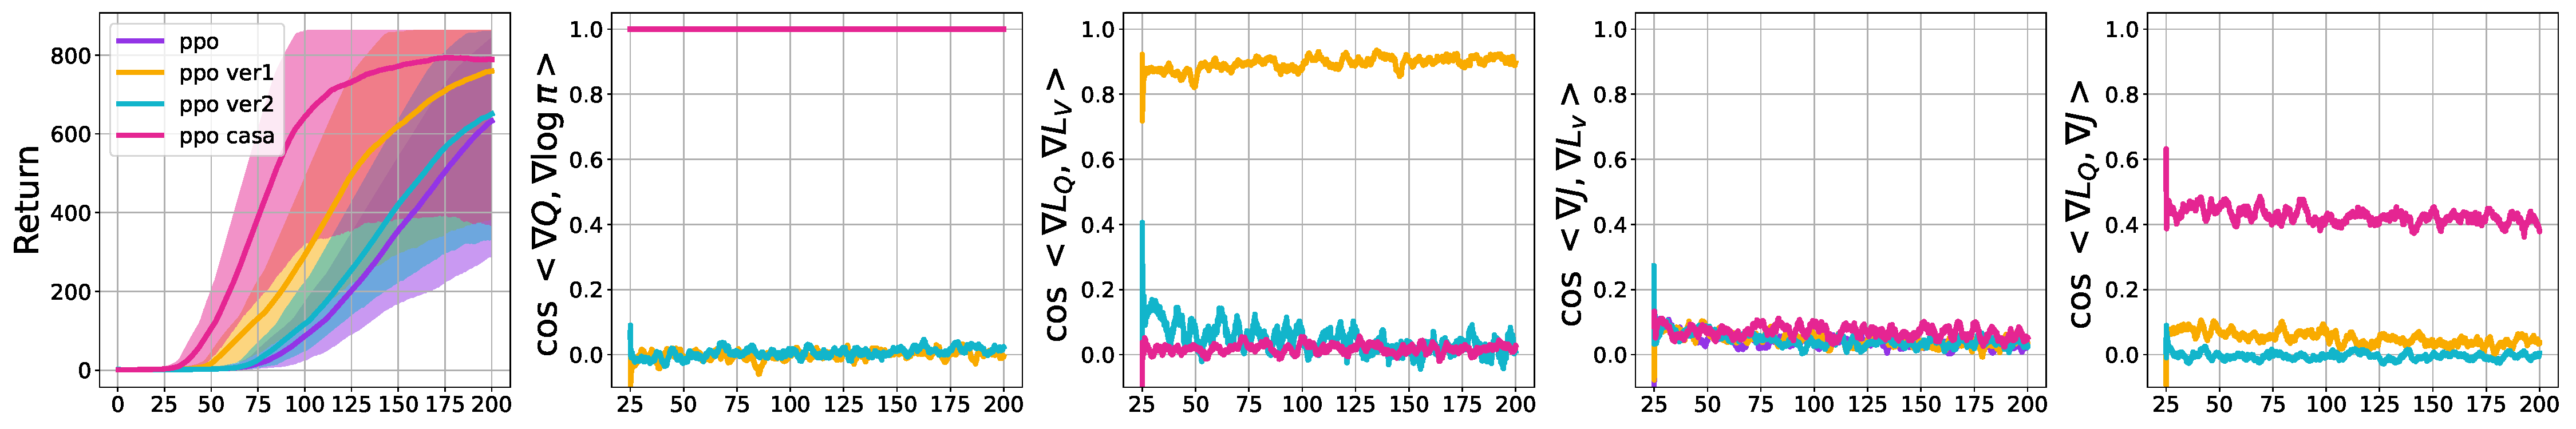
\includegraphics[width=\linewidth]{body/app_fig/app_ppo_Breakout.pdf}

% 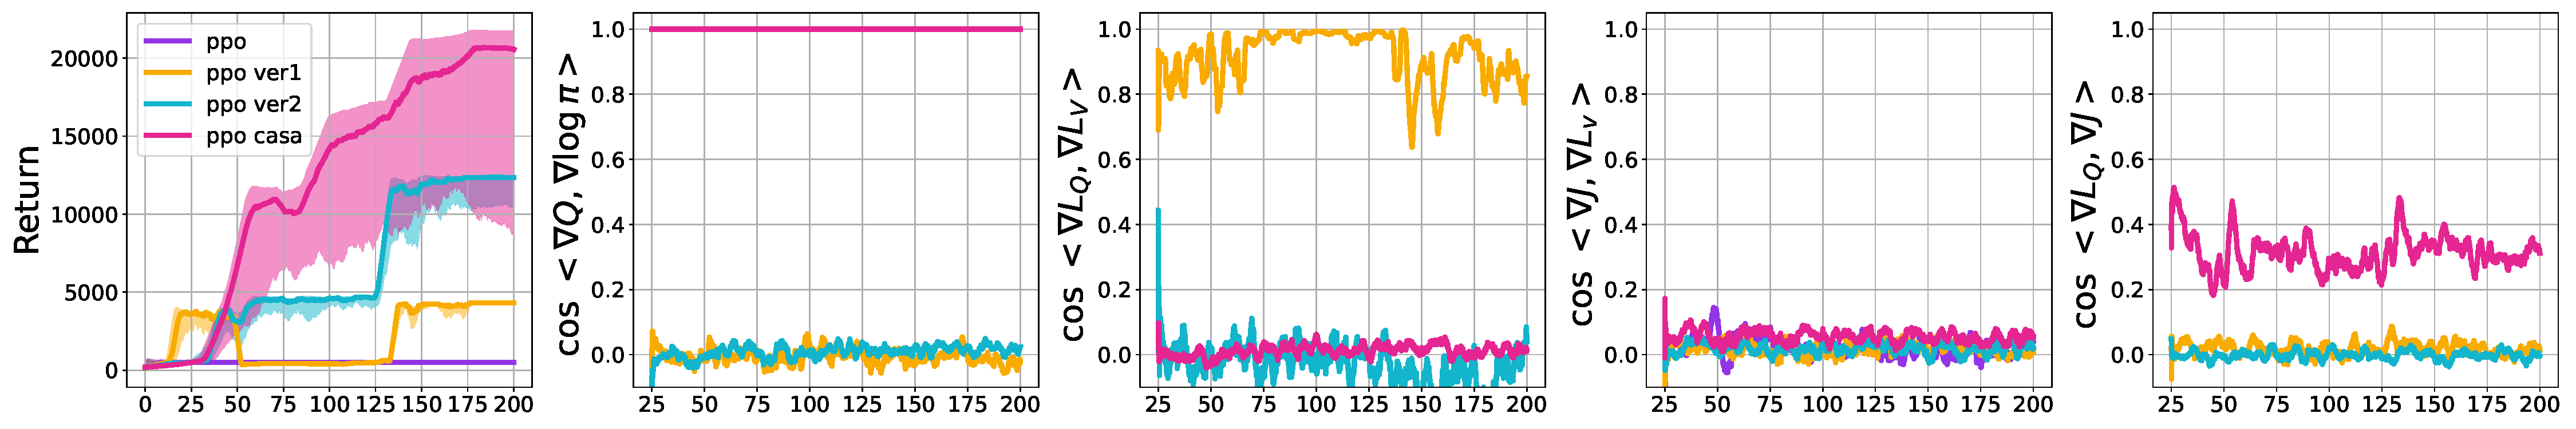
\includegraphics[width=\linewidth]{body/app_fig/app_ppo_Qbert.pdf}

% 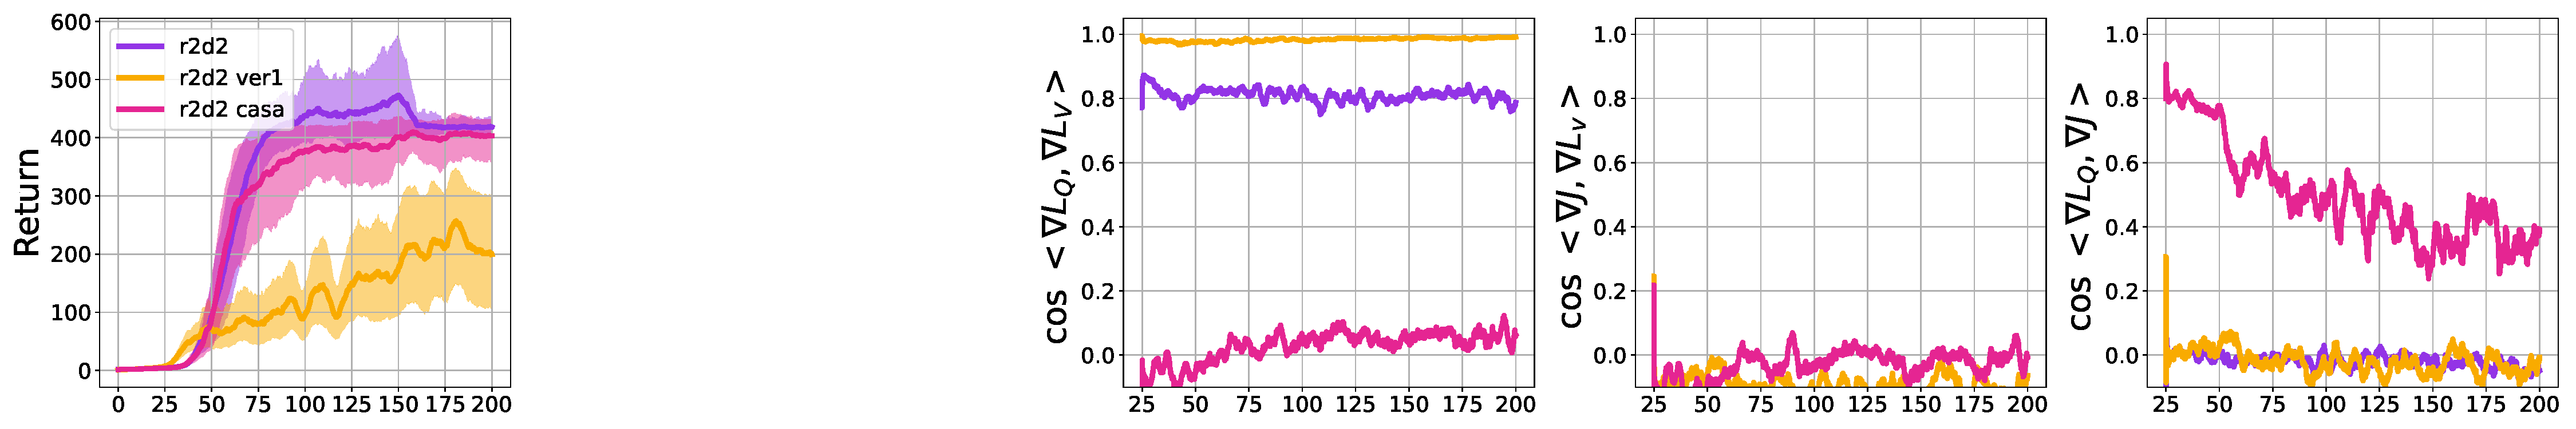
\includegraphics[width=\linewidth]{body/app_fig/app_r2d2_Breakout.pdf}


% 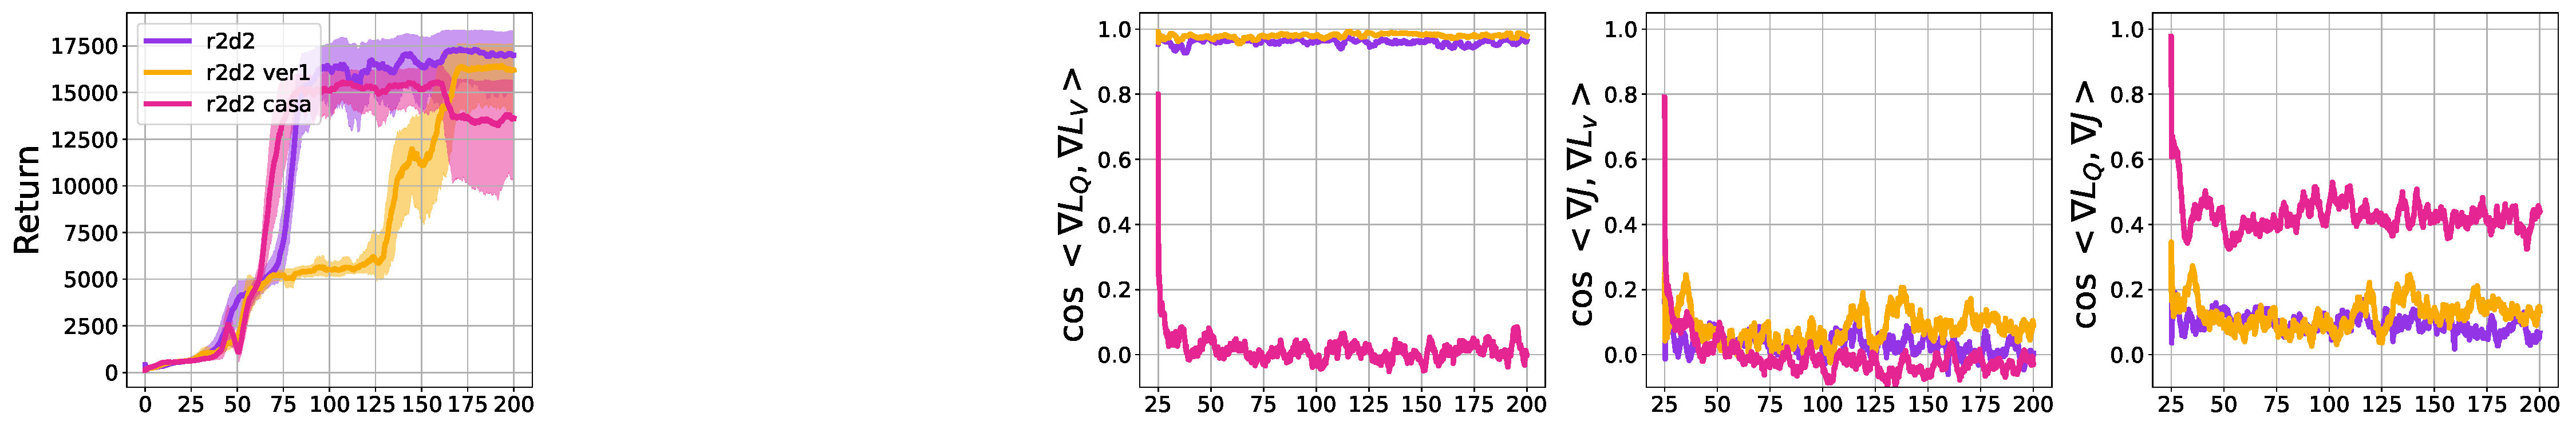
\includegraphics[width=\linewidth]{body/app_fig/app_r2d2_Qbert.pdf}
% \caption{Angles of Gradients and Returns of versions of PPO and R2D2 defined in Table \ref{tab:ppo_mtv} and Table \ref{tab:r2d2_mtv}.}
% \label{fig:mtv_app}
% \end{figure}

% \clearpage

% \changnan{casa summary deleted}
% \section{CASA summary}
% \begin{figure}[ht]
% \centering
% 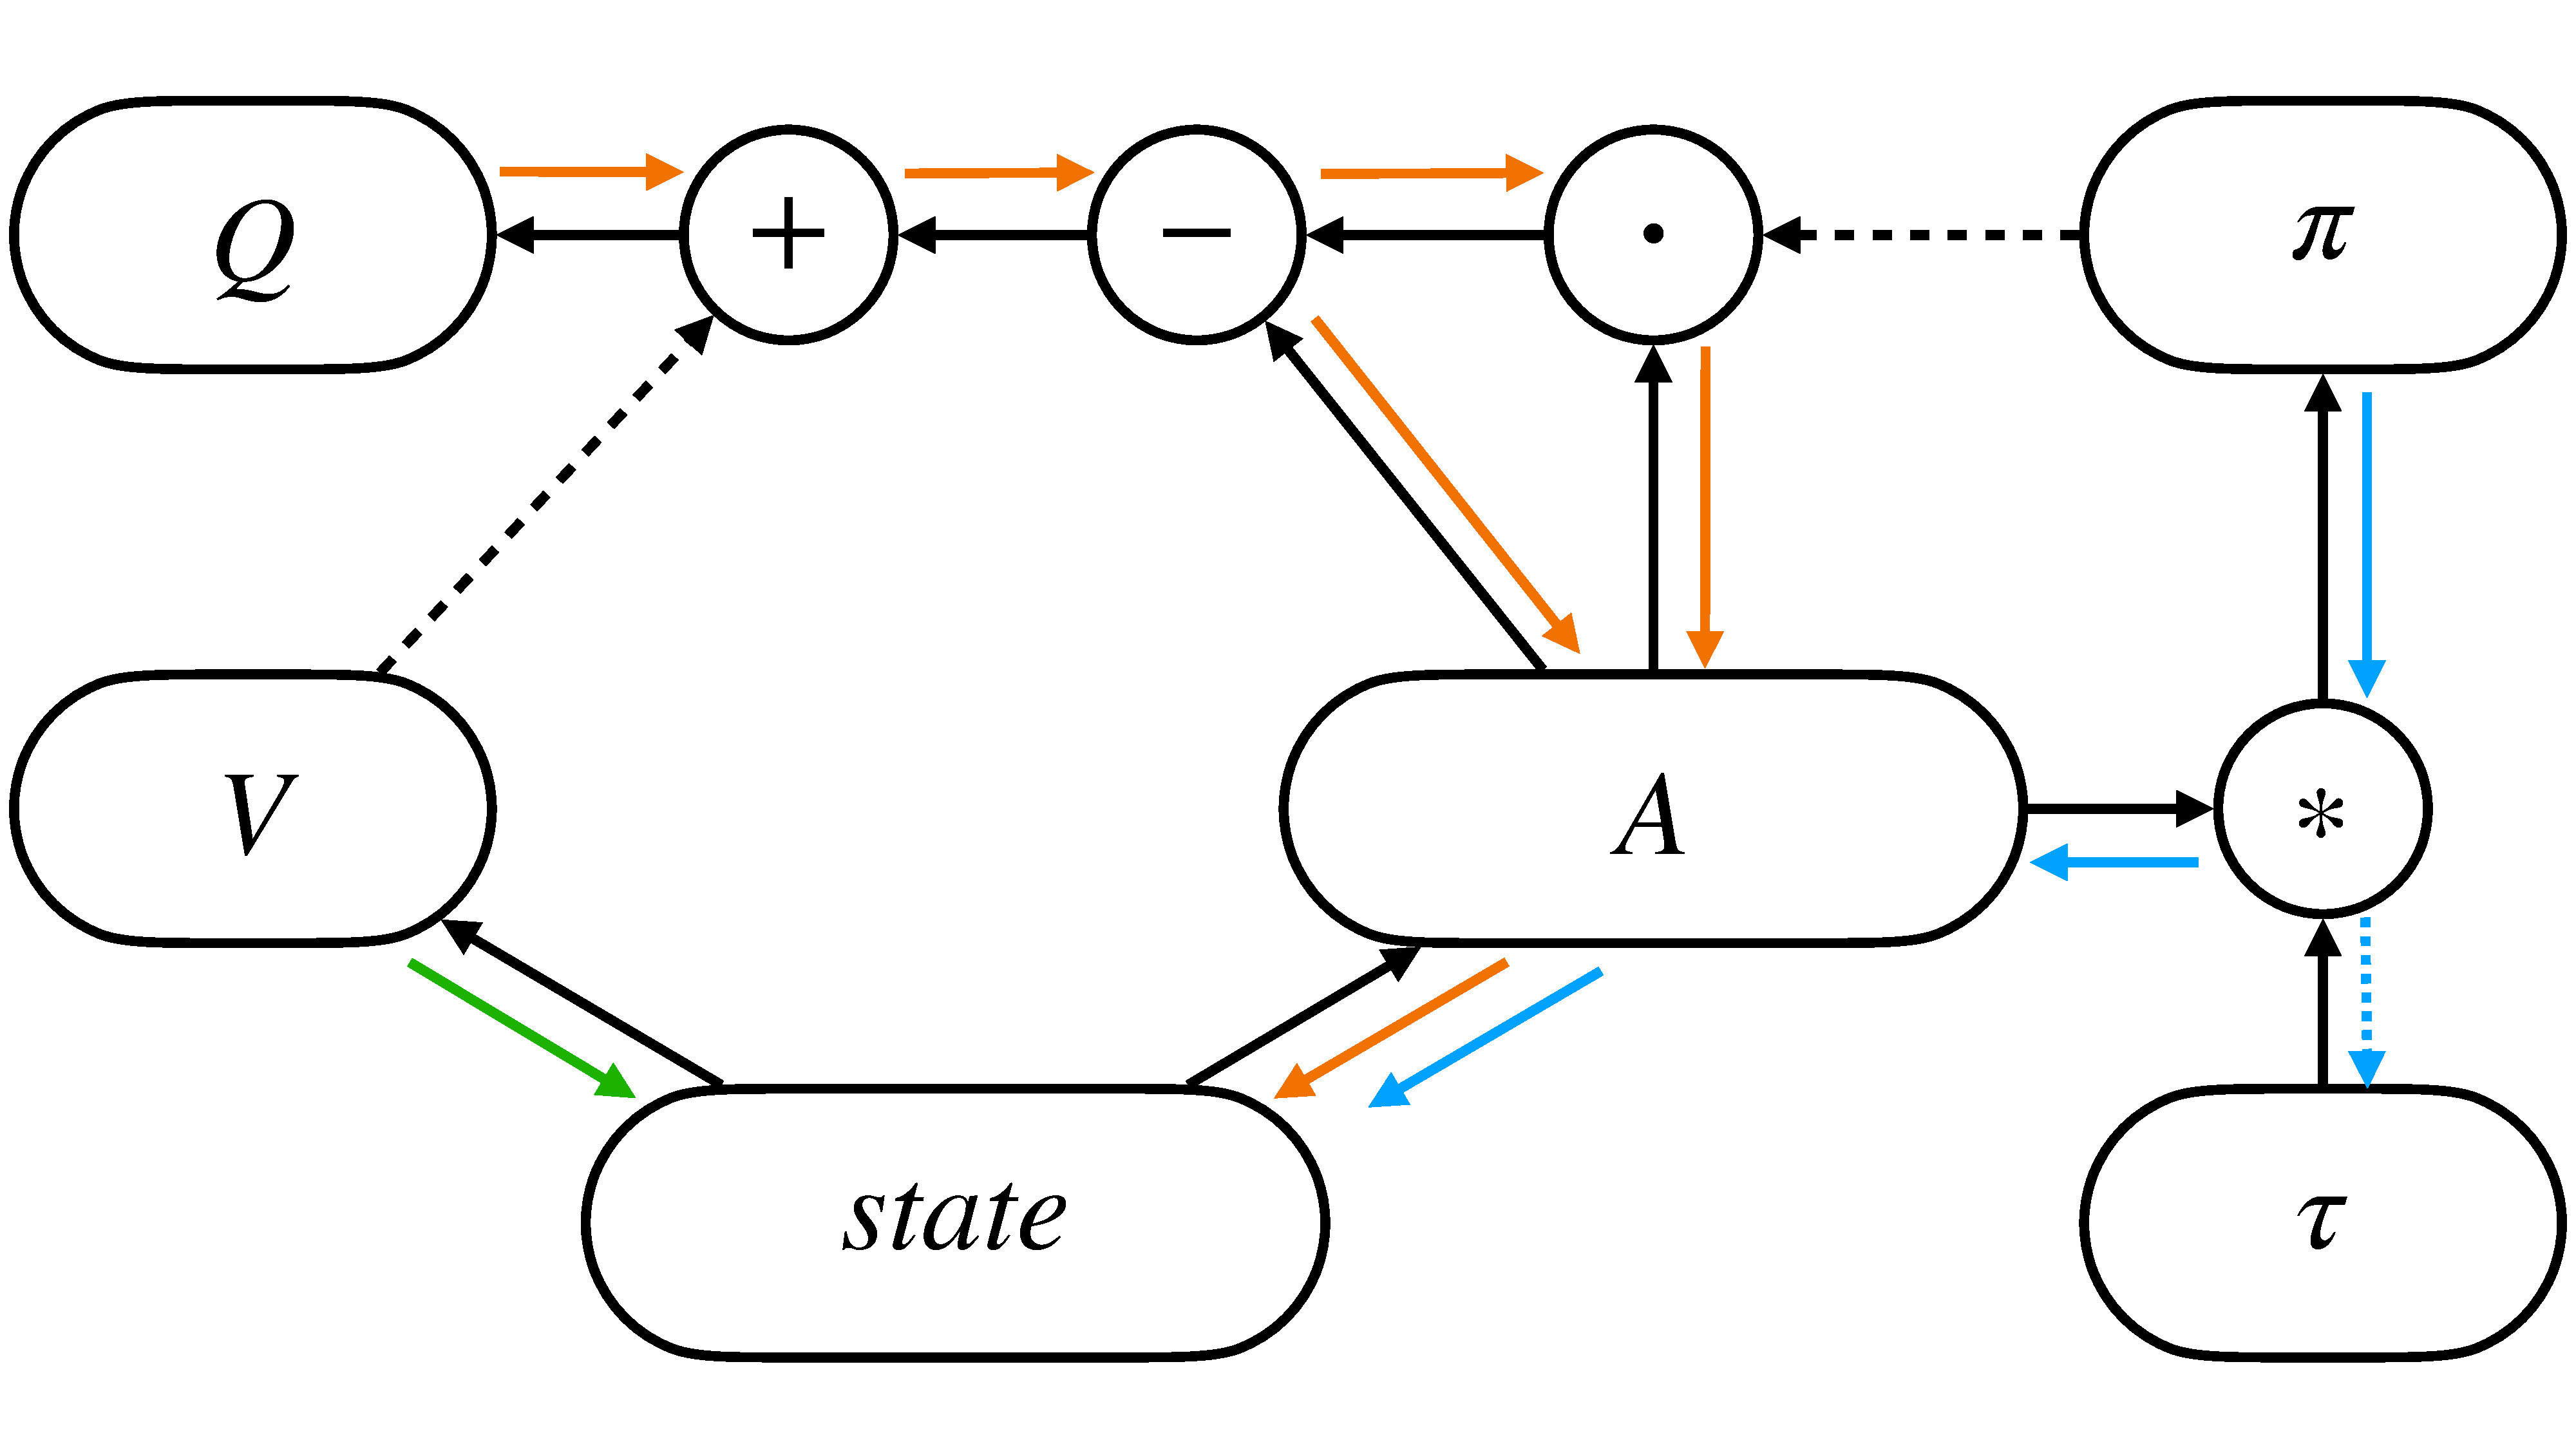
\includegraphics[width=0.4\textwidth,bb= 0 0 1800 1100]{body/figures/CASA.pdf}
% \caption{
% \textbf{Black} lines represent the forward process.
% \textbf{Dotted} black lines represent the \textit{stop gradient} operator in the forward process. 
% \textbf{Colorful} lines represent backpropagation from different loss functions. 
% Specifically, \textbf{blue} lines represent $\mathbb{E}_\pi [(Q^\pi-V)\nabla \log \pi]$, 
% \textbf{orange} lines represent $\mathbb{E}_\pi [(Q^\pi-Q)\nabla Q]$,
% and \textbf{green} lines represent $\mathbb{E}_\pi [(Q^\pi-V)\nabla V]$.}
% \label{fig:casa}
% \end{figure}
% \section{motivation experiments}

\clearpage

{\colorred \section{On Discussing Application of CASA on Continuous Action Space}
\label{app:cts_space}

As we can see CASA is only applied to discrete action space in the main context, we make a discussion on whether CASA is applicable on continuous action space. 
For brevity, we let $\tau=1$ and write \eqref{eq:casa} as:
\begin{equation}
\left\{
    \begin{aligned}
        &\pi = \text{softmax}(A), \\
        &\Bar{A} = A - \mathbb{E}_{\pi} [A], \\
        &Q = \Bar{A} + sg(V).
    \end{aligned}
\right. 
\end{equation}
The difficulty comes from estimating two quantities, one is $\text{softmax}(A)$, the other is $\mathbb{E}_{\pi} [A]$. 
This comes from the fact that discrete action space is countable so these two quantities are expressed in a closed-form, while continuous action space is uncountable so an accurate estimation of these two quantities is intractable. 
We can surely apply Monte Carlo methods to approximate, but a more elegant close-form expression may be preferred. 
Then this becomes another problem: \textit{how to estimate (state-action values / advantages / policy probabilities) of all actions in a continuous action space efficiently without loss of generality?}
This is another representational design problem, which is out of scope of this paper, so we don't touch much about it. 
But with the hope of inspiring a better solution to this problem, we provide one practical way of applying CASA on continuous action space based on kernel-based machine learning. 

Let $a_0, \dots, a_k$ to be basis actions in the action space. 
Let $A(s, a_0), \dots, A(s, a_k)$ to be advantage functions for tuples of states and basis actions. 
They can either share parameters or be isolated. 
Let $K(\cdot, \cdot)$ be a kernel function defined on the product of two action spaces. 
For any $a$ in the action space, we can estimate $A(s, a)$ by a decomposition such like $$A(s, a) = \frac{1}{Z_a} (K(a_0, a) A(s, a_0) + \dots + K(a_k, a) A(s, a_k)),$$ where $Z_a = \sum_{i=0}^k K(a_i, a)$ is a normalization constant. 

Since $K(\cdot, a)$ is a closed-form function of $a$, and $|\{A(s, a_0), \dots, A(s, a_k)\}|$ is finite, we can make a closed-form expression of both $\text{softmax}(A)$ and $\mathbb{E}_{\pi} [A]$. 
Then we can apply CASA directly on this expression, with one function estimates $V$ and the other function estimates advantages of all actions in a closed-form with only state as input.  
The policy is defined directly by $\text{softmax}$ of all advantages. 
In details, we define
\begin{equation}
\left\{
    \begin{aligned}
        &\pi(s, a) = \exp (A(s, a)) / \int_{a} \exp (A(s, a)) da, \\
        &\Bar{A}(s, a) = A(s, a) - \int_{a} sg(\pi(s, a)) A(s, a) da, \\
        &Q(s, a) = \Bar{A}(s, a) + sg(V(s)).
    \end{aligned}
\right. 
\end{equation}

Then it satisfies the consistency of CASA on continuous action space.
$$
\begin{aligned}
    \nabla \log \pi(s, a) &= \nabla A(s, a) - \frac{\nabla \int_{a} \exp (A(s, a)) da}{\int_{a} \exp (A(s, a)) da} \\
    &= \nabla A(s, a) - \frac{ \int_{a} \exp (A(s, a)) \nabla A(s, a) da}{\int_{a} \exp (A(s, a)) da} \\
    &= \nabla A(s, a) - \int_{a} \frac{  \exp (A(s, a)) }{\int_{a} \exp (A(s, a)) da} \nabla A(s, a) da \\
    &= \nabla A(s, a) - \int_{a} \pi(s, a) \nabla A(s, a) da \\
    &= \nabla \Bar{A}(s, a) = \nabla Q(s, a). 
\end{aligned}
$$
}

\section{DR-Trace}
\label{app:drtrace}

% One simple choice is to learn $V$ and $\pi$ by V-Trace \citep{impala} and to learn $Q$ by ReTrace \citep{retrace}. 
% \citep{impala} shows that $V^{\Tilde{\pi}}$ estimated by V-Trace converges to $V^*$ that corresponds to some $\Tilde{\pi}_{VTrace}$.
% Respectively, \citep{retrace} shows that $Q^{\Tilde{\pi}}$ estimated by ReTrace converges to $Q^*$ that corresponds to some $\Tilde{\pi}_{ReTrace}$.

As CASA estimates $(V, Q, \pi)$, we would ask
\textbf{i)} how to guarantee that $\Tilde{\pi}_{VTrace} = \Tilde{\pi}_{ReTrace}$, 
\textbf{ii)} how to exploit $(V, Q, \pi)$ to make a better estimation. 
Though we can apply V-Trace to estimate $V$ and ReTrace to estimate $Q$ with proper hyperparameters to guarantee $\Tilde{\pi}_{VTrace} = \Tilde{\pi}_{ReTrace}$, it's more reasonable to estimate $(V, Q)$ together. 
Inspired by Doubly Robust, which is shown to maximally reduce the variance, we introduce DR-Trace, which estimates $V$ by 
$$
\label{eq:dr-v}
    \begin{aligned}
        V_{DR}^{\Tilde{\pi}} (s_t) &\overset{def}{=} \mathbb{E}_{\mu} [ 
        V(s_t) + \sum_{k \geq 0} \gamma^k 
     c_{[t:t+k-1]} \rho_{t+k}  \delta^{DR}_{t+k} ],  
    \end{aligned}
$$
{\colorred where $\mu$ is the behavior policy}, $\delta^{DR}_t \overset{def}{=} r_t + \gamma V(s_{t+1}) - Q(s_t, a_t)$ is one-step Doubly Robust error, $\rho_t \overset{def}{=} \min\{\frac{\pi_t}{\mu_t}, \Bar{\rho} \}$ and $c_t \overset{def}{=} \min\{\frac{\pi_t}{\mu_t}, \Bar{c}\}$ are clipped per-step importance sampling, $c_{[t: t+k]} \overset{def}{=} \prod_{i=0}^{k} c_{t+i}$.

With one step Bellman equation, we estimate $Q$ by
$$
\label{eq:dr-q}
    \begin{aligned}
         Q_{DR}^{\Tilde{\pi}} (s_t, a_t) 
         &\overset{def}{=} \mathbb{E}_{s_{t+1}, r_t \sim p(\cdot, \cdot | s_t, a_t)} [  r_t + \gamma   V_{DR}^{\Tilde{\pi}} (s_{t+1}) ] 
        \\
        %  &=  \mathbb{E}_{\mu} [ r_t + \gamma V(s_{t + 1}) +
        % \gamma \sum_{k \geq 0} \gamma^k 
        % c_{[t+1:t+k]} \rho_{t+1+k}
        % \delta^{DR}_{t+1+k} V
        % ]
        % \\
        %  &= \mathbb{E}_{\mu}   [
        % Q(s_t, a_t) + \delta_t^{DR}V + \sum_{k \geq 1}  \gamma^k
        % c_{[t+1:t+k-1]} \rho_{t+k}
        % \delta^{DR}_{t+k} V
        % ],
        % \\
        &=  \mathbb{E}_{\mu}   [
        Q(s_t, a_t) + \sum_{k \geq 0}  \gamma^k
        c_{[t+1:t+k-1]} \Tilde{\rho}_{t, k}
        \delta^{DR}_{t+k}
        ], 
    \end{aligned}
$$
where $\Tilde{\rho}_{t, k} =  1_{\{k=0\}} + 1_{\{k > 0\}} \rho_{t+k}$.

% Compared to \eqref{eq:dr-v}, $c_{[t+1:t+k-1]} \Tilde{\rho}_{t, k}$ in \eqref{eq:dr-q} doesn't multiply importance sampling ratio of $a_t$, which meets the same intuition as \eqref{eq:vtrace} and \eqref{eq:retrace}.\\
\begin{theorem}
    Define $\Bar{A} = A - \mathbb{E}_\pi[A]$, $Q = \Bar{A} + sg(V)$,
    $$
    \begin{aligned}
    &\mathscr{T}(Q) \overset{def}{=} \mathbb{E}_{\mu}   [
        Q(s_t, a_t) + \sum_{k \geq 0}  \gamma^k
        c_{[t+1:t+k-1]} \Tilde{\rho}_{t, k}
        \delta^{DR}_{t+k}
        ], \\
    &\mathscr{S}(V) \overset{def}{=} \mathbb{E}_{\mu}   [
        V(s_t) + \sum_{k \geq 0}  \gamma^k
        c_{[t:t+k-1]} \rho_{t, k}
        \delta^{DR}_{t+k}
        ], \\
    &\mathscr{U}(Q, V) = (\mathscr{T}(Q) - \mathbb{E}_\pi[Q] + \mathscr{S}(V), \mathscr{S}(V)), \\
    &\mathscr{U}^{(n)}(Q, V) = \mathscr{U}(\mathscr{U}^{(n-1)}(Q, V)),
    \end{aligned}
    $$
    then $\mathscr{U}^{(n)}(Q, V) \rightarrow (Q^{\Tilde{\pi}}, V^{\Tilde{\pi}})$ that corresponds to 
    $$
        \Tilde{\pi}(a|s) = \frac
        {\min \left\{\Bar{\rho} \mu (a|s), \pi(a|s)\right\}}
        {\sum_{b \in \mathcal{A}}\min \left\{\Bar{\rho} \mu (b|s), \pi(b|s)\right\}}.
    $$ as $n \rightarrow +\infty$.
\label{thm:dr}
\end{theorem}
\begin{proof}
    See Appendix \ref{app:proof}, Theorem \ref{thm_app:dr}.
\end{proof}
Theorem \ref{thm:dr} shows that DR-Trace is a contraction mapping and $(V, Q)$ converges to $(V^{\Tilde{\pi}}, Q^{\Tilde{\pi}})$ that corresponds to 
$$
    \begin{aligned}
        \Tilde{\pi}(a|s) = \frac
        {\min \left\{\Bar{\rho} \mu (a|s), \pi(a|s)\right\}}
        {\sum_{b \in \mathcal{A}}\min \left\{\Bar{\rho} \mu (b|s), \pi(b|s)\right\}}.
    \end{aligned}
$$

% At training time, the policy evaluation is achieved by updating $\theta$ to minimize $l2$ losses
% $$
% \begin{aligned}
%     L_V(\theta) &= \mathbb{E}_\pi [ (V_\theta(s_t) -  V_{DR}^{\Tilde{\pi}} (s_t))^2 ], \\
%     L_Q(\theta) &= \mathbb{E}_\pi [ (Q_\theta(s_t, a_t) -  Q_{DR}^{\Tilde{\pi}} (s_t, a_t))^2 ],
% \end{aligned}
% $$ 
% which gives the ascent direction of $\theta$ by
% \begin{equation}
% \label{eq:grad_qv}
%     \begin{aligned}
%         \nabla_\theta L_V(\theta)
%         &= \mathbb{E}_\pi \left[ (V_{DR}^{\Tilde{\pi}} (s_t) - V_\theta(s_t) ) \nabla V_\theta(s_t) \right], \\
%         \nabla_\theta L_Q(\theta)
%         &= \mathbb{E}_\pi \left[ (Q_{DR}^{\Tilde{\pi}} (s_t, a_t) - Q_\theta(s_t, a_t)) \nabla Q_\theta(s_t, a_t) \right].
%     \end{aligned}
% \end{equation}
% And we make the policy improvement by policy gradient, which gives the ascent direction of $\theta$ by 
% \begin{equation}
% \label{eq:grad_pi}
% \begin{aligned}
%     \nabla_\theta \mathcal{J}(\tau, \theta) = \mathbb{E}_\mu \left[\tau \rho_t (Q_{DR}^{\Tilde{\pi}} (s_t, a_t) - V_\theta(s_t) ) \nabla_\theta \log \pi_t \right],
% \end{aligned}
% \end{equation}
% where $\mathcal{J} (\tau, \theta) = \tau \mathbb{E}_\pi [\sum \gamma^t r_t]$.
% It takes an additional $\tau$, which frees the scale of gradient from $\tau$.

% Finally, the gradient ascent direction of $\theta$ is given by
% \begin{equation}
%     \label{eq:grad_all}
%     \alpha_1 \nabla_\theta L_V + \alpha_2 \nabla_\theta L_Q + \alpha_3 \nabla_\theta \mathcal{J}.
% \end{equation}

% \textbf{Full algorithm is described in Appendix \ref{app:casa}.}
% Note that \eqref{eq:grad_all} doesn't need any entropy regularization. 
% We will discuss why this happens in section \ref{sec:equiv} and how CASA controls the exploration in section \ref{sec:ent_control}.


\begin{figure}[h]
    \centering
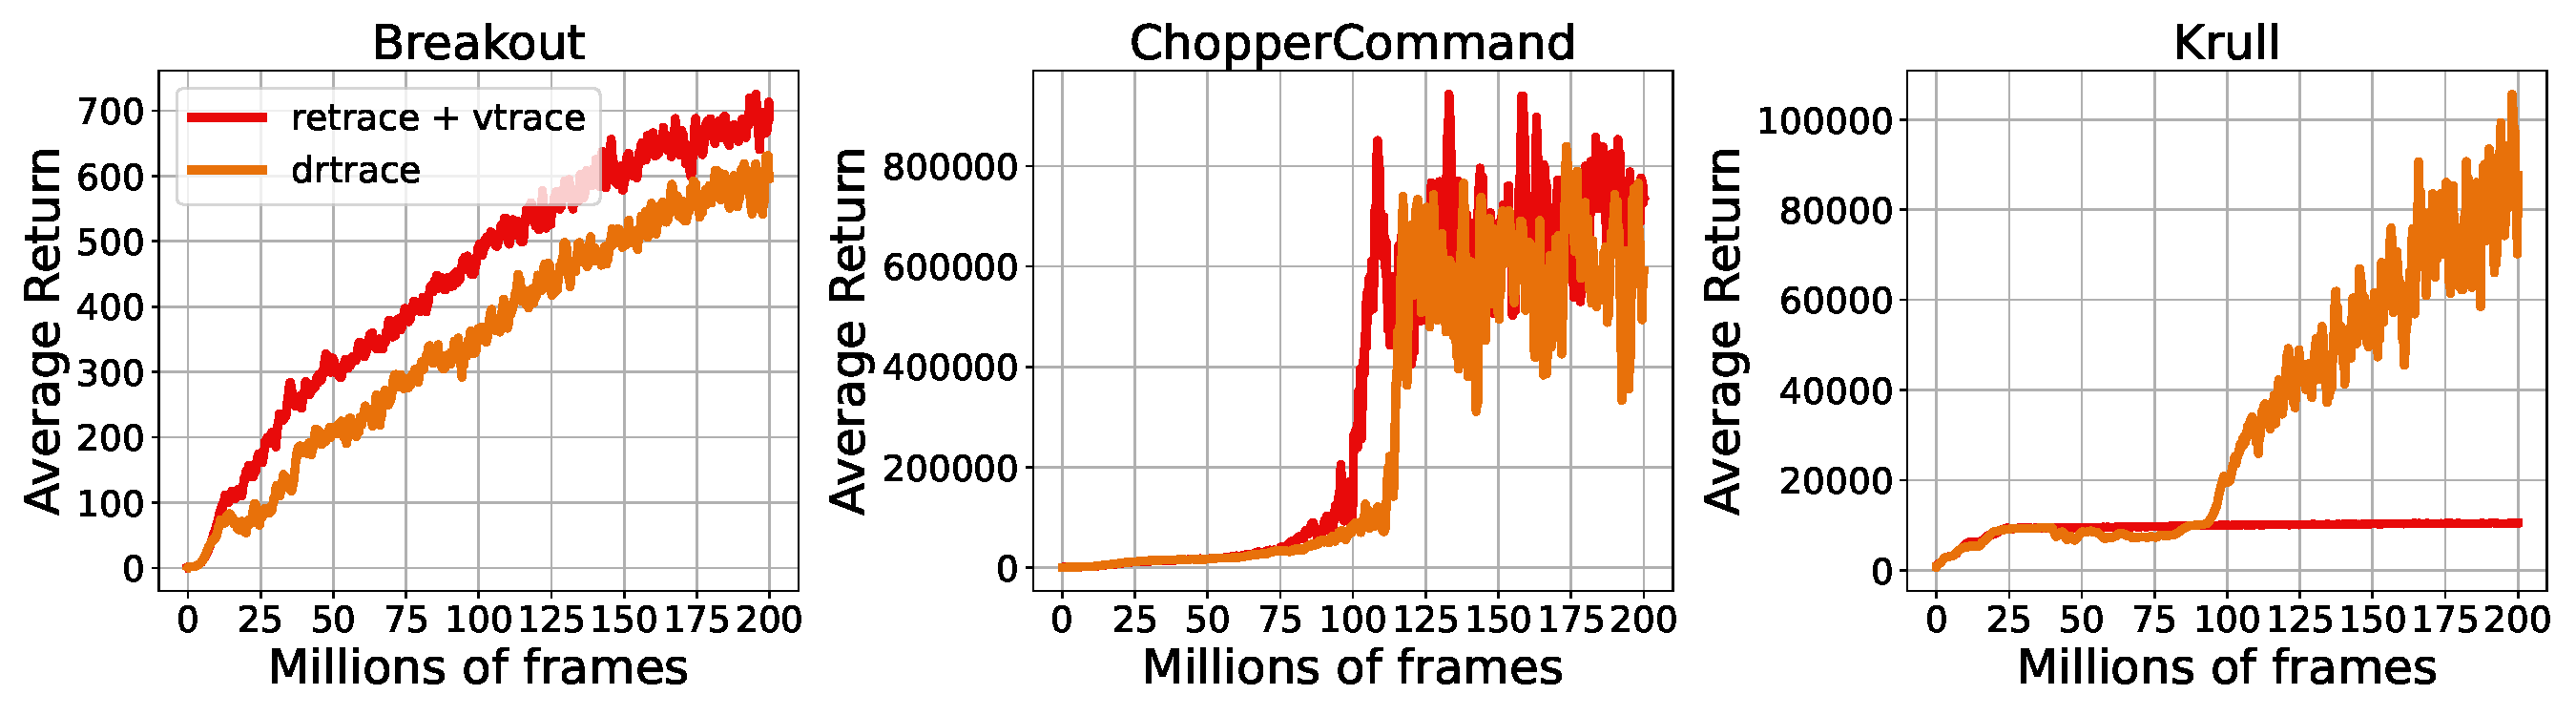
\includegraphics[width=\linewidth]{body/ablation/dr_ablation.pdf}
    \caption{Ablation study for w/wo DR-Trace on Breakout, ChopperCommand and Krull.}
    \label{fig:app_dr_trace}
\end{figure}

According to our proof, DR-Trace should work similar to V-Trace and ReTrace, as the convergence rate and the limitation are same. 
We compare DR-Trace with V-Trace+ReTrace in Figure \ref{fig:app_dr_trace}, where we replace estimation of state values by V-Trace and estimation of state-action values by ReTrace. 
We call V-Trace+ReTrace as No-DR-Trace for brevity. 
No-DR-Trace performs better on Breakout and ChopperCommand, but fails to make a breakthrough on Krull. 
Recalling the fact that Doubly Robust can maximally reduce the variance of Bellman error, No-DR-Trace is less stable but also potential to achieve a better performance. 
A conclusion cannot be made about No-DR-Trace, as this phenomenon means that No-DR-Trace is less stable than DR-Trace, but it also holds the potential to achieve a better performance.

% \clearpage


\section{Proofs}
\label{app:proof}

\theoremstyle{plain}
% \setcounter{Lemma}{0}
\newtheorem{Lemma_app}{Lemma}[section]
\newtheorem{Theorem_app}{Theorem}[section]
\theoremstyle{definition}
\newtheorem*{Remark_app}{Remark}
\theoremstyle{remark}

% \begin{Lemma_app}
% Let 
% $g \in \textbf{C}^{1}(\mathbb{R}^{n}): \mathbb{R}^{n} \to \mathbb{R}^{n}, \ f \in \textbf{C}^{1}(\mathbb{R}^{n+k}): \mathbb{R}^{n+k} \to \mathbb{R}^{n}.
% $\\
% If
% $
% \nabla_x g(x) = \nabla_x f(x, y)$, for $\forall x\in \mathbb{R}^{n}, y\in \mathbb{R}^k,
% $
% then $\exists$ $c \in \textbf{C}^{1}(\mathbb{R}^{k}): \mathbb{R}^{k} \to \mathbb{R}^{n}$, s.t. $f(x, y) = g(x) + c(y)$.
% \label{lemma_app:func_sep}
% \end{Lemma_app}
% \begin{proof}

% Let $\Tilde{f}(x, y) = f(x, y) - g(x)$.

% Since $\nabla_x g(x) = \nabla_x f(x, y)$, we have 
% $$
% \nabla_x \Tilde{f} = 0, \ for \ \forall x\in \mathbb{R}^{n}, y\in \mathbb{R}^k.
% $$

% So $\Tilde{f}$ is a constant function w.r.t $x$, which can be denoted as $c(y) = \Tilde{f}(x, y)$.

% Hence, $f(x, y) = g(x) + c(y)$.
% \end{proof}

\begin{Lemma_app}
(i) Define $\pi = softmax(A / \tau)$, then $\nabla \log \pi = (\textbf{1} - \pi) \frac{\nabla A}{\tau}$. 
(ii) Denote $sg$ to be stop gradient and define $\Bar{A} = A - \mathbb{E}_\pi [A]$, $Q = \Bar{A} + sg(V)$, then $\nabla Q = (\textbf{1} - \pi) \nabla A$.
\label{lemma_app:vannila_grad}
\end{Lemma_app}
\begin{proof}

As $Q = \Bar{A} + sg(V) = A - sg(\pi)\cdot A + sg(V)$, it's obvious that $\nabla Q = (\textbf{1} - \pi) \nabla A$.

For $\log \pi$, it's a standard derivative of cross entropy, so we have $\nabla \log \pi = (\textbf{1} - \pi) \nabla (A / \tau) = (\textbf{1} - \pi) \frac{\nabla A}{\tau}$.
\end{proof}

\begin{Lemma_app}
Define $\Bar{A}= A - \mathbb{E}_\pi[A]$, $Q = \Bar{A} + sg(V), \pi = softmax(A / \tau)$, then 
$$
\mathbb{E}_\pi \left[ (Q - V) \nabla \log \pi \right]
= - \tau \nabla \textbf{H}[\pi].
$$
\label{lemma_app:eqiv_pg_ent}
\end{Lemma_app}
\begin{proof}
Since 
$$
\pi = \exp(A / \tau) / Z,\ Z = \int_\mathcal{A} \exp(A / \tau),
$$
we have 
$$
A = \tau \log \pi + \tau \log Z.
$$
Based on the observation that $\mathbb{E}_\pi \left[ f(s) \nabla \log \pi (\cdot | s) \right] = 0$, 
we have 
$$\mathbb{E}_\pi \left[ \mathbb{E}_\pi[A] \cdot \nabla \log \pi \right] = 0,$$ 
$$\mathbb{E}_\pi \left[ \log Z \cdot \nabla \log \pi \right] = 0.$$

On the one hand,
$$
\begin{aligned}
    \mathbb{E}_\pi \left[ (Q - V) \nabla \log \pi \right]
    &= \mathbb{E}_\pi \left[ A \nabla \log \pi \right] 
    - \mathbb{E}_\pi \left[ \mathbb{E}_\pi[A] \cdot \nabla \log \pi \right] \\
    &= \tau \mathbb{E}_\pi \left[ \log \pi \nabla \log \pi \right]
    + \tau \mathbb{E}_\pi \left[ \log Z \cdot \nabla \log \pi \right] \\
    &= \tau \mathbb{E}_\pi \left[ \log \pi \nabla \log \pi \right].
\end{aligned}
$$

On the other hand, 
$$
\begin{aligned}
    \nabla \textbf{H} [\pi] 
    &= - \nabla \int_\mathcal{A} \pi_i \log \pi_i \\
    &= - \int_\mathcal{A}  \nabla \pi_i \cdot \log \pi_i - \int_\mathcal{A} \pi_i \nabla \log \pi_i  \\
    &= - \int_\mathcal{A}  \pi_i \nabla \log \pi_i \cdot \log \pi_i - \int_\mathcal{A}  \pi_i \frac{\nabla \pi_i}{\pi_i} \\
    &= - \mathbb{E}_\pi \left[ \log \pi \nabla \log \pi \right].
\end{aligned}
$$
Hence, $
\mathbb{E}_\pi \left[ (Q - V) \nabla \log \pi \right]
= - \tau \nabla \textbf{H}[\pi]
$.
\end{proof}

\begin{Theorem_app}
    Define $\Bar{A} = A - \mathbb{E}_\pi[A]$, $Q = \Bar{A} + sg(V)$.
    Define $$
    \begin{aligned}
    &\mathscr{T}(Q) \overset{def}{=} \mathbb{E}_{\mu}   [
        Q(s_t, a_t) + \sum_{k \geq 0}  \gamma^k
        c_{[t+1:t+k-1]} \Tilde{\rho}_{t, k}
        \delta^{DR}_{t+k}
        ], \\
    &\mathscr{S}(V) \overset{def}{=} \mathbb{E}_{\mu}   [
        V(s_t) + \sum_{k \geq 0}  \gamma^k
        c_{[t:t+k-1]} \rho_{t, k}
        \delta^{DR}_{t+k}
        ], \\
    &\mathscr{U}(Q, V) = (\mathscr{T}(Q) - \mathbb{E}_\pi[Q] + \mathscr{S}(V), \mathscr{S}(V)), \\
    &\mathscr{U}^{(n)}(Q, V) = \mathscr{U}(\mathscr{U}^{(n-1)}(Q, V)),
    \end{aligned}
    $$
    then $\mathscr{U}^{(n)}(Q, V) \rightarrow (Q^{\Tilde{\pi}}, V^{\Tilde{\pi}})$ that corresponds to 
    $$
        \Tilde{\pi}(a|s) = \frac
        {\min \left\{\Bar{\rho} \mu (a|s), \pi(a|s)\right\}}
        {\sum_{b \in \mathcal{A}}\min \left\{\Bar{\rho} \mu (b|s), \pi(b|s)\right\}}.
    $$ as $n \rightarrow +\infty$.
\label{thm_app:dr}
\end{Theorem_app}
\begin{Remark_app}
$\mathscr{T}(Q) - \mathbb{E}_\pi[Q] + \mathscr{S}(V)$ is \textbf{exactly} how $Q$ is updated at training time. 
Since $Q = \Bar{A} + sg(V)$, if we apply gradient ascent on $Q$ and $V$ in directions $\nabla L_Q(\theta)$ and $\nabla L_V(\theta)$ respectively, change of $Q$ comes from two aspects. One comes from $\nabla L_Q(\theta)$, which changes $A$, the other comes from $\nabla L_V(\theta)$, which changes $V$. Because the gradient of $V$ is stopped when estimating $Q$, the latter is captured by "minus old baseline, add new baseline", which is $- \mathbb{E}_\pi[Q] + \mathscr{S}(V)$ in Theorem \ref{thm_app:dr}.
\end{Remark_app}
\begin{proof}
 Define
 $$
 \begin{aligned}
        \widetilde{\mathscr{T}}(Q) &= - \mathbb{E}_\pi[Q] + \mathscr{T}(Q), \\
        \widetilde{\mathscr{U}}(Q, V) &= (\widetilde{\mathscr{T}}(Q), \mathscr{S}(V)), \\
        \widetilde{\mathscr{U}}^{(n)}(Q, V) &=   \widetilde{\mathscr{U}}(\widetilde{\mathscr{U}}^{(n-1)}(Q, V)).
 \end{aligned}
 $$
By Lemma \ref{lemma_app:dr_q}, $\widetilde{\mathscr{T}}^{(n)}(Q)$ converges to some $A^*$ as $n \rightarrow \infty$. This process will not influence the estimation of $V$ as the gradient of $V$ is stopped when estimating $Q$. According to the proof, $A^*$ does not depend on $V$. \\
By Lemma \ref{lemma_app:dr_v}, $\mathscr{S}^{(n)}(V)$ converges to some $V^*$ as $n \rightarrow \infty$. \\
Hence, we have
$$
\widetilde{\mathscr{U}}^{(n)}(Q, V) \rightarrow (A^*, V^*)\ \ as\ \ n \rightarrow +\infty. 
$$
By definition, 
$$
\mathscr{U}(Q, V) = (\widetilde{\mathscr{T}}(Q) + \mathscr{S}(V), \mathscr{S}(V)),
$$
we can regard $\widetilde{\mathscr{T}}(Q) + \mathscr{S}(V)$ as $Q$ and regard $\mathscr{S}(V)$ as $V$, then
$$
\begin{aligned}
    \mathscr{U}^{(2)}(Q, V) 
    &= \mathscr{U}(\widetilde{\mathscr{T}}(Q) + \mathscr{S}(V), \mathscr{S}(V)) \\
    &= (\mathscr{T}(\widetilde{\mathscr{T}}(Q) + \mathscr{S}(V)) -\mathscr{S}(V) + \mathscr{S}^{(2)}(V), \mathscr{S}^{(2)}(V)) \\
    &= (\widetilde{\mathscr{T}}^{(2)}(Q) + \mathscr{S}^{(2)}(V), \mathscr{S}^{(2)}(V)).
\end{aligned}
$$
By induction, 
$$
\begin{aligned}
    \mathscr{U}^{(n)}(Q, V) &= (\widetilde{\mathscr{T}}^{(n)}(Q) + \mathscr{S}^{(n)}(V), \mathscr{S}^{(n)}(V)) \\
    &\rightarrow (A^*+V^*, V^*)\ \ as\ \ n\rightarrow + \infty.
\end{aligned}
$$
Same as \citep{impala}, 
$$
    \Tilde{\pi}(a|s) = \frac
    {\min \left\{\Bar{\rho} \mu (a|s), \pi(a|s)\right\}}
    {\sum_{b \in \mathcal{A}}\min \left\{\Bar{\rho} \mu (b|s), \pi(b|s)\right\}}.
$$ 
is the policy s.t. the Bellman equation holds, which is 
$$\mathbb{E}_\mu[\rho_t (r_t + \gamma V_{t+1} - V_t) | \mathscr{F}_t] = 0,$$ and $\mathscr{U}(Q^{\Tilde{\pi}}, V^{\Tilde{\pi}}) = (Q^{\Tilde{\pi}}, V^{\Tilde{\pi}})$. \\
So we have
$(A^*+V^*, V^*) = (Q^{\Tilde{\pi}}, V^{\Tilde{\pi}}).$
\end{proof}

\begin{Lemma_app}
Define $\Bar{A}= A - \mathbb{E}_\pi[A]$, $Q = \Bar{A} + sg(V)$,
then operator 
$$
    \mathscr{T}(Q) \overset{def}{=} \mathbb{E}_{\mu}   [
        Q(s_t, a_t) + \sum_{k \geq 0}  \gamma^k
        c_{[t+1:t+k-1]} \Tilde{\rho}_{t, k}
        \delta^{DR}_{t+k}
        ]
$$
is a contraction mapping w.r.t. $Q$.
\label{lemma_app:dr_q}
\end{Lemma_app}
\begin{Remark_app}
Note that $\mathscr{T}(Q)$ is exactly \eqref{eq:dr-q}. 

Since $Q = A + sg(V)$, the gradient of $V$ is stopped when estimating $Q$, updating $Q$ will not change $V$, which is equivalent to updating $A$.
Without loss of generality, we assume $V$ is fixed as $V^*$ in the proof.
\end{Remark_app}
\begin{proof}

$\Bar{A} = A - \mathbb{E}_\pi[A]$ shows $\mathbb{E}_\pi[\Bar{A}] = 0$, which guarantees that no matter how we update $A$, we always have $\mathbb{E}_\pi[Q] = V^*$.

Based on above observations, define 
$$
    \widetilde{\mathscr{T}}(Q) \overset{def}{=} - \mathbb{E}_\pi [Q] + \mathscr{T}(Q).
$$

It's obvious that we only need to prove $\widetilde{\mathscr{T}}(Q)$ is a contraction mapping.

For brevity, we denote $$Q_t = Q(s_t, a_t), A_t = A(s_t, a_t), V^*_t = V^*(s_t).$$

Noticing that $\Tilde{\rho}_{t, 0} = 1$, let $\mathscr{F}$ represent filtration, we can rewrite $\widetilde{\mathscr{T}}$ as 
\begin{equation}
\label{eq:dr_a_2}
\begin{aligned}
    \widetilde{\mathscr{T}}(Q)
    &= \mathbb{E}_{\mu}   [
        A_t + \sum_{k \geq 0}  \gamma^k
        c_{[t+1:t+k-1]} \Tilde{\rho}_{t, k}
        \delta^{DR}_{t+k}
        ] \\
    &= \mathbb{E}_{\mu}   [
        -V^*_t + \sum_{k \geq 0}  \gamma^k
        c_{[t+1:t+k-1]} \Tilde{\rho}_{t, k}
        r_{t+k}
        + 
        \sum_{k \geq 0}  \gamma^{k+1}
        c_{[t+1:t+k-1]} \Delta_k ],
        \\
\end{aligned}
\end{equation}
where 
\begin{equation}
\label{eq:dr_delta}
    \Delta_k = \mathbb{E}_{\mu}\left[\Tilde{\rho}_{t, k} V^*_{t+k+1} - c_{t+k} \Tilde{\rho}_{t, k+1} Q_{t+k+1} | \mathscr{F}_{t+k}\right].
\end{equation}
By definition of $Q$,
$$
    \mathbb{E}_{\mu}[V_{t+k+1}^*|\mathscr{F}_{t+k}] 
    = \mathbb{E}_{\mu}[
    \mathbb{E}_\pi[Q_{t+k+1}|\mathscr{F}_{t+k+1}]
    |\mathscr{F}_{t+k}], \\
    % \geq&  \mathbb{E}_{\mu}[
    % \mathbb{E}_\mu[\Tilde{\rho}_{t, k+1} Q_{t+k+1}|\mathscr{F}_{t+k+1}]
    % |\mathscr{F}_{t+k}], 
$$
we can rewrite \eqref{eq:dr_delta} as
\begin{equation}
\label{eq:dr_q_delta}
\Delta_k = \mathbb{E}_{\mu}[
(
\Tilde{\rho}_{t, k} \frac{\pi_{t+k+1}}{\mu_{t+k+1}}- c_{t+k} \Tilde{\rho}_{t, k+1} 
) Q_{t+k+1} | \mathscr{F}_{t+k}
].
\end{equation}
For any $Q_1 = A_1 + sg(V^*)$, $Q_2 = A_2 + sg(V^*)$, since
$$
\mathbb{E}_{\mu}[
(
\Tilde{\rho}_{t, k} \frac{\pi_{t+k+1}}{\mu_{t+k+1}}- c_{t+k} \Tilde{\rho}_{t, k+1} 
) | \mathscr{F}_{t+k}
] \geq 0,
$$
by \eqref{eq:dr_a_2} \eqref{eq:dr_q_delta}, we have 
% $$
% || \Delta^1_k - \Delta_k^2 || \leq \mathbb{E}_{\mu}\left[
% \left(
% \Tilde{\rho}_{t, k} \frac{\pi_{t+k+1}}{\mu_{t+k+1}}- c_{t+k} \Tilde{\rho}_{t, k+1} 
% \right) | \mathscr{F}_{t+k}
% \right] ||A^1 - A_2||.
% $$
$$
        || \widetilde{\mathscr{T}}(Q_1) - \widetilde{\mathscr{T}}(Q_2) || 
        % \leq& \mathbb{E}_{\mu} \left[ \sum_{k \geq 0}  \gamma^{k+1} c_{[t+1:t+k-1]} || \Delta_k^1 - \Delta_k^2 || \right] \\
        \leq \mathcal{C} || Q_1 - Q_2 ||,
$$
where 
$$
    \begin{aligned}
        \mathcal{C} 
        &= \mathbb{E}_{\mu} [ \sum_{k \geq 0}  \gamma^{k+1} c_{[t+1:t+k-1]} 
        (
        \Tilde{\rho}_{t, k} \frac{\pi_{t+k+1}}{\mu_{t+k+1}}- c_{t+k} \Tilde{\rho}_{t, k+1} 
        ) ]
        \\
        &= \mathbb{E}_{\mu} [1 -1 + \sum_{k \geq 0}  \gamma^{k+1} c_{[t+1:t+k-1]} 
        \left(
        \Tilde{\rho}_{t, k} - c_{t+k} \Tilde{\rho}_{t, k+1} 
        \right) ] 
        \\
        &= 1 - (1 - \gamma)  \mathbb{E}_{\mu} [\sum_{k \geq 0} \gamma^{k}c_{[t+1:t+k-1]} \Tilde{\rho}_{t, k}  ] \\
        &\leq 1 - (1 - \gamma) < 1.
    \end{aligned}
$$
Hence, $\widetilde{\mathscr{T}}(Q)$ is a contraction mapping and converges to some fixed function, which we denote as $A^*$. So $\mathscr{T}(Q)$ is also a contraction mapping and converges to $A^*+V^*$.
\end{proof}

\begin{Lemma_app}
Define $Q = A + sg(V)$ with $\mathbb{E}_\pi [A] = 0$,
then operator 
$$
    \mathscr{S}(V) \overset{def}{=} \mathbb{E}_{\mu}  [
        V(s_t) + \sum_{k \geq 0}  \gamma^k
        c_{[t:t+k-1]} \rho_{t, k}
        \delta^{DR}_{t+k}
        ]
$$
is a contraction mapping w.r.t. $V$.
\label{lemma_app:dr_v}
\end{Lemma_app}
\begin{Remark_app}
Note that $\mathscr{S}(V)$ is exactly \eqref{eq:dr-v}. 
\end{Remark_app}
\begin{proof}

% Since $Q = A + sg(V)$, updating $V$ wouldn't influence $A$. WLOG, we assume $A$ is fixed as $A^*$ in Lemma \ref{lemma_app:dr_v}. \\
Same as Lemma \ref{lemma_app:dr_q}, we can get
$$
    \Delta_k = \mathbb{E}_{\mu}\left[
    \left( \rho_{t+k} - c_{t+k} \rho_{t+k+1}\right) V_{t+k+1} 
     -  c_{t+k} \rho_{t+k+1} A^*_{t+k+1} | \mathscr{F}_{t+k}\right],
$$
so we have 
$$
    \Delta^1_k - \Delta^2_k = \mathbb{E}_{\mu}\left[ 
    \left( \rho_{t+k} - c_{t+k} \rho_{t+k+1}\right) \cdot  
   (V^1_{t+k+1} -  V^2_{t+k+1})
     | \mathscr{F}_{t+k}\right].
$$
The remaining proof is identical to \citep{impala}'s.
\end{proof}

% \clearpage

% \begin{Lemma_app}
% Let $v \in \mathbb{R}^{|\mathcal{A}|}$ to be a vector. 
% Define 
% $
%     \pi (\tau) = \exp (v / \tau) / Z,\  Z = \int_\mathcal{A}  \exp(v / \tau).
% $
% Let $\Omega$ to be a probability measure supported on $[K, +\infty]$,
% then $f(\Omega) = \mathbb{E}_{\tau \sim \Omega} [\mathbb{E}_{\pi(\tau)} [v]]$ satisfies Lipschitz-1 condition with Wasserstein-1 metric.
% \label{lemma_app:lips}
% \end{Lemma_app}
% \begin{proof}
% Without loss of generality, we assume $v_1 \geq v_2 \geq ... \geq v_{|\mathcal{A}|}$.

% For any $\tau \in [0, +\infty)$, since
% $$
% \begin{aligned}
%     \pi (\tau) = \exp (v / \tau) / Z,\  Z = \int_\mathcal{A}  \exp(v / \tau),
% \end{aligned}
% $$
% we have
% $$
%     v = \tau \log \pi (\tau) + \tau \log Z.
% $$

% Denote $\Tilde{v}_j = v_j / \tau$. \\
% Since 
% $$
% \frac{\partial \log \pi_i}{\partial \Tilde{v}_j} = 1_{i=j} - \pi_j,
% $$
% we have
% $$
% \begin{aligned}
%     \frac{\partial \log \pi_i}{\partial \tau} 
%     &= \sum_j \frac{\partial \log \pi_i}{\partial \Tilde{v}_j} \cdot \frac{\partial \Tilde{v}_j}{\partial \tau} \\
%     &= - \sum_j (1_{i=j} - \pi_j) \frac{v_j}{\tau^2} \\
%     &= - \frac{1}{\tau^2} ( v_i - \sum_j \pi_j v_j ) \\ 
%     &= - \frac{1}{\tau^2} \left( v_i - \mathbb{E}_\pi [v] \right). 
% \end{aligned}
% $$
% Therefore, we have
% $$
% \begin{aligned}
%     \frac{\partial \pi_i}{\partial \tau} 
%     &= \pi_i \frac{\partial \log \pi_i}{\partial \tau} \\
%     &= - \frac{\pi_i}{\tau^2} \left( v_i - \mathbb{E}_\pi [v] \right).
% \end{aligned}
% $$
% Let $f(\tau) = v \cdot \pi(\tau)$, then
% $$
% \frac{\partial f}{\partial \tau} = - \frac{1}{\tau^2} \sum_i v_i \pi_i \left( v_i - \mathbb{E}_\pi [v] \right).
% $$
% Since $\sum_i \mathbb{E}_\pi [v] \pi_i \left( v_i - \mathbb{E}_\pi [v] \right) = 0$,
% we know
% $$
% \begin{aligned}
%     \frac{\partial f}{\partial \tau} 
%     &= - \frac{1}{\tau^2} \sum_i \left( v_i - \mathbb{E}_\pi [v] \right) \pi_i \left( v_i - \mathbb{E}_\pi [v] \right) \\
%     &= - \frac{1}{\tau^2} \sum_i \pi_i \left( v_i - \mathbb{E}_\pi [v] \right)^2 \\
%     &= - \frac{1}{\tau^2} \textbf{Var}_\pi [v].
% \end{aligned}
% $$
% It's obvious that
% $$
% \left| \frac{\partial f}{\partial \tau} \right| \leq \frac{1}{K^2} |v_1 - v_{|\mathcal{A}|}|^2.
% $$
% Hence, for any $\tau_1, \tau_2 \in [K, +\infty]$,
% $$
% |v \cdot \pi(\tau_1) - v \cdot \pi(\tau_2)| \leq C | \tau_1 - \tau_2|.
% $$

% Finally, for any $\gamma \in \Gamma(\Omega_1, \Omega_2)$ \footnote{$\Gamma(\Omega_1, \Omega_2)$ is the collection of all measures on $[K, +\infty] \times [K, +\infty]$ with marginals $(\Omega_1, \Omega_2)$.}, we have
% $$
% \begin{aligned}
% \left| \mathbb{E}_{\tau_1 \sim \Omega_1} [v \cdot \pi (\tau_1)] - \mathbb{E}_{\tau_2 \sim \Omega_2} [v \cdot \pi (\tau_2)] \right|
% &= \left| \int_{[K, +\infty] \times [K, +\infty]} (v \cdot \pi (\tau_1) - v \cdot \pi (\tau_2)) d \gamma (\tau_1, \tau_2) \right| \\
% &\leq \int_{[K, +\infty] \times [K, +\infty]} |v \cdot \pi (\tau_1) - v \cdot \pi (\tau_2)| d \gamma (\tau_1, \tau_2) \\
% &\leq C \int_{[K, +\infty] \times [K, +\infty]} |\tau_1 - \tau_2| d \gamma (\tau_1, \tau_2).
% \end{aligned}
% $$

% Taking infimum over $\Gamma(\Omega_1, \Omega_2)$, we have
% $$
% \left| \mathbb{E}_{\tau_1 \sim \Omega_1} [v \cdot \pi (\tau_1)] - \mathbb{E}_{\tau_2 \sim \Omega_2} [v \cdot \pi (\tau_2)] \right|
% \leq C W_1 (\Omega_1, \Omega_2),
% $$

% which proves that $f(\Omega) = \mathbb{E}_{\tau \sim \Omega} [\mathbb{E}_{\pi (\tau)} [v]]$ satisfies Lipschitz-1 condition with Wasserstein-1 metric.

% \end{proof}

\clearpage

\section{Hyperparameters}
\label{app:hyperparameters}

Our python packages are shown in Table \ref{tab:package}.


\begin{table}[h!]
\begin{center}
\begin{tabular}{l@{\hspace{.43cm}}l@{\hspace{.22cm}}}
\toprule
\textbf{Package} & \textbf{Version}  \\
\midrule
ale-py & 0.6.0.dev20200207 \\
gym & 0.19.0 \\
tensorflow & 1.15.2 \\
opencv-python & 4.1.2.30 \\
opencv-contrib-python & 4.4.0.46 \\
\bottomrule
\end{tabular}
\caption{Versions for python packages among all experiments.}
\label{tab:package}
\end{center}
\end{table}

All experiments follow the shared hyperparameters as in Table \ref{tab:shared_hyperparameters}. 
The specific hyperparameters for PPO, R2D2 and CASA+DR-Trace are shown in Table \ref{tab:ppo_hyperparameters}, Table \ref{tab:r2d2_hyperparameters} and Table \ref{tab:drtrace_hyperparameters}.
The only exceptions are $V$-loss scaling, $Q$-loss scaling and $\pi$-loss scaling, which may be zero depending on some specific ablation settings. 
We will state these three hyperparameters every time in all experiments.

% \begin{multicols}{2}
\begin{table}[H]
\begin{center}
\scalebox{0.95}{
\begin{tabular}{l@{\hspace{.43cm}}l@{\hspace{.22cm}}}
\toprule
\textbf{Parameter} & \textbf{Value}  \\
\midrule
Atari Version & NoFrameskip-v4 \\
Atari Wrapper & gym.wrappers.atari\_preprocessing \\
Image Size & (84, 84) \\
Grayscale & Yes \\
Num. Action Repeats & 4 \\
Num. Frame Stacks & 4 \\
Action Space & Full \\
End of Episode When Life Lost & No \\
% Num. States & 200M \\
Num. Environments & 160 \\
% Reward Clip & Yes \\
% Intrinsic Reward & No \\
Random No-ops & 30 \\
% Burn-in & 40 \\
% Seq-length & 80 \\
Burn-in Stored Recurrent State & Yes \\
Bootstrap & Yes \\
Optimizer & Adam Weight Decay \\
Weight Decay Rate & 0.01 \\
Weight Decay Schedule & Anneal linearly to 0 \\
Learning Rate & 5e-4 \\
Warmup Steps & 4000 \\
Learning Rate Schedule & Anneal linearly to 0 \\
AdamW $\beta_1$ & 0.9 \\
AdamW $\beta_2$ & 0.98 \\
AdamW $\epsilon$ & 1e-6 \\
AdamW Clip Norm & 50.0 \\
% Auxiliary Forward Dynamic Task & Yes \\
% Auxiliary Inverse Dynamic Task & Yes \\
Learner Push Model Every $n$ Steps & 25 \\
Actor Pull Model Every $n$ Steps & 64 \\
% Num. Bandits & 7 \\
% Bandit Learning Rate & Uniform([0.05, 0.1, 0.2]) \\
% Bandit Tiling Width & Uniform([1, 2, 3]) \\
% Num. Bandit Candidates & 7 \\
% Bandit Value Normalization & Yes \\
% Bandit UCB Scaling & 1.0 \\
% Bandit Search Range for $1 / \tau$ & [0.0, 50.0] \\
\bottomrule
\end{tabular}}
\caption{Configurations for shared hyperparameters among all experiments.}
\label{tab:shared_hyperparameters}
\end{center}
\end{table}
% \end{multicols}

% \section{Preprocess setting}
% \label{app:preprocess}
% \haosen{should we add some gym version and other details for reproducibility?}

\clearpage



% \begin{table}[H]
% \begin{center}
% \caption{Shared Hyperparameters for All Experiments.}
% \label{tab:fixed_model_hyper-parameters_atari}
% \resizebox{\textwidth}{!}{% <------ Don't forget this %
%  \begin{tabular}{l l l l }
% \toprule
% \textbf{Parameter} & \textbf{Value} & \textbf{Parameter} & \textbf{Value}  \\
% \midrule
% Image Size & (84, 84) & Grayscale & Yes \\
% Num. Action Repeats & 4 &  Num. Frame Stacks & 4 \\
% Action Space & Full & End of Episode When Life Lost & No \\
% Num. States & 200M & Num. Environments & 160 \\
% Random No-ops & 30 & Burn-in & 40 \\
% Seq-length & 80 & Burn-in Stored Recurrent State & Yes \\
% Bootstrap & Yes & Batch size & 64 \\
% % Entropy Regularization & No \\
% Backbone & IMPALA,deep & LSTM Units & 256 \\
% Optimizer & Adam Weight Decay & Weight Decay Rate & 0.01 \\
% Weight Decay Schedule & Anneal linearly to 0 & Learning Rate & 5e-4 \\
% Warmup Steps & 4000 & Learning Rate Schedule & Anneal linearly to 0 \\
% AdamW $\beta_1$ & 0.9 & AdamW $\beta_2$ & 0.98 \\
% AdamW $\epsilon$ & 1e-6 &  AdamW Clip Norm & 50.0 \\
% % Auxiliary Forward Dynamic Task & Yes \\
% % Auxiliary Inverse Dynamic Task & Yes \\
% Learner Push Model Every $n$ Steps & 25 & Actor Pull Model Every $n$ Steps & 64 \\
% % Num. Bandits & 7 \\
% % Bandit Learning Rate & Uniform([0.05, 0.1, 0.2]) \\
% % Bandit Tiling Width & Uniform([1, 2, 3]) \\
% % Num. Bandit Candidates & 7 \\
% % Bandit Value Normalization & Yes \\
% % Bandit UCB Scaling & 1.0 \\
% % Bandit Search Range for $1 / \tau$ & [0.0, 50.0] \\
% \bottomrule
% \end{tabular} 
% }
% \end{center}
% \end{table}


% \begin{multicols}{2}
\begin{table}[H]
\begin{center}
\scalebox{0.85}{
\begin{tabular}{l@{\hspace{.43cm}}l@{\hspace{.22cm}}}
\toprule
\textbf{Parameter} & \textbf{Value}  \\
\midrule
% Image Size & (84, 84) \\
% Grayscale & Yes \\
% Num. Action Repeats & 4 \\
% Num. Frame Stacks & 4 \\
% Action Space & Full \\
% End of Episode When Life Lost & No \\
{\colorred Num. States} & {\colorred 50M} \\
Sample Reuse & 1 \\
% Num. Environments & 160 \\
Reward Shape & clip$(r, 0, 1)$ \\
% Reward Clip & Yes \\
% Intrinsic Reward & No \\
% Random No-ops & 30 \\
{\colorred Burn-in} & {\colorred 0} \\
{\colorred Seq-length} & {\colorred 40} \\
% Burn-in Stored Recurrent State & Yes \\
% Bootstrap & Yes \\
% Batch size & 64 \\
Discount ($\gamma$) & 0.995 \\
{\colorred Batch size} & {\colorred 8} \\
{\colorred Backbone} & {\colorred IMPALA,shallow without LSTM} \\
% $V$-loss Scaling ($\alpha_1$) & 0.5 \\
% $Q$-loss Scaling ($\alpha_2$) & 1.0 \\
% $\pi$-loss Scaling ($\alpha_3$) & 1.0 \\
PPO clip $\epsilon$ & 0.2 \\
GAE $\lambda$ & 0.8 \\
Temperature ($\tau$) & 0.1 \\
% Entropy Regularization & No \\
% Backbone & IMPALA,deep \\
% LSTM Units & 256 \\
% Optimizer & Adam Weight Decay \\
% Weight Decay Rate & 0.01 \\
% Weight Decay Schedule & Anneal linearly to 0 \\
% Learning Rate & 5e-4 \\
% Warmup Steps & 4000 \\
% Learning Rate Schedule & Anneal linearly to 0 \\
% AdamW $\beta_1$ & 0.9 \\
% AdamW $\beta_2$ & 0.98 \\
% AdamW $\epsilon$ & 1e-6 \\
% AdamW Clip Norm & 50.0 \\
% % Auxiliary Forward Dynamic Task & Yes \\
% % Auxiliary Inverse Dynamic Task & Yes \\
% Learner Push Model Every $n$ Steps & 25 \\
% Actor Pull Model Every $n$ Steps & 64 \\
% Num. Bandits & 7 \\
% Bandit Learning Rate & Uniform([0.05, 0.1, 0.2]) \\
% Bandit Tiling Width & Uniform([1, 2, 3]) \\
% Num. Bandit Candidates & 7 \\
% Bandit Value Normalization & Yes \\
% Bandit UCB Scaling & 1.0 \\
% Bandit Search Range for $1 / \tau$ & [0.0, 50.0] \\
\bottomrule
\end{tabular}}
\caption{Hyperparameter configurations for PPO.}
\label{tab:ppo_hyperparameters}
\end{center}
\end{table}
% \end{multicols}
% \clearpage

% \begin{multicols}{2}
\begin{table}[H]
\begin{center}
\scalebox{0.85}{
\begin{tabular}{l@{\hspace{.43cm}}l@{\hspace{.22cm}}}
\toprule
\textbf{Parameter} & \textbf{Value}  \\
\midrule
% Image Size & (84, 84) \\
% Grayscale & Yes \\
% Num. Action Repeats & 4 \\
% Num. Frame Stacks & 4 \\
% Action Space & Full \\
% End of Episode When Life Lost & No \\
{\colorred Num. States} & {\colorred 50M} \\
Sample Reuse & 2 \\
% Num. Environments & 160 \\
Target Shape & $Q_{t}^{\Tilde{\pi}} = h(\sum_{i=0}^{n-1} \gamma^i r_{t+i} + \gamma^n h^{-1}(\text{Double}(Q_{t+n})))$ \\
Target Shape Function $h$ & $h(x) = \text{sign}(x) \cdot (\sqrt{|x| + 1} - 1) + 10^{-3} x$ \\
Bootstrap Length $n$ & 5 \\
$\epsilon$-greedy & $\epsilon \sim 0.4^{\text{uniform}(1, 8)}$ \\
PER Sample Temperature $\alpha$ & 0.9 \\
PER Buffer Size & 400000 \\
% Reward Clip & No \\
% Intrinsic Reward & No \\
% Random No-ops & 30 \\
{\colorred Burn-in} & {\colorred 0} \\
{\colorred Seq-length} & {\colorred 40} \\
% Burn-in Stored Recurrent State & Yes \\
% Bootstrap & Yes \\
% Batch size & 64 \\
Discount ($\gamma$) & 0.997 \\
{\colorred Batch size} & {\colorred 8} \\
{\colorred Backbone} & {\colorred IMPALA,shallow without LSTM} \\
% $V$-loss Scaling ($\alpha_1$) & 0.5 \\
% $Q$-loss Scaling ($\alpha_2$) & 1.0 \\
% $\pi$-loss Scaling ($\alpha_3$) & 1.0 \\
Temperature ($\tau$) & 0.1 \\
% Entropy Regularization & No \\
% Backbone & IMPALA,deep \\
% LSTM Units & 256 \\
% Optimizer & Adam Weight Decay \\
% Weight Decay Rate & 0.01 \\
% Weight Decay Schedule & Anneal linearly to 0 \\
% Learning Rate & 5e-4 \\
% Warmup Steps & 4000 \\
% Learning Rate Schedule & Anneal linearly to 0 \\
% AdamW $\beta_1$ & 0.9 \\
% AdamW $\beta_2$ & 0.98 \\
% AdamW $\epsilon$ & 1e-6 \\
% AdamW Clip Norm & 50.0 \\
% Auxiliary Forward Dynamic Task & Yes \\
% Auxiliary Inverse Dynamic Task & Yes \\
% Learner Push Model Every $n$ Steps & 25 \\
% Actor Pull Model Every $n$ Steps & 64 \\
% Num. Bandits & 7 \\
% Bandit Learning Rate & Uniform([0.05, 0.1, 0.2]) \\
% Bandit Tiling Width & Uniform([1, 2, 3]) \\
% Num. Bandit Candidates & 7 \\
% Bandit Value Normalization & Yes \\
% Bandit UCB Scaling & 1.0 \\
% Bandit Search Range for $1 / \tau$ & [0.0, 50.0] \\
\bottomrule
\end{tabular}}
\caption{Hyperparameter configurations for R2D2.}
\label{tab:r2d2_hyperparameters}
\end{center}
\end{table}
% \end{multicols}
% \clearpage

% \begin{multicols}{2}
\begin{table}[H]
\begin{center}
\scalebox{0.85}{
\begin{tabular}{l@{\hspace{.43cm}}l@{\hspace{.22cm}}}
\toprule
\textbf{Parameter} & \textbf{Value}  \\
\midrule
% Image Size & (84, 84) \\
% Grayscale & Yes \\
% Num. Action Repeats & 4 \\
% Num. Frame Stacks & 4 \\
% Action Space & Full \\
% End of Episode When Life Lost & No \\
{\colorred Num. States} & {\colorred 200M} \\
Sample Reuse & 2 \\
% Num. Environments & 160 \\
Reward Shape & $\log (|r| + 1.0) \cdot (2 \cdot 1_{\{r \geq 0\}} - 1_{\{r < 0\}})$ \\
% Reward Clip & No \\
% Intrinsic Reward & No \\
% Random No-ops & 30 \\
{\colorred Burn-in} & {\colorred 40} \\
{\colorred Seq-length} & {\colorred 80} \\
% Burn-in Stored Recurrent State & Yes \\
% Bootstrap & Yes \\
% Batch size & 64 \\
Discount ($\gamma$) & 0.997 \\
{\colorred Batch size} & {\colorred 64} \\
{\colorred Backbone} & {\colorred IMPALA,deep} \\
{\colorred LSTM Units} & {\colorred 256} \\
$V$-loss Scaling ($\alpha_1$) & 1.0 \\
$Q$-loss Scaling ($\alpha_2$) & 10.0 \\
$\pi$-loss Scaling ($\alpha_3$) & 10.0 \\
Temperature ($\tau$) & 1.0 \\
% Entropy Regularization & No \\
Importance Sampling Clip $\Bar{c}$ & 1.05 \\
Importance Sampling Clip $\Bar{\rho}$ & 1.05 \\
% Backbone & IMPALA,deep \\
% LSTM Units & 256 \\
% Optimizer & Adam Weight Decay \\
% Weight Decay Rate & 0.01 \\
% Weight Decay Schedule & Anneal linearly to 0 \\
% Learning Rate & 5e-4 \\
% Warmup Steps & 4000 \\
% Learning Rate Schedule & Anneal linearly to 0 \\
% AdamW $\beta_1$ & 0.9 \\
% AdamW $\beta_2$ & 0.98 \\
% AdamW $\epsilon$ & 1e-6 \\
% AdamW Clip Norm & 50.0 \\
% Auxiliary Forward Dynamic Task & Yes \\
% Auxiliary Inverse Dynamic Task & Yes \\
% Learner Push Model Every $n$ Steps & 25 \\
% Actor Pull Model Every $n$ Steps & 64 \\
% Num. Bandits & 7 \\
% Bandit Learning Rate & Uniform([0.05, 0.1, 0.2]) \\
% Bandit Tiling Width & Uniform([1, 2, 3]) \\
% Num. Bandit Candidates & 7 \\
% Bandit Value Normalization & Yes \\
% Bandit UCB Scaling & 1.0 \\
% Bandit Search Range for $1 / \tau$ & [0.0, 50.0] \\
\bottomrule
\end{tabular}}
\caption{Hyperparameter configurations for CASA + DR-Trace.}
\label{tab:drtrace_hyperparameters}
\end{center}
\end{table}
% \end{multicols}
\clearpage

\section{Evaluation of CASA on Atari Games}
\label{app:atari_results}

Random scores and average human's scores are from \citep{agent57}.
Human World Records (HWR) are from \citep{saber}.
Rainbow's scores are from \citep{rainbow}.
IMPALA's scores are from \citep{impala}.
LASER's scores are from \citep{laser}, no sweep at 200M. 
% \haiyan{no need to show RND/human columns}
% \changnan{Will change later. What about HWR?}
% As there are many versions of R2D2 and NGU, we use original papers'.
% R2D2's scores are from \citep{r2d2}.
% NGU's scores are from \citep{ngu}.
% Agent57's scores are from \citep{agent57}.

% According to the videos, we observe that there exist 19 games whose results achieve \textit{Full Score} by our method.
% We underline the results of these games in the table below.

\tiny
\begin{center}
\hskip -0.05in
\scalebox{1.05}{
\begin{tabular}{ccccccccccc}
\toprule
Games & RND & HUMAN & RAINBOW & HNS(\%) & IMPALA & HNS(\%) & LASER & HNS(\%) & CASA & HNS(\%) \\
\midrule
Scale  &     &       & 200M   &       &  200M    &        & 200M   &
       &  200M   &  \\
\midrule
 alien  & 227.8 & 7127.8 & 9491.7 & 134.26 & 15962.1  & 228.03 & \textbf{35565.9} & \textbf{512.15} & 26137 & 375.50 \\
 amidar & 5.8   & 1719.5 & \textbf{5131.2} & \textbf{299.08} & 1554.79  & 90.39  & 1829.2  & 106.4  & 560   & 32.34 \\
 assault & 222.4 & 742   & 14198.5 & 2689.78 & 19148.47 & 3642.43  & \textbf{21560.4} & \textbf{4106.62} & 16228  & 3080.37  \\
 asterix & 210   & 8503.3 & \textbf{428200} & \textbf{5160.67} & 300732   & 3623.67  & 240090  & 2892.46 & 213580 & 2572.80 \\
 asteroids & 719 & 47388.7 & 2712.8 & 4.27   & 108590.05 & 231.14  & \textbf{213025}  &  \textbf{454.91} & 80339   & 170.60 \\
 atlantis & 12850 & 29028.1 & 826660 & 5030.32 & 849967.5 & 5174.39 & 841200 & 5120.19 & \textbf{3211600} & \textbf{19772.10} \\
 bank heist & 14.2 & 753.1  & \textbf{1358}   & \textbf{181.86}  & 1223.15  & 163.61  & 569.4  & 75.14   & 895.3   & 119.24 \\
 battle zone & 236 & 37187.5 & 62010 & 167.18  & 20885    & 55.88  & 64953.3 & 175.14  & \textbf{91269}   & \textbf{246.36} \\
 beam rider & 363.9 & 16926.5 & 16850.2 & 99.54 & 32463.47 & 193.81 & \textbf{90881.6} & \textbf{546.52} & 57456   & 344.70 \\
 berzerk & 123.7 & 2630.4  & 2545.6   & 96.62  & 1852.7   & 68.98  & \textbf{25579.5}  & \textbf{1015.51} & 1648   & 60.81 \\
 bowling & 23.1 & 160.7   & 30   & 5.01        & 59.92    & 26.76  & 48.3    & 18.31   & \textbf{162.4}     & \textbf{101.24} \\
 boxing  & 0.1  & 12.1    & 99.6 & 829.17      & 99.96    & 832.17 & \textbf{100}   & \textbf{832.5}     & 98.3   & 818.33 \\
 breakout & 1.7 & 30.5    & 417.5 & 1443.75    & \textbf{787.34}   & \textbf{2727.92} & 747.9 & 2590.97  & 624.3  & 2161.81 \\
 centipede & 2090.9 & 12017 & 8167.3 & 61.22   & 11049.75 & 90.26   & \textbf{292792} & \textbf{2928.65} & 102600 & 1012.57 \\
 chopper command & 811 & 7387.8 & 16654 & 240.89 & 28255  & 417.29  & \textbf{761699} & \textbf{11569.27} & 616690 & 9364.42 \\
 crazy climber & 10780.5 & 36829.4 & \textbf{168788.5} & \textbf{630.80} & 136950 & 503.69 & 167820  & 626.93 & 161250 & 600.70 \\
 defender & 2874.5 & 18688.9 & 55105 & 330.27 & 185203 & 1152.93 & 336953  & 2112.50   & \textbf{421600} & \textbf{2647.75} \\
 demon attack & 152.1 & 1971 & 111185 & 6104.40 & 132826.98 & 7294.24 & 133530 & 7332.89 & \textbf{291590} & \textbf{16022.76} \\
 double dunk & -18.6 & -16.4 & -0.3   & 831.82  & -0.33     & 830.45  & 14     & 1481.82 & \textbf{20.25} & \textbf{1765.91} \\
 enduro      & 0   & 860.5 & 2125.9 & 247.05  & 0       & 0.00     & 0    & 0.00       & \textbf{10019} & \textbf{1164.32} \\
 fishing derby & -91.7 & -38.8 & 31.3 & 232.51  & 44.85   & 258.13    & 45.2   & 258.79  & \textbf{53.24} & \textbf{273.99} \\
 freeway       & 0     & 29.6  & \textbf{34} & \textbf{114.86}  & 0     & 0.00       & 0    & 0.00       & 3.46   & 11.69 \\
 frostbite     & 65.2  & 4334.7 & \textbf{9590.5} & \textbf{223.10} & 317.75 & 5.92     & 5083.5 & 117.54  & 1583 & 35.55 \\
 gopher  & 257.6 & 2412.5 & 70354.6 & 3252.91    & 66782.3 & 3087.14 & 114820.7 & 5316.40 & \textbf{188680} & \textbf{8743.90} \\
 gravitar & 173 & 3351.4  & 1419.3  & 39.21   & 359.5      & 5.87    & 1106.2   & 29.36   & \textbf{4311}  & \textbf{130.19} \\
 hero   & 1027 & 30826.4 & \textbf{55887.4} & \textbf{184.10}   & 33730.55  & 109.75   & 31628.7 & 102.69   & 24236 & 77.88 \\
 ice hockey & -11.2 & 0.9 & 1.1    & 101.65   & 3.48      & 121.32   & \textbf{17.4}    & \textbf{236.36}   & 1.56  & 105.45 \\
 jamesbond  & 29    & 302.8 & 19809 & 72.24   & 601.5     & 209.09   & \textbf{37999.8} & \textbf{13868.08} & 12468 & 4543.10 \\
 kangaroo   & 52    & 3035 & \textbf{14637.5} & \textbf{488.05} & 1632    & 52.97    & 14308   & 477.91     & 5399 & 179.25 \\
 krull     & 1598   & 2665.5 & 8741.5  & 669.18 & 8147.4  & 613.53   & 9387.5  &  729.70  & \textbf{64347} & \textbf{5878.13} \\
 kung fu master & 258.5 & 22736.3 & 52181 & 230.99 & 43375.5 & 191.82 & \textbf{607443} & \textbf{2701.26}  & 124630.1 & 553.31 \\
 montezuma revenge & 0  & \textbf{4753.3}  & 384   & 8.08   & 0       & 0.00   & 0.3    & 0.01     & 2488.4  & 52.35 \\
 ms pacman  & 307.3 & 6951.6   & 5380.4  & 76.35   & 7342.32 & 105.88 & 6565.5 & 94.19    & \textbf{7579}  & \textbf{109.44} \\
 name this game & 2292.3 & 8049 & 13136 & 188.37   & 21537.2 & 334.30 & 26219.5 & 415.64  & \textbf{32098} & \textbf{517.76} \\
 phoenix & 761.5 & 7242.6  & 108529 & 1662.80   & 210996.45  & 3243.82 & \textbf{519304} & \textbf{8000.84} & 498590 & 7681.23 \\
 pitfall & -229.4 & \textbf{6463.7} & 0      & 3.43      & -1.66      & 3.40    & -0.6   & 3.42    & -17.8 & 3.16 \\
 pong    & -20.7  & 14.6   & 20.9   & 117.85    & 20.98      & 118.07  & \textbf{21}     &  \textbf{118.13} & 20.39  & 116.40 \\
 private eye & 24.9 & \textbf{69571.3} & 4234 & 6.05     & 98.5       & 0.11    & 96.3   & 0.10    & 134.1  & 0.16 \\
 qbert  & 163.9 & 13455.0 & 33817.5  & 253.20   & \textbf{351200.12}  & \textbf{2641.14} & 21449.6 & 160.15 & 27371 & 204.70 \\
 riverraid & 1338.5 & 17118.0 & 22920.8 & 136.77 & 29608.05  & 179.15  & \textbf{40362.7} & \textbf{247.31} & 11182 & 62.38 \\
 road runner & 11.5 & 7845    & 62041   & 791.85 & 57121     & 729.04  & 45289   & 578.00 & \textbf{251360} & \textbf{3208.64} \\
 robotank   & 2.2   & 11.9  & 61.4   & 610.31    & 12.96     & 110.93  & \textbf{62.1}    & \textbf{617.53} & 10.44  & 84.95 \\
 seaquest  & 68.4 & \textbf{42054.7} & 15898.9 & 37.70    & 1753.2    & 4.01    & 2890.3  & 6.72   & 11862  & 28.09 \\
 skiing & -17098  & \textbf{-4336.9} & -12957.8 & 32.44  & -10180.38 & 54.21   & -29968.4 & -100.86 & -12730 & 34.23 \\
 solaris & 1236.3 & \textbf{12326.7} & 3560.3  & 20.96  & 2365      & 10.18   & 2273.5   & 9.35    & 2319 & 9.76 \\
 space invaders & 148 & 1668.7 & 18789 & 1225.82 & 43595.78 & 2857.09 & \textbf{51037.4} & \textbf{3346.45} & 3031 & 189.58 \\
 star gunner & 664 & 10250 & 127029    & 1318.22 & 200625   & 2085.97 & 321528  & 3347.21 & \textbf{337150} & \textbf{3510.18} \\
 surround    & -10 & 6.5   & \textbf{9.7}       & \textbf{119.39}  & 7.56     & 106.42  & 8.4     & 111.52  & -10  & 0.00 \\
 tennis  & -23.8   & -8.3 & 0        & 153.55    & 0.55     & 157.10  & \textbf{12.2}    & \textbf{232.26}  & -21.05 & 17.74 \\
 time pilot & 3568 & 5229.2 & 12926 & 563.36     & 48481.5  & 2703.84 & \textbf{105316}  & \textbf{6125.34} & 84341 & 4862.62 \\
 tutankham  & 11.4 & 167.6  & 241   & 146.99     & 292.11   & 179.71  & 278.9   & 171.25  & \textbf{381} & \textbf{236.62} \\
 up n down  & 533.4 & 11693.2 & 125755 & 1122.08 & 332546.75 & 2975.08 & 345727 & 3093.19 & \textbf{416020} & \textbf{3723.06} \\
 venture    & 0     & \textbf{1187.5}  & 5.5    & 0.46    & 0         & 0.00    & 0      & 0.00    & 0  & 0.00 \\
 video pinball & 0 & 17667.9  & 533936.5 & 3022.07 & \textbf{572898.27} & \textbf{3242.59} & 511835 & 2896.98 & 297920 & 1686.22 \\
 wizard of wor & 563.5 & 4756.5 & 17862.5 & 412.57 & 9157.5    & 204.96  & \textbf{29059.3} & \textbf{679.60} & 26008 & 606.83 \\
 yars revenge & 3092.9 & 54576.9 & 102557 & 193.19 & 84231.14  & 157.60 & \textbf{166292.3} & \textbf{316.99} & 118730 & 224.61 \\
 zaxxon       & 32.5   & 9173.3 & 22209.5 & 242.62 & 32935.5   & 359.96 & 41118    & 449.47 & \textbf{46070.8}  & \textbf{503.66} \\
\hline
MEAN HNS(\%) &     0.00 & 100.00   &         & 873.97 &         & 957.34  &        & 1741.36 &      & 1941.08 \\
\hline
MEDIAN HNS(\%) & 0.00   & 100.00   &         & 230.99 &         & 191.82  &        & 454.91  &      & 246.36 \\
\bottomrule
\end{tabular}
}
% \caption{Comparison With 200M Scale Algorithms.}
\end{center}
\normalsize
\clearpage

\tiny
\begin{center}
\begin{tabular}{ccccccccccc}
\toprule
Games & RND & HWR & RAINBOW & SABER(\%) & IMPALA & SABER(\%) & LASER & SABER(\%) & CASA & SABER(\%) \\
\midrule
Scale  &     &       & 200M   &       &  200M    &        & 200M   & &  200M   &  \\
\midrule
 alien              & 227.8     & \textbf{251916}    & 9491.7   &3.68    & 15962.1    & 6.25       & 976.51  & 14.04                                & 26137             & 10.29    \\
 amidar             & 5.8       & \textbf{104159}    & 5131.2   &4.92    & 1554.79    & 1.49       & 1829.2  & 1.75                                 & 560             & 0.53            \\
 assault            & 222.4     & 8647               & 14198.5  &165.90  & 19148.47   & 200.00     & \textbf{21560.4} & \textbf{200.00}                               & 16228             & 189.99   \\
 asterix            & 210       & \textbf{1000000}   & 428200   &42.81   & 300732     & 30.06      & 240090  & 23.99                                & 213580            & 21.34  \\
 asteroids          & 719       & \textbf{10506650}  & 2712.8   &0.02    & 108590.05  & 1.03       & 213025  & 2.02                                 & 80339            & 0.76   \\
 atlantis           & 12850     & \textbf{10604840}  & 826660   &7.68    & 849967.5   & 7.90       & 841200  & 7.82                                 & 3211600               & 30.20   \\
 bank heist         & 14.2      & \textbf{82058}     & 1358     &1.64    & 1223.15    & 1.47       & 569.4   & 0.68                                 & 895.3             & 1.07 \\
 battle zone        & 236       &\textbf{801000}    & 62010    &7.71    & 20885      & 2.58       & 64953.3 & 8.08                                           & 91269            & 11.37  \\
 beam rider         & 363.9     & \textbf{999999}    & 16850.2  &1.65    & 32463.47   & 3.21       & 90881.6 & 9.06                                 & 57456           & 5.71    \\
 berzerk            & 123.7     & \textbf{1057940}            & 2545.6   &0.23    & 1852.7     & 0.16       & 25579.5 & 2.41                        & 1648             & 0.14        \\
 bowling            & 23.1      & \textbf{300}       & 30       &2.49    & 59.92      & 13.30      & 48.3    & 9.10                                 & 162.4            & 50.31   \\
 boxing             & 0.1       & \textbf{100}                & 99.6     &99.60   & 99.96      & 99.96      & \textbf{100}     & \textbf{100.00}    & 98.3             & 98.3  \\
 breakout           & 1.7       & \textbf{864}                & 417.5    &48.22   & 787.34     & 91.11      & 747.9   & 86.54                       & 624.3             & 72.20  \\
 centipede          & 2090.9    & \textbf{1301709}   & 8167.3   &0.47    & 11049.75   & 0.69       & 292792  & 22.37                                & 102600           & 7.73 \\
 chopper command    & 811       & \textbf{999999}             & 16654    &1.59    & 28255      & 2.75       & 761699  & 76.15                       & 616690            & 61.64 \\
 crazy climber      & 10780.5   & \textbf{219900}    & 168788.5 &75.56   & 136950     & 60.33      & 167820  & 75.10                                         & 161250           & 71.95       \\
 defender           & 2874.5    & \textbf{6010500}   & 55105    &0.87    & 185203     & 3.03       & 336953  & 5.56                                 & 421600           & 6.97       \\
 demon attack       & 152.1     & \textbf{1556345}   & 111185   &7.13    & 132826.98  & 8.53       & 133530  & 8.57                                 & 291590           & 18.73       \\
 double dunk        & -18.6     & \textbf{21}                 & -0.3     &46.21   & -0.33      & 46.14      & 14      & 82.32                                & 20.25            & 98.11 \\
 enduro             & 0         & 9500               & 2125.9   &22.38   & 0          & 0.00       & 0       & 0.00                                 &\textbf{10019}             &\textbf{105.46}\\
 fishing derby      & -91.7     & \textbf{71}        & 31.3     &75.60   & 44.85      & 83.93      & 45.2    & 84.14                                & 53.24            & 89.08 \\
 freeway            & 0         & \textbf{38}        & 34       &89.47   & 0          & 0.00       & 0       & 0.00                                 & 3.46             & 9.11 \\
 frostbite          & 65.2      & \textbf{454830}    & 9590.5   &2.09    & 317.75     & 0.06       & 5083.5  & 1.10                                 & 1583            & 0.33        \\          
 gopher             & 257.6     & \textbf{355040}             & 70354.6  &19.76   & 66782.3    & 18.75      & 114820.7& 32.29                                & 188680          & 53.11 \\
 gravitar           & 173       & \textbf{162850}    & 1419.3   &0.77    & 359.5      & 0.11       & 1106.2  & 0.57                                 & 4311             & 2.54        \\
 hero               & 1027      & \textbf{1000000}            & 55887.4  &5.49    & 33730.55   & 3.27       & 31628.7 & 3.06                        & 24236            & 2.32 \\
 ice hockey         & -11.2     & \textbf{36}                 & 1.1      &26.06   & 3.48       & 31.10      & 17.4    & 60.59                                & 1.56             & 27.03 \\
 jamesbond          & 29        & \textbf{45550}              & 19809    &43.45   & 601.5      & 1.26       & 37999.8 & 83.41                                & 12468           & 27.33 \\
 kangaroo           & 52        & \textbf{1424600}            & 14637.5  &1.02    & 1632       & 0.11       & 14308   & 1.00                        & 5399           & 0.38       \\
 krull              & 1598      & \textbf{104100}    & 8741.5   &6.97    & 8147.4     & 6.39       & 9387.5  & 7.60                                          & 64347            & 61.22              \\
 kung fu master     & 258.5     & \textbf{1000000}   & 52181    &5.19    & 43375.5    & 4.31       & 607443  & 60.73                                         & 124630.1            & 12.44        \\
 montezuma revenge  &0          & \textbf{1219200}   & 384      &0.03    & 0          & 0.00       & 0.3     & 0.00                                 & 2488.4           & 0.20       \\
 ms pacman          & 307.3     & \textbf{290090}    & 5380.4   &1.75    & 7342.32    & 2.43       & 6565.5  & 2.16                                 & 7579             & 2.51     \\
 name this game     & 2292.3    & 25220              & 13136    &47.30   & 21537.2    & 83.94      & 26219.5 & 104.36                               &\textbf{32098}             &\textbf{130.00}  \\
 phoenix            & 761.5     & \textbf{4014440}   & 108529   &2.69    & 210996.45  & 5.24       & 519304  & 12.92                                & 498590           & 12.40           \\
 pitfall            & -229.4    & \textbf{114000}    & 0        &0.20    & -1.66      & 0.20       & -0.6    & 0.20               & -17.8            & 0.19     \\
 pong               & -20.7     & \textbf{21}                 & 20.9     &99.76   & 20.98      & 99.95      & \textbf{21}      & \textbf{100.00}    & 20.39           & 98.54    \\
 private eye        & 24.9      & \textbf{101800}    & 4234     &4.14    & 98.5       & 0.07       & 96.3    & 0.07                                 & 134.1           & 0.11         \\
 qbert              & 163.9     & \textbf{2400000}   & 33817.5  &1.40    & 351200.12  & 14.63      & 21449.6 & 0.89                                 & 27371            & 1.13     \\
 riverraid          & 1338.5    & \textbf{1000000}   & 22920.8  &2.16    & 29608.05   & 2.83       & 40362.7 & 3.91                                 & 11182            & 0.99    \\
 road runner        & 11.5      & \textbf{2038100}   & 62041    &3.04    & 57121      & 2.80       & 45289   & 2.22                                 & 251360            & 12.33          \\
 robotank           & 2.2       & \textbf{76}                 & 61.4     &80.22   & 12.96      & 14.58      & 62.1    & 81.17                                & 10.44            & 11.17 \\
 seaquest           & 68.4      & \textbf{999999}             & 15898.9  &1.58    & 1753.2     & 0.17       & 2890.3  & 0.28                                 & 11862          & 1.18 \\
 skiing             & -17098    & \textbf{-3272}     & -12957.8 &29.95   & -10180.38  & 50.03      & -29968.4& -93.09                               & -12730            & 31.59       \\
 solaris            & 1236.3    & \textbf{111420}    & 3560.3   &2.11    & 2365       & 1.02       & 2273.5  & 0.94                                 & 2319           & 0.98      \\
 space invaders     & 148       & \textbf{621535 }   & 18789    &3.00    & 43595.78   & 6.99       & 51037.4 & 8.19                                 & 3031           & 0.46            \\
 star gunner        & 664       & 77400              & 127029   &164.67  & 200625     & 200.00     & 321528  & 200.00                               &\textbf{337150}            &\textbf{200.00}   \\
 surround           & -10       & 9.6                & \textbf{9.7}      &\textbf{100.51}  & 7.56       & 89.59      & 8.4     & 93.88              & -10              & 0.00 \\
 tennis             & -23.8     & \textbf{21}                 & 0        &53.13   & 0.55       & 54.35      & 12.2    & 80.36                                & -21.05              & 6.14 \\
 time pilot         & 3568      & 65300              & 12926    &15.16   & 48481.5    & 72.76      & \textbf{105316}  & \textbf{164.82}                               & 84341            & 130.84   \\
 tutankham          & 11.4      & \textbf{5384}      & 241      &4.27    & 292.11     & 5.22       & 278.9   & 4.98                                 & 381             & 6.88          \\
 up n down          & 533.4     & 82840              & 125755   &152.14  & 332546.75  & 200.00     & 345727  & 200.00                               &\textbf{416020}            &\textbf{200.00} \\
 venture            & 0         & \textbf{38900}     & 5.5      &0.01    & 0          & 0.00       & 0       & 0.00                                 & 0             & 0.00                 \\
 video pinball      & 0         & \textbf{89218328}  & 533936.5 &0.60    & 572898.27  & 0.64       & 511835  & 0.57                                 & 297920           & 0.33                  \\\
 wizard of wor      & 563.5     & \textbf{395300}    & 17862.5  &4.38    & 9157.5     & 2.18       & 29059.3 & 7.22                                 & 26008            & 6.45                \\
 yars revenge       & 3092.9    & \textbf{15000105}  & 102557   &0.66    & 84231.14   & 0.54       & 166292.3& 1.09                                 & 118730           & 0.77              \\
 zaxxon             & 32.5      & \textbf{83700}              & 22209.5  &26.51   & 32935.5    & 39.33      & 41118   & 49.11                                & 46070.8            & 55.03  \\
\hline
MEAN SABER(\%) &     0.00 & 100.00   &         & 28.39 &         & 29.45  &        & 36.78 &      &36.10\\
\hline
MEDIAN SABER(\%) & 0.00   & 100.00   &         & 4.92 &         & 4.31  &        & 8.08  &      &10.29  \\
\bottomrule
\end{tabular}
% \caption{Score table of SOTA 200M model-free algorithms on SABER.}
\end{center}
% \clearpage
% \normalsize
\clearpage

\begin{figure*}[t]
    \centering
    \vspace{-1.3cm}
    % \hspace{-1.5cm}
    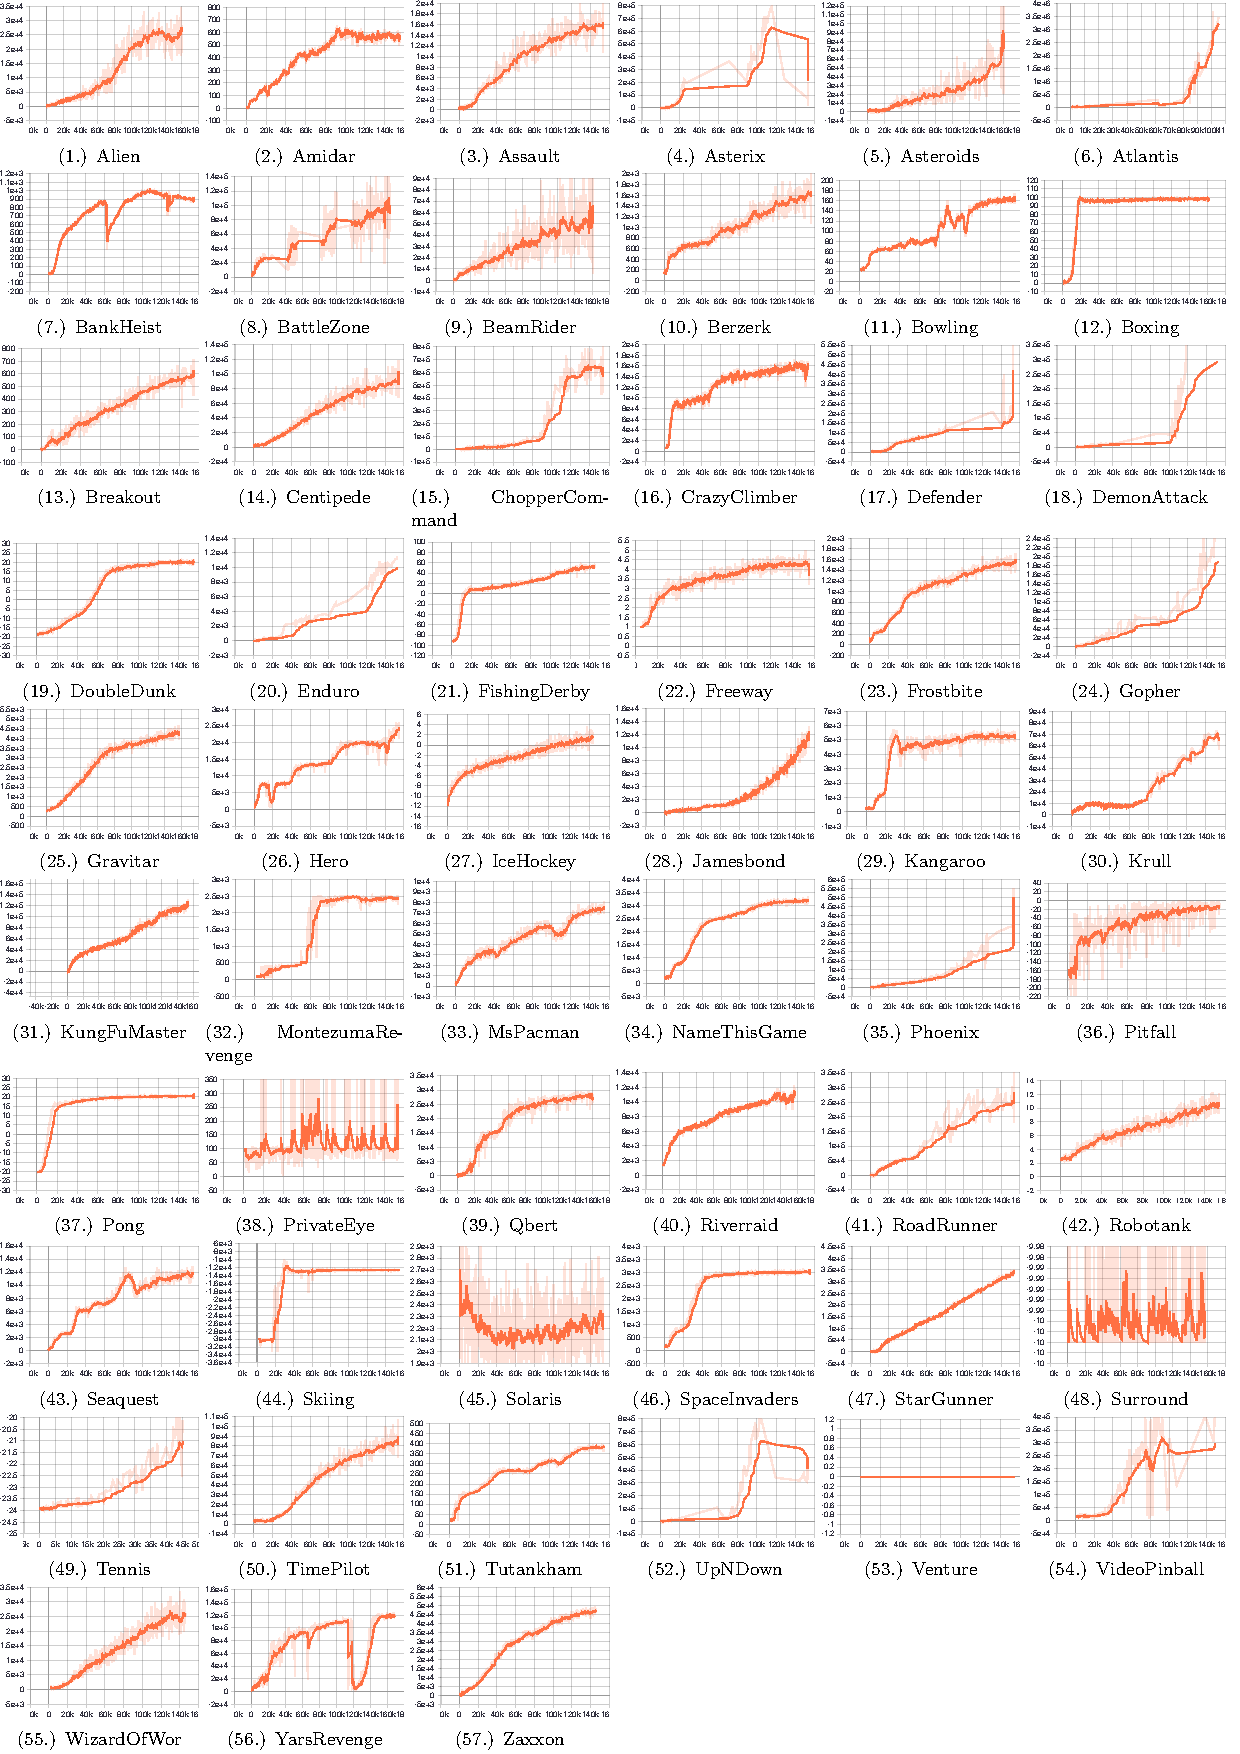
\includegraphics[width=1.0\linewidth]{body/all_fig3.pdf}
\end{figure*}

\clearpage



\end{document}
